% #############################################################################
% This is the MAIN DOCUMENT of the Thesis MSc TEMPLATE.
% The content for the Thesis MSc is to be written in separate documents
% located in the folder ./Chapters
%         Aknowledgments.tex
%         Abstract.tex
%         KeyWords.tex
%         Resumo.tex
%         PalavrasChave.tex
%         Acronyms.tex
%         Front_Cover.tex
%         Chapter_1.tex ....Chapter_2 .....
%         ApendixA.tex ... ApendixB.tex...
% -----------------------------------------------------------------------------
% The class "istulthesis" is based on the standard LaTeX 'report' class.
% It can be used for Instituto Superior Tecnico thesis, as it follows the 
% regulations published by the Scientific Council of IST.
% The class defines the document style. 
% IST requires the thesis to be written in Arial or similar. 
% Two arguments in '\documentclass' allow you to define the thesis font: 
% 'Helvetica' and 'AvantGarde', which transforms 
% the default LaTeX font into Helvetica or AvantGarde, respectively.
% #############################################################################
% The document is automatically set for english or portuguese by just selecting
% the MAIN LANGUAGE in file 'Thesis-MSc-Preamble_commands.tex' 
% #############################################################################
% Thesis-MSc
% Version 2.0, August 2018
% BY: Rui Santos Cruz, rui.s.cruz@tecnico.ulisboa.pt
% #############################################################################
% !TEX root = ./main.tex
% -----------------------------------------------------------------------------
%
\documentclass[defaultstyle,10pt,Helvetica]{istulthesis}
%
% -----------------------------------------------------------------------------
% The Preamble document contains all the necessary Packages for typesetting
% Modify it to suit your needs
% -----------------------------------------------------------------------------
% #############################################################################
% Preamble for Thesis-MSc in English or Portuguese
% Required Packages and commands
% --> Please Choose the MAIN LANGUAGE for the Thesis in package BABEL (below)
% !TEX root = ./main.tex
% #############################################################################
% Thesis-MSc
% Version 2.0, August 2018
% BY: Rui Santos Cruz, rui.s.cruz@tecnico.ulisboa.pt
% #############################################################################
%
% -----------------------------------------------------------------------------
% PACKAGES ucs, utf8x, babel, iflang:
% -----------------------------------------------------------------------------
% The 'ucs' package provides support for using UTF-8 in LaTeX documents. 
% However in most situations it is not required.
\usepackage{ucs}
% The 'utf8x' package contains support for using UTF-8 as input encoding. 
\usepackage[utf8x]{inputenc}
% The 'babel' package may correct some hyphenation issues of LaTeX. 
% Select your MAIN LANGUAGE for the Thesis with the 'main=' option.
\usepackage[main=english,portuguese]{babel}
% The 'iflang' package is used to help determine the language being used. 
\usepackage{iflang}

% -----------------------------------------------------------------------------
% PACKAGE scrbase:
% -----------------------------------------------------------------------------
% The 'scrbase' package is used to help redefining document structure.
\usepackage{scrbase}
% -----------------------------------------------------------------------------
% PACKAGE mathtools, amsmath, amsthm, amssymb, amsfonts, nicefrac:
% -----------------------------------------------------------------------------
% These packages are typically required. 
% Among many other things they add the possibility to put symbols in bold
% by using \boldsymbol (not \mathbf); defines additional fonts and symbols;
% adds the \eqref command for citing equations.
\usepackage{mathtools, amsmath, amsthm, amssymb, amsfonts}
\usepackage{nicefrac}
%
% -----------------------------------------------------------------------------
% PACKAGE tikz:
% -----------------------------------------------------------------------------
% Tikz  for creating graphics programmatically.
\usepackage{tikz}
\usetikzlibrary{shapes.geometric, arrows, positioning}
% -----------------------------------------------------------------------------
% PACKAGES array, booktabs, multirow, colortbl, ctable, spreadtab:
% -----------------------------------------------------------------------------
% These packages are most usefull for advanced tables. 
% 'multirow' allows to join rows throuhg the command \multirow which works
% similarly with the command \multicolumn.
% The 'colortbl' package allows to color the table (foreground and background)
% The 'ctable' package provides commands to easily typeset centered or left or
% right aligned tables.
% The package 'booktabs' provide some additional commands to enhance
% the quality of tables
% The 'longtable' package is only required when tables extend beyond the length
% of one page, which typically does not happen and should be avoided
\usepackage{array}
\usepackage{booktabs}
\usepackage{multirow}
\usepackage{colortbl}
\usepackage{ctable}
\usepackage{spreadtab}
\usepackage{longtable}
%
% -----------------------------------------------------------------------------
% PACKAGES graphicx, subfigure:
% -----------------------------------------------------------------------------
% The package 'graphicx' supports formats PNG and JPG.
% Package 'subfigure' allows to place figures within figures with own caption. 
% For each of the subfigures use the command \subfigure.
\usepackage{graphicx}
\usepackage[hang,small,bf,tight]{subfigure}
%
% -----------------------------------------------------------------------------
% PACKAGE caption:
% -----------------------------------------------------------------------------
% The 'caption' package offers customization of captions in floating 
% environments such figure and table
% \usepackage[hang,small,bf]{caption}
\usepackage[format=hang,labelfont=bf,font=small]{caption} 
% the following customization adds vertical space between caption and the table
\captionsetup[table]{skip=10pt}
%
% -----------------------------------------------------------------------------
% PACKAGE algorithmic, algorithm, algorithm2e:
% -----------------------------------------------------------------------------
% These packages are required if you need to describe an algorithm.
% The preference is for using 'algorithm2e'
%\usepackage{algorithmic}
%\usepackage[chapter]{algorithm}
\usepackage[ruled,vlined,algochapter,norelsize,\languagename]{algorithm2e}
%
% -----------------------------------------------------------------------------
% PACKAGE listings
% -----------------------------------------------------------------------------
% These packages are required if you need to list code snippets.
\usepackage{listings}
% Nicely syntax highlighted m-code in LaTeX documents with stylefile mcode.sty
% http://www.mathworks.com/matlabcentral/fileexchange/8015-m-code-latex-package
\usepackage[numbered]{./tables_and_code/mcode}
%
% -----------------------------------------------------------------------------
% Re-define listings captions and titles based on language.
\newcaptionname{portuguese}{\lstlistingname}{Listagem} % Listings CAPTIONS
\newcaptionname{portuguese}{\lstlistlistingname}{Listagens} % LIST of LISTINGS
%
% -----------------------------------------------------------------------------
% PACKAGE csquotes
% -----------------------------------------------------------------------------
% Quotation helper package
\usepackage{csquotes}
%
% -----------------------------------------------------------------------------
% PACKAGE todonotes
% -----------------------------------------------------------------------------
% Create TODO Notes in text
% The notes can be made invisible by just using the 'disable' option:
\usepackage[textwidth=2cm, textsize=small]{todonotes}
%\usepackage[textwidth=2cm, textsize=small, disable]{todonotes}
\setlength{\marginparwidth}{2cm}
%
% -----------------------------------------------------------------------------
% PACKAGE changes
% -----------------------------------------------------------------------------
% Track changes in document (changes in pdf preview).
%% Use "final" option to make all tracking markups invisible.
%\usepackage[authormarkup=superscript,authormarkuptext=id,markup=underlined,ulem={ULforem,normalbf},final]{changes}
\usepackage[authormarkup=superscript,authormarkuptext=id,markup=underlined,ulem={ULforem,normalbf}]{changes}
% commands:
% \added[id=xx]{text}
% \deleted[id=xx]{text}
% \replaced[id=xx]{deleted text}{added text}
% -----------------------------------------------------------------------------
% PACKAGES xcolor, color
% -----------------------------------------------------------------------------
% These packages are required for list code snippets.
\usepackage{xcolor}
\usepackage{color}
% The following special color definitions are used in the IST Thesis
\definecolor{forestgreen}{RGB}{34,139,34}
\definecolor{orangered}{RGB}{239,134,64}
\definecolor{lightred}{rgb}{1,0.4,0.5}
\definecolor{orange}{rgb}{1,0.45,0.13}	
\definecolor{darkblue}{rgb}{0.0,0.0,0.6}
\definecolor{lightblue}{rgb}{0.1,0.57,0.7}
\definecolor{gray}{rgb}{0.4,0.4,0.4}
\definecolor{lightgray}{rgb}{0.95, 0.95, 0.95}
\definecolor{darkgray}{rgb}{0.4, 0.4, 0.4}
\definecolor{editorGray}{rgb}{0.95, 0.95, 0.95}
\definecolor{editorOcher}{rgb}{1, 0.5, 0} % #FF7F00 -> rgb(239, 169, 0)
\definecolor{chaptergrey}{rgb}{0.6,0.6,0.6}
\definecolor{editorGreen}{rgb}{0, 0.5, 0} % #007C00 -> rgb(0, 124, 0)
\definecolor{olive}{rgb}{0.17,0.59,0.20}
\definecolor{brown}{rgb}{0.69,0.31,0.31}
\definecolor{purple}{rgb}{0.38,0.18,0.81}
%
% -----------------------------------------------------------------------------
% PACKAGE setspace:
% ----------------------------------------------------------------------------
% Provides support for setting the spacing between lines in a document. 
% Package options include single spacing, one half spacing, and double spacing. 
% Alternatively the spacing can be changed as required with:
% \singlespacing, \onehalfspacing, and \doublespacing commands
\usepackage{setspace}
%
% -----------------------------------------------------------------------------
% PACKAGE paralist
% -----------------------------------------------------------------------------
% This package provides the 'inparaenum' environment for inline lists
\usepackage{paralist}
% usage:
% \begin{inparaenum}[(a)]
% \item bla
% \item bla, bla
% \end{inparaenum}
% -----------------------------------------------------------------------------
% PACKAGE cite:
% -----------------------------------------------------------------------------
% The 'cite' package will result in citation numbers being automatically
% sorted and properly "ranged". i.e.,
% [1], [2], [5]--[7], [9]
\usepackage{cite}
%
% -----------------------------------------------------------------------------
% PACKAGE acronym:
% -----------------------------------------------------------------------------
% The package 'acronym' garantees that all acronyms definitions are 
% given at the first usage. 
% IMPORTANT: do not use acronyms in titles/captions; otherwise the definition 
% will appear on the table of contents.
\usepackage[printonlyused]{acronym}
%
% -----------------------------------------------------------------------------
% PACKAGE hyperref
% -----------------------------------------------------------------------------
% Set links for references and citations in document
\usepackage{hyperref}
% pre-configuration of hyperref
\hypersetup{ colorlinks=true,
             citecolor=cyan,
             linkcolor=darkgray,
             urlcolor=teal,
             breaklinks=true,
             bookmarksnumbered=true,
             bookmarksopen=true,
             pdftitle=\@title, % THESIS TITLE
             pdfauthor=\@author,  % YOUR NAME
             pdfcreator=\@author,   % YOUR NAME
}
%
% -----------------------------------------------------------------------------
% PACKAGE url:
% -----------------------------------------------------------------------------
% Provides better support for handling and breaking URLs.
\usepackage{url} 
%
% -----------------------------------------------------------------------------
% PACKAGE Cleveref:
% -----------------------------------------------------------------------------
% Clever Referencing of document parts
% Note: portuguese is supported through "brazilian" option
\usepackage[\IfLanguageName{english}{english}{brazilian}]{cleveref}
%
% -----------------------------------------------------------------------------
% PACKAGE enumitem:
% -----------------------------------------------------------------------------
%For enhanced enumeration of lists
%\usepackage{enumitem}
\usepackage[shortlabels]{enumitem}
\setlist[description]{leftmargin=\parindent,labelindent=\parindent,itemsep=1pt,parsep=0pt,topsep=0pt}
%
% #############################################################################
% GLOBAL FORMATTING OF THE THESIS DOCUMENT before using FANCY stuff
% Set paragraph counter to alphanumeric mode
\renewcommand{\theparagraph}{\Alph{paragraph}~--}
\hoffset 0in
\voffset 0in
\oddsidemargin 0 cm
\evensidemargin 0 cm
\marginparsep 0in
\topmargin -0.25cm
\textwidth 16 cm
%\textwidth 17 cm
\textheight 22.4 cm
\makeatletter
% package indentfirst says \let\@afterindentfalse\@afterindenttrue
% and we revert this modification, reinstating the original definitio
% of \@afterindentfalse
\def\@afterindentfalse{\let\if@afterindent\iffalse}
\makeatother
% -----------------------------------------------------------------------------
% PACKAGE fancyhdr:
% -----------------------------------------------------------------------------
% The fancyhdr macro package allows to customize page headers and footers.
\usepackage{fancyhdr}
\pagestyle{fancy}
\renewcommand{\chaptermark}[1]{\markboth{\thechapter.\ #1}{}}
\renewcommand{\sectionmark}[1]{\markright{\thesection\ #1}}
\fancyhead{}
\renewcommand{\headrulewidth}{0.0pt}
\renewcommand{\footrulewidth}{0.0pt}
\addtolength{\headheight}{2pt} % make space for the rule
\fancypagestyle{plain}{%
   \fancyhead{} % get rid of headers
   \renewcommand{\headrulewidth}{0pt} % and the line
   \renewcommand{\footrulewidth}{0pt}
}
\fancypagestyle{blank}{%
   \fancyhf{} % get rid of headers and footers
   \renewcommand{\headrulewidth}{0pt} % and the line
   \renewcommand{\footrulewidth}{0pt}
}
\fancypagestyle{abstract}{%
   \fancyhead{}
   \renewcommand{\headrulewidth}{0pt}
   \renewcommand{\footrulewidth}{0.0pt}
}
\fancypagestyle{document}{%
	\fancyhead{}
	\renewcommand{\headrulewidth}{0.5pt}
	\renewcommand{\footrulewidth}{0.5pt}
	\addtolength{\headheight}{2pt} % make space for the rule
}
\setcounter{secnumdepth} {5}
\setcounter{tocdepth} {5}
\renewcommand{\thesubsubsection}{\thesubsection.\Alph{subsubsection}}
\renewcommand{\subfigtopskip}{0.3 cm}
\renewcommand{\subfigbottomskip}{0.2 cm}
\renewcommand{\subfigcapskip}{0.3 cm}
\renewcommand{\subfigcapmargin}{0.2 cm}
%
% -----------------------------------------------------------------------------
% PACKAGE minitoc:
% -----------------------------------------------------------------------------
% Package 'minitoc' creates a mini-table of contents (a “minitoc”) at 
% the beginning of each chapter of a document.
% This packages are required for the \fancychapter configuration
\usepackage{minitoc}
\setcounter{minitocdepth}{1}
\setlength{\mtcindent}{24pt}
\renewcommand{\mtcfont}{\small\rm}
\renewcommand{\mtcSfont}{\small\bf}
\renewcommand*{\kernafterminitoc}{\kern0.\baselineskip\kern0.ex}
\mtcselectlanguage{\languagename} 
% Now prepare the MINITOC
\def\boxedverbatim{%
  \def\verbatim@processline{%
    {\setbox0=\hbox{\the\verbatim@line}%
    \hsize=\wd0 \the\verbatim@line\par}}%
  \@minipagetrue%%%DPC%%%
  \@tempswatrue%%%DPC%%%
  \setbox0=\vbox\bgroup\vspace*{0.2cm}\footnotesize\verbatim
}
\def\endboxedverbatim{%
  \endverbatim
  \unskip\setbox0=\lastbox %%%DPC%%%
  \hspace*{0.2cm}
  \vspace*{-0.2cm}
  \egroup
  \fbox{\box0}% <<<=== change here for centering,...
}
% Now prepare the CHAPTER Number
\newcommand*{\chapnumfont}{%
%   \usefont{T1}{\@defaultcnfont}{b}{n}\fontsize{100}{130}\selectfont%
  \usefont{T1}{pbk}{b}{n}
  \fontsize{150}{130}
  \selectfont
  \color{chaptergrey}
}
\makeatletter
\def\@makechapterhead#1{%
  \vspace*{50\p@}%
  {\parindent \z@ \raggedright \normalfont
    {\chapnumfont\ifnum \c@secnumdepth >\m@ne
%         \huge\bfseries \@chapapp\space \thechapter
        \raggedleft\bfseries \thechapter
        \par\nobreak
        \vskip 20\p@
    \fi}
    \interlinepenalty\@M
    {\raggedleft\Huge \bfseries #1\par\nobreak}
    \vskip 40\p@
  }}
\makeatother
% Now put it all together as a command \fancychapter
\newcommand{\fancychapter}[1]{\chapter{#1}\vfill\minitoc\pagebreak}
%
% #############################################################################
% ADDITIONAL COMMANDS AND CONFIGURATIONS
% #############################################################################
% This commmand allows to place horizontal lines with a custom width... 
% replaces the standard hline command
\newcommand{\hlinew}[1]{%
  \noalign{\ifnum0=`}\fi\hrule \@height #1 \futurelet
   \reserved@a\@xhline}
%   
% -----------------------------------------------------------------------------
% This command defines some marks... USEFUL FOR TABLES.
\def\Mark#1{\raisebox{0pt}[0pt][0pt]{\textsuperscript{\footnotesize\ensuremath{\ifcase#1\or *\or \dagger\or \ddagger\or%
    \mathsection\or \mathparagraph\or \|\or **\or \dagger\dagger%
    \or \ddagger\ddagger \else\textsuperscript{\expandafter\romannumeral#1}\fi}}}}
%
% -----------------------------------------------------------------------------
% The following configurations are used for LISTINGS of certain languages
\lstdefinestyle{XML} {
	language=XML,
	extendedchars=true, 
	breaklines=true,
	breakatwhitespace=true,
	emph={},
	emphstyle=\color{red},
	basicstyle=\small,
	xleftmargin=17pt,
	columns=fullflexible,
	commentstyle=\color{gray}\upshape,
	morestring=[b][\color{brown}]",
	morecomment=[s]{<?}{?>},
	morecomment=[s][\color{forestgreen}]{<!--}{-->},
	keywordstyle=\color{orangered},
	stringstyle=\ttfamily\color{black},
	% stringstyle=\ttfamily\color{black}\normalfont,
	tagstyle=\color{blue},
	% tagstyle=\color{darkblue}\bf,
	morekeywords={asn,action,addrType,abilityNAT,audioSampleRate,audiChannels,,bandwidth,bitmapSize,bitRate,connection,codecs,concurrentLinks,dependency,duration,frameRate,from,height,ip,id,lang,mimeType,onlineTime,peerMode,port,priority,peerProtocol,property,release,to,tier,type,transactionID,url,uploadBWlevel,version,width},
	otherkeywords={attribute,xmlns,schemaLocation,PresentationType,availabilityStartTime,availabilityEndTime,minimumUpdatePeriod,minBufferTime,UpdateTime},
}
% ----------------------------------------------------------------------------
\lstdefinelanguage{Assembler}{
	morecomment=[l];,
	keywords={ADD,ADDC,SUB,SUBB,CMP,MUL,DIV,MOD,NEG,AND,OR,NOT,XOR,TEST,BIT,SET,EI,EI0,EI1,EI2,EI3,SETC,EDMA,CLR,DI,DI0,DI1,DI2,DI3,CLRC,SHR,SHL,SHRA,SHLA,ROR,ROL,RORC,ROLC,MOV,MOVB,MOVBS,MOVP,MOVL,MOVH,SWAP,PUSH,POP,JZ,JNZ,JN,JNN,JP,JNP,JC,JNC,JV,JNV,JEQ,JNE,JLT,JLE,JGT,JGE,JA,JAE,JB,JBE,JMP,CALL,CALLF,RET,RETF,SWE,RFE,NOP},
	morekeywords={EQU,TABLE,WORD,STRING,PLACE},
} 
% ----------------------------------------------------------------------------
\lstdefinestyle{coloredASM}{
	language=Assembler,
	extendedchars=false,
	breaklines=true,
	tabsize=2,
	numberstyle=\tiny,
	numbers=left,
	breakatwhitespace=true,
	emph={},
	emphstyle=\color{red},
	fontadjust=true,
	basicstyle=\small\ttfamily,
	% basicstyle=\footnotesize\ttfamily,
	columns=fixed,
	xleftmargin=17pt,
	framexleftmargin=17pt,
	framexrightmargin=5pt,
	framexbottommargin=4pt,
	commentstyle=\color{forestgreen}\upshape,
	morestring=[b][\color{brown}]",
	keywordstyle=\color{darkblue},
	stringstyle=\ttfamily\color{black},
	literate={á}{{\'a}}1 {ã}{{\~a}}1 {â}{{\^a}}1 {é}{{\'e}}1 {É}{{\'E}}1 {ê}{{\^e}}1 {õ}{{\~o}}1 {ó}{{\'o}}1 {í}{{\'i}}1 {ç}{{\c{c}}}1 {Ç}{{\c{C}}}1,
}    
% ----------------------------------------------------------------------------
\lstdefinelanguage{CSS}{
	sensitive=true,
	morecomment=[l]{//},
	morecomment=[s]{/*}{*/},
	morestring=[b]',
	morestring=[b]",
	alsoletter={:},
	alsodigit={-},
	keywords={color,background-image:,margin,padding,font,weight,display,position,top,left,right,bottom,list,style,border,size,white,space,min,width, transition:, transform:, transition-property, transition-duration, transition-timing-function}
}
% ----------------------------------------------------------------------------
% JavaScript
\lstdefinelanguage{JavaScript}{
	morecomment=[s]{/*}{*/},
	morecomment=[l]//,
	morestring=[b]",
	morestring=[b]',
	morekeywords={typeof, new, true, false, catch, function, return, null, catch, switch, var, if, in, while, do, else, case, break}
}
% ----------------------------------------------------------------------------
\lstdefinelanguage{HTML5}{
	language=html,
	sensitive=true,	
	alsoletter={<>=-},	
	morecomment=[s]{<!-}{-->},
	tag=[s],
	otherkeywords={
	% General
	>,
	% Standard tags
	<!DOCTYPE,
	</html, <html, <head, <title, </title, <style, </style, <link, </head, <meta, />,
	% body
	</body, <body,
	% Divs
	</div, <div, </div>, 
	% Paragraphs
	</p, <p, </p>,
	% scripts
	</script, <script,
	% More tags...
	<canvas, /canvas>, <svg, <rect, <animateTransform, </rect>, </svg>, <video, <source, <iframe, </iframe>, </video>, <image, </image>, <header, </header, <article, </article},
	ndkeywords={
	% General
	=,
	% HTML attributes
	charset=, src=, id=, width=, height=, style=, type=, rel=, href=,
	% SVG attributes
	fill=, attributeName=, begin=, dur=, from=, to=, poster=, controls=, x=, y=, repeatCount=, xlink:href=,
	% properties
	margin:, padding:, background-image:, border:, top:, left:, position:, width:, height:, margin-top:, margin-bottom:, font-size:, line-height:,
	% CSS3 properties
	transform:, -moz-transform:, -webkit-transform:,
	animation:, -webkit-animation:,
	transition:,  transition-duration:, transition-property:, transition-timing-function:,
	}
}
% ----------------------------------------------------------------------------
\lstdefinestyle{htmlcssjs} {%
	% General design
	backgroundcolor=\color{editorGray},
		fontadjust=true,
	basicstyle=\small\ttfamily,   
	frame=b,
	% line-numbers
	xleftmargin={0.75cm},
	numbers=left,
	stepnumber=1,
	firstnumber=1,
	numberfirstline=true,	
	% Code design
	identifierstyle=\color{black},
	keywordstyle=\color{blue}\bfseries,
	ndkeywordstyle=\color{editorGreen}\bfseries,
	stringstyle=\color{editorOcher}\ttfamily,
	commentstyle=\color{brown}\ttfamily,
	% Code
	language=HTML5,
	alsolanguage=JavaScript,
	alsodigit={.:;},	
	tabsize=2,
	showtabs=false,
	showspaces=false,
	showstringspaces=false,
	extendedchars=true,
	breaklines=true,
	% German umlauts
	literate=%
	{Ö}{{\"O}}1
	{Ä}{{\"A}}1
	{Ü}{{\"U}}1
	{ß}{{\ss}}1
	{ü}{{\"u}}1
	{ä}{{\"a}}1
	{ö}{{\"o}}1
}
% ----------------------------------------------------------------------------
\lstdefinestyle{py} {%
	language=python,
	literate=%
	*{0}{{{\color{lightred}0}}}1
	{1}{{{\color{lightred}1}}}1
	{2}{{{\color{lightred}2}}}1
	{3}{{{\color{lightred}3}}}1
	{4}{{{\color{lightred}4}}}1
	{5}{{{\color{lightred}5}}}1
	{6}{{{\color{lightred}6}}}1
	{7}{{{\color{lightred}7}}}1
	{8}{{{\color{lightred}8}}}1
	{9}{{{\color{lightred}9}}}1,
	basicstyle=\small\ttfamily,
	numbers=left,
	% numberstyle=\tiny,
	% stepnumber=2,
	numbersep=5pt,
	tabsize=4,
	extendedchars=true,
	breaklines=true,
	keywordstyle=\color{blue}\bfseries,
	frame=b,
	commentstyle=\color{brown}\itshape,
	stringstyle=\color{editorOcher}\ttfamily,
	showspaces=false,
	showtabs=false,
	xleftmargin=17pt,
	framexleftmargin=17pt,
	framexrightmargin=5pt,
	framexbottommargin=4pt,
	backgroundcolor=\color{lightgray},
	showstringspaces=false,
}
%
% #############################################################################
% #############################################################################
\begin{document}
%
% Add PDF bookmark 
\pdfbookmark[0]{Multi-Objective Optimization}{Multi-Objective Optimization in Architecture}
% #############################################################################
% DEFINE THE Front Cover Page of Thesis-MSc
% !TEX root = ./main.tex
% #############################################################################
% Thesis-MSc
% Version 2.0, August 2018
% BY: Rui Santos Cruz, rui.s.cruz@tecnico.ulisboa.pt
% #############################################################################
%
% REQUIRED LOGO:
% The university logo image: arguments correspond to {left}{top} position. 
% IST rules determine the position to be be 2cm from top, left page edge
\univlogo{2cm}{2cm}{./Images/IST_A_RGB_POS}
% OPTIONAL IMAGE:
% The thesis image: arguments are the start position in the page.
% You can change the image for your thesis, replacing the image name:
%\thesislogo{2.5cm}{6cm}{./Images/thesis_logo}
%\thesislogo{2.5cm}{6cm}{./Images/tecnico-lisboa}
%
% -----------------------------------------------------------------------------
% REQUIRED: Thesis TITLE
\title{Optimization of Complex Design Problems in Architecture}
% OPTIONAL: Thesis SUBTITLE
%\subtitle{This is the Thesis Subtitle if Necessary}
%
% -----------------------------------------------------------------------------
% REQUIRED: Author
% Author full Name
\author{Catarina Garcia Belém}
%
% -----------------------------------------------------------------------------
% The official name of the course/degree. Please chose portuguese or english
% un-comment the line corresponding to your degree.
% You can add a degree name using this construct
%
\degree{Information Systems and Computer Engineering}
%\degree{Engenharia Informática e de Computadores}
%\degree{Telecommunications and Informatics Engineering}
%\degree{Engenharia de Telecomunicações e Informática}
%
% -----------------------------------------------------------------------------
% REQUIRED: The SUPERVISOR(s) - maximum of two
\supervisor{Prof. António Paulo Teles de Menezes Correia Leitão}
% If no co-Supervisor comment the next line
% \othersupervisor{Prof. Name of the Co-Supervisor}
%
% -----------------------------------------------------------------------------
% REQUIRED: Date of examination
% Insert the Date of the Thesis discussion (format is MONTH and YEAR)
\date{May 2019}
%
% -----------------------------------------------------------------------------
% The following command define the author colors for Tracking Changes in doc
\definechangesauthor[color=forestgreen]{MN}
\definechangesauthor[color=blue]{JO}
\definechangesauthor[color=red]{PT}

% -----------------------------------------------------------------------------
% Place 'false' when delivering the draft version of the thesis.
% The committee members should not be printed for the draft version. 
% Place 'true' after the Examination Committee has accepted the thesis as final
%\finalthesis{true}
\finalthesis{false}
%
% -----------------------------------------------------------------------------
% The members of the Examination Committee
\chairperson{Prof. Ernesto José Marques Morgado}
\vogalone{Prof. Name of First Committee Member}
%\vogaltwo{Dr. Name of Second Committee Member}
%\vogalthree{Eng. Name of Third Committee Member}
%
% -----------------------------------------------------------------------------
% Please DO NOT MODIFY the following lines.
% print the titlepage
\maketitle
\clearpage
\thispagestyle{empty}
% If Printing on DOUBLE SIDED pages, the second page should be white.
\cleardoublepage
%
% -----------------------------------------------------------------------------
% PAGE NUMBERING FOR INDEXING MATTER in ROMAN
\setcounter{page}{1} \pagenumbering{roman}
\baselineskip 18pt % line spacing: -12pt for single spacing
                   %               -18pt for 1 1/2 spacing
                   %               -24pt for double spacing
% -----------------------------------------------------------------------------
% THE ACKNOWLEGMENTS
\pdfbookmark[0]{Acknowledgments}{acknowledgments}
\begin{acknowledgments}
	% #############################################################################
% Agradecimentos / Acknowledgments
% !TEX root = ../main.tex
% #############################################################################

I would like to express my respect and gratitude to my supervisor and friend Dr. António Menezes Leitão. He proposed an interesting theme, which proved to be intriguing and challenging. His efforts to arrange research grants and to supply better computational resources were inspiring and encouraged me to fight the difficulties found along the way. His constant support, preoccupation and first-class guidance were invaluable through this thesis. Thanks for everything, especially for encouraging me to pursuit my dreams and for providing me with the flexibility and free-will to tackle this theme as something that I would be proud of.  

I would like to thank the members of the research group oriented by my supervisor, Algorithmic Design for Architecture, for their support and valuable ideas and discussions which undoubtedly improved the practicality of this work - especially, Inês Caetano, Inês Pereira, Renata Castelo Branco, Guilherme Ilunga, and Luís Silveira Santos. 

I would also like to thank the Department of Computer Science and Engineering at Instituto Superior Técnico, Universidade de Lisboa for providing me with the foundations for completing this work, as well as for the opportunities to lecture as a teaching assistant during my MSc Thesis. 

I would also like to thank Instituto de Engenharia de Sistemas e Computadores - Investigação e Desenvolvimento (INESC-ID) for the financial support provided to me in the form of Research Grants.

%I am also grateful to the staff and teachers of the Computer Engineering and Information Systems course for their effort, dedication, availability, and for providing an interesting working environment. 

To all my friends whose support was invaluable during this period and which encouraged me to constantly push my limits when the task felt too large, I thank you deeply from my heart - especially, Carolina Pereira, Cristiana Tiago, Diogo Magalhães, Filipe Magalhães, Gonçalo Rodrigues, Guilherme Ilunga, Nuno Afonso, Pedro Simão, and Telma Correia.

Last but not least, I would like to thank my parents for their friendship, encouragement and caring over all these years, for always being there for me through thick and thin and without whom this project would not be possible. I would also like to thank my sister, brother, and sister-in-law, for their understanding, support, and preoccupation throughout this year.

To each and every one of you -- Thank you.
\end{acknowledgments}
%
% -----------------------------------------------------------------------------
% THE ABSTRACT
\pdfbookmark[0]{Abstract}{Abstract}
\begin{abstract}
	% #############################################################################
% Abstract Text
% !TEX root = ../main.tex
% #############################################################################
% use \noindent in firts paragraph
\noindent 
%  O resumo analítico, também designado por resumo ou abstract, descreve o objectivo, o conteúdo do trabalho e as conclusões. Deve ser escrito em português e inglês, com um máximo de 250 palavras cada e acompanhado de 4 a 6 palavras-chave;

The building sector currently presents one of the largest economic and environmental footprints. Optimization can minimize this impact by finding more efficient building variants, prior to their construction. Building design optimization spurs the exploration of (1) algorithmic approaches, to generate multiple design variants, (2) simulation tools, to evaluate design's performance regarding distinct aspects (e.g., acoustics, thermal, structural, costs), and (3) optimization algorithms, to seek more efficient design variants. Unfortunately, despite the existence of several optimization algorithms, their application to architectural optimization problems is not well-studied and the lack of experience/knowledge often drives architects towards the application of the simplest available algorithm. However, this rarely is the most efficient option for addressing a specific problem, in particular, due to the time-intensive simulations required to evaluate designs. As a result, a poor algorithm selection might lead to unacceptable optimization times and less efficient designs. 

This dissertation evaluates and proposes optimization algorithms specifically tailored for addressing simulation-based optimization problems. In particular, we develop and assess an optimization framework in the context of three architectural case studies involving single- and multi-objective optimization of simulation-based lighting, structural, and cost aspects of buildings. Obtained results reveal that the algorithm that better addresses a specific optimization problem can yield considerable better solutions and/or produce them in considerable less computation time. Moreover, results corroborate the idea that different optimization algorithms should be tested in order to determine the one that better fits the problem to address. Finally, this dissertation shows the benefits of optimization to reduce the impact of the building sector and motivates its introduction as an indispensable phase of the architectural design process.

\end{abstract}
\begin{keywords}
	% #############################################################################
% English Keywords
% !TEX root = ../main.tex
% #############################################################################
% use \noindent in firts paragraph
\noindent Algorithmic Design; Algorithmic Analysis; Algorithmic Optimization; Derivative-Free Optimization; Surrogate-based Modeling
\end{keywords}
\clearpage
\thispagestyle{empty}
%% If Printing on DOUBLE SIDED pages, the second page should be white.
%% Otherwise, comment the following command:
\cleardoublepage
%
% -----------------------------------------------------------------------------
% O RESUMO
\pdfbookmark[0]{Resumo}{Resumo}
\begin{resumo}
	% #############################################################################
% RESUMO em Português
% !TEX root = ../main.tex
% #############################################################################
% use \noindent in firts paragraph
\noindent 
O sector da construção representa uma das maiores pegadas económicas e ambientais. Optimização baseada no desempenho de edifícios pode minimizar este impacto ao combinar (1) abordagens algorítmicas, para geração de múltiplas variações do design do edifício, (2) ferramentas de simulação, para avaliar desempenho de um design em relação a vários aspectos, e (3) algoritmos de optimização para procurar os designs mais eficientes. Infelizmente, apesar da existência de vários algoritmos de optimização, a sua aplicação a problemas em arquitectura ainda não foi muito explorada, levando os arquitectos a frequentemente optarem por algoritmos facilmente acessíveis e simples. No entanto, esta raramente é a escolha mais eficiente para resolver um problema específico, em particular, porque para avaliar o design de edíficios é necessário recorrer a simulações computacionalmente pesadas. Como consequência, a má escolha de um algoritmo de optimização pode levar a tempos de execução inaceitáveis, assim como a designs menos eficientes.

Esta dissertação foca-se em algoritmos de optimização especialmente desenhados para lidar com problemas de otimização baseados em simulação. Em particular, nós desenvolvemos e avaliamos uma framework de optimização no contexto de três casos de estudo em arquitectura que involvem a optimização único e múltiplo objectivo dos aspetos lumínicos, estruturais, e de custo dos edíficios. Os resultados obtidos revelam que a qualidade das soluções e o tempo dispendido na optimização dependem fortemente da escolha de algoritmo. Deste modo, diferentes algoritmos devem ser testados de modo a determinar aquele que melhor satisfaz um problema de optimização. Finalmente, esta dissertação demonstra os benefícios da optimização para reduzir o impacto do sector de construção e motiva a sua introdução como uma fase indispensável no processo de design arquitectónico.


\end{resumo}
\begin{palavraschave}
	% #############################################################################
% Portuguese Keywords
% !TEX root = ../main.tex
% #############################################################################
% use \noindent in firts paragraph
\noindent Design Algorítmico; Otimização de caixa-preta; Modelos baseados em aproximações; Aprendizagem Máquina.
\end{palavraschave}
\clearpage
\thispagestyle{empty}
%% If Printing on DOUBLE SIDED pages, the second page should be white.
%% Otherwise, comment the following command:
\cleardoublepage
%
% -----------------------------------------------------------------------------
% This is required for the Fancy Chapters with minitoc
\dominitoc
\dominilof
\dominilot
% -----------------------------------------------------------------------------
% Lists of Contents
\renewcommand{\baselinestretch}{1}
\pdfbookmark[0]{Contents}{toc}
\tableofcontents
%\contentsline{chapter}{References}{\pageref{bib}}
% If Printing on DOUBLE SIDED pages, the second page should be white.
% Otherwise, comment the following command:
\cleardoublepage
% reposition baseline
\renewcommand{\baselinestretch}{1.5}
% -----------------------------------------------------------------------------
% List of Figures
\pdfbookmark[1]{List of Figures}{lof}
\listoffigures
\cleardoublepage
% -----------------------------------------------------------------------------
\begingroup 
    \let\clearpage\relax
    \let\cleardoublepage\relax
    \let\cleardoublepage\relax
% List of Tables
\pdfbookmark[1]{List of Tables}{lot}
\listoftables
% If Printing on DOUBLE SIDED pages, the second page should be white.
% Otherwise, comment the following command:
\let\cleardoublepage\relax
%\cleardoublepage
% -----------------------------------------------------------------------------
% List of Algorithms
% If not used, comments the lines!
% Requires packages algorithmic, algorithm
\pdfbookmark[1]{List of Algorithms}{loa}
\listofalgorithms
% If Printing on DOUBLE SIDED pages, the second page should be white.
\endgroup
% Otherwise, comment the following command:
\cleardoublepage
% -----------------------------------------------------------------------------
% Listings
% If not used, comments the lines!
% Requires packages listings
\pdfbookmark[1]{Listings}{lol}
\lstlistoflistings
\cleardoublepage
% -----------------------------------------------------------------------------
% % List of acronyms
\pdfbookmark[1]{Acronyms}{loac}
\chapter*{\tlangAcronyms}
% #############################################################################
% This is the ACRONYMS Definition
% !TEX root = ../main.tex
% #############################################################################

\begin{acronym}[H.264/SVC]
	% A	--------------------------------------------------------------
	\acro{AD}{Algorithmic Design}
	\acro{AA}{Algorithmic Analysis}
	\acro{AO}{Algorithmic Optimization}
	\acro{API}{Application Programming Interface}
	\acro{aPF}{approximated Pareto Front}
	
	% B --------------------------------------------------------------
	\acro{BIM}{Building Information Modeling}
	\acro{BPO}{Building Performance Optimization}
	\acro{BPS}{Building Performance Simulation}
	
	% C --------------------------------------------------------------
	\acro{CAD}{Computer-Aided Design}
	\acro{cPF}{combined Pareto Front}
	
	% D --------------------------------------------------------------
	\acro{DFO}{Derivative-Free Optimization}
	\acro{DMS}{Direct MultiSearch}
	\acro{DIRECT}{DIviding RECTangles}
	
	% E --------------------------------------------------------------
	\acro{EA}{Evolutionary Algorithm}	
	\acro{ER}{Error Ratio}	
	%\acrodefplural{ES}{Evolution Strategies}
	\acro{ES}{Evolution Strategy}		
	
	% G --------------------------------------------------------------
	\acro{GA}{Genetic Algorithm}
	\acro{GD}{Generational Distance}
	\acro{GPR}{Gaussian Process Regressor}
	\acro{GUI}{Graphical User Interface}
	
	% H --------------------------------------------------------------
	\acro{HV}{Hypervolume}

	% I --------------------------------------------------------------
	\acro{IGD}{Inverted Generational Distance}
	
	% L --------------------------------------------------------------

	% M	--------------------------------------------------------------
	\acro{ML}{Machine Learning}
	\acro{MLP}{Multi-Layer Perceptron}
	\acro{MOEA}{Multi-Objective Evolutionary Algorithm}
	\acro{MPFE}{Maximum Pareto Front Error}
	\acro{MOO}{Multi-Objective Optimization}
	\acro{MOOA}{Multi-Objective Optimization Algorithm}
	
	% N --------------------------------------------------------------
	\acro{NFLT}{No Free Lunch Theorem}	
	\acro{NN}{Neural Network}	
	\acro{NMS}{Nelder-Mead Simplex}
	\acro{NSGA-II}{Non-dominated Sorting Genetic Algorithm II}
	
	% O --------------------------------------------------------------	
	\acro{ONVG}{Overall Non-dominated Vector Generation}
	\acro{ONVGR}{Overall Non-dominated Vector Generation Ratio}
	
	
	% P --------------------------------------------------------------
	\acro{PBD}{Performance-Based Design}
	\acro{PRAXIS}{Principal Axis}
	\acro{PSO}{Particle-Swarm Optimization}
	
	% R	--------------------------------------------------------------
	\acro{RBF}{Radial Basis Function}	
	\acro{RF}{Random Forest}	
			
	% S	--------------------------------------------------------------
	\acro{sUDI}{spatial Useful Daylight Illumination}
	\acro{SPEA2}{Strength Pareto Evolutionary Algorithm 2}
	\acro{SOO}{Single-Objective Optimization}
	\acro{SVM}{Support Vector Machine}
	% T	--------------------------------------------------------------
	\acro{tPF}{true Pareto Front}
	
\end{acronym}
% If Printing on DOUBLE SIDED pages, the second page should be white.
% Otherwise, comment the following command:
\cleardoublepage
% -----------------------------------------------------------------------------
% PAGE NUMBERING FOR DOCUMENT MATTER in ARABIC
% Pages number is starting with arabic style. Until here were on roman mode
\setcounter{page}{1} \pagenumbering{arabic}
\baselineskip 18pt
% -----------------------------------------------------------------------------
% This a suggestion for the Content of the Document
% Add more Chapters by duplicating a Chapter Block, pointing to the file
%Chapter 1
\acresetall
% #############################################################################
% This is Chapter 1
% !TEX root = ../main.tex
% #############################################################################
% Change the Name of the Chapter i the following line
\fancychapter{Introduction}
\cleardoublepage
% The following line allows to ref this chapter
\label{chap:intro}
	
	The act of making things as perfect, functional, or effective as possible is a process known as optimization~\cite{MerriamWebster2017OptimizationDefinition}. Intuitively, through optimization one aims to improve different quantitative measurable aspects. However, sometimes, instead of trying to achieve perfection, finding a better outcome or a near-optimal one suffices. %Although usually striving to fully optimize, i.e., to obtain \textit{perfection}, in some cases, finding a better outcome or a near-optimal one suffices.
	
	Optimization has a paramount impact in the fields of economy, science, and engineering, among others. As a case in point, optimization yields great potential to the architecture field, as it directly impacts the building industry: optimization enables the reduction of the economic and ecological footprint of the building sector through the finding of more efficient building variants, prior to their construction. 
	
	Modern architecture has grown to incorporate economic and environmental concerns into its building design practices by introducing standardized building regulations and energy certificates. These concerns led to the creation of new design approaches, such as \ac{PBD} which seeks for more efficient design solutions by considering the design's performance, possibly measured by using computational tools~\cite{Oxman2006PBD}.
	
	One example of the \ac{PBD} approach is the City Hall in London, shown in \cref{fig:cityhalllondon}. The building was designed to achieve optimum energy performance by minimizing the surface area exposed to direct sunlight, thus originating its spherical-like form. The application of energy-saving techniques, such as leaning the building outwards so that the floorplates provide shading to the floors below, or the use of groundwater from the water table to supply the building's cooling system, reduced the need for additional cooling devices and, consequently, enabled the energy consumed by the building to be 75\% lower than the energy consumed by typical air-conditioned office buildings \cite{Malkawi2005}.
	% , the use of groundwater from the water table to supply the building's cooling system, and the use of photovoltaic panels on the top of the building to maximize direct sunlight,
	\begin{figure}[htbp]
		\centering
		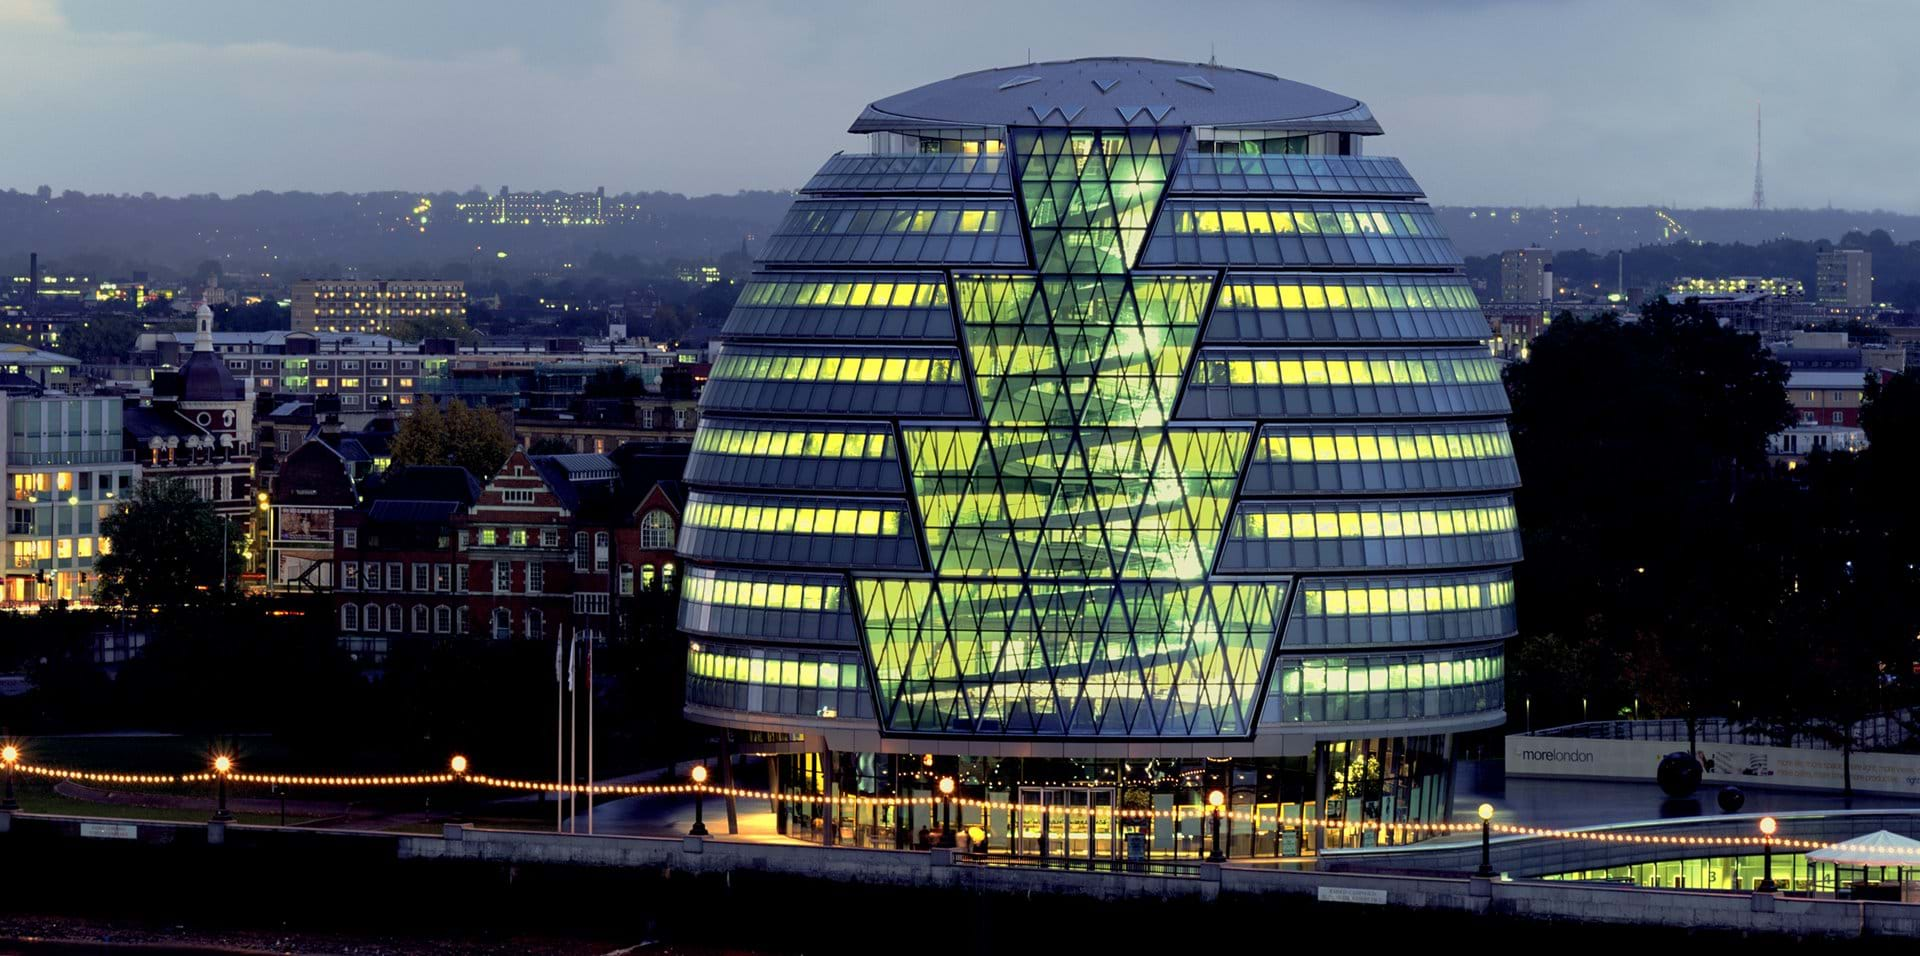
\includegraphics[width=\textwidth]{./Images/Introduction/cityhalllondon.jpg}
		\caption[City Hall in London, designed by Foster and Partners]{City Hall in London, designed by Foster+Partners. Image retrieved from \cite{londoncityhall}.}
		\label{fig:cityhalllondon}
	\end{figure}

	Notwithstanding the benefits attained with \ac{PBD}, to achieve the most performant designs regarding a certain aspect (e.g., lighting, structural, cost),the evaluation of multiple design variants is required. However, even a single evaluation may take up to several seconds, minutes, hours, or days to complete. This is particularly problematic in building design, which frequently requires the evaluation of multiple conflicting aspects, e.g., maximum lighting and thermal comfort, and minimum energy consumption. Adding to this complexity, \ac{PBD} approaches often require architects to perform several manual and time-consuming interventions in order to guarantee that the results meet the standard requirements. The constant need for manual interventions and the time complexity limit the number of design variations evaluated during a \ac{PBD} approach and, consequently, lead to designs that are far from being optimal.  
	
	Given the relevance of \ac{PBD} to the world's sustainability and economy, this dissertation attempts to automate the \ac{PBD} process and, consequently, maximize its potential to the architectural practice. To this end, we address optimization algorithms especially targeted to solve problems involving expensive evaluation functions and to develop an optimization framework that supports their application within the architectural practice to create optimized designs. To better understand which algorithms to use and how to tackle \ac{PBD}'s time limitations, we must consider its two main stages: design and analysis. While in the former, the architect creates a design, in the latter, the architect evaluates the design's performance, possibly by using computational analysis tools. To deal with the exploration of several design alternatives, this dissertation proposes a framework capable of generating and evaluating design variants, using the results of each evaluation to search for more efficient designs.
	
	The following sections of this chapter describe the evolution of the optimization practice in architecture, evidencing the limitations of different design processes and the foundations for the creation of an automatic optimization framework for architecture. Finally, we end by highlighting the dissertation's research goals and its structure.

%% #############################################################################
\section{From Design to Optimized Design}
	
	In architecture, optimization has been gaining relevance for the past few years, especially due to the impact of building construction and maintenance in the world's economy and environment~\cite{Attia2013, Shi2016}. For this reason, designers are now shifting their design methods to incorporate \ac{PBD}, where buildings are optimized to achieve the best possible values regarding different characteristics of their design, such as thermal comfort, energy consumption, lighting comfort, structural behavior, cost, among others.

	This has only been possible due to the technological improvements in the architectural practice over the last few decades. The adoption of digital modelling tools allowed for a more accurate and efficient design of highly complex buildings. These tools enabled the shift from traditional paper-based approaches to more computerized ones, such as \ac{CAD} and \ac{BIM} approaches, where changes to designs are facilitated, not requiring architects to manually erase and redraw parts of the original design~\cite{Ferreira2015GD}.~\Cref{fig:traditionaldesign} illustrates a general view of such computational design process, as well as an example of a 3D modeling tool. The architect interacts directly with the modeling tools to incrementally develop his design ideas.
	
\begin{figure*}[htbp]
\centering
\subfigure[]{%
\label{fig:traditionaldesign-a}%

\includegraphics[width=0.38\textwidth]{./Images/Introduction/TraditionalArchitecturalDesign.png}}%
\hfill
\subfigure[]{%
\label{fig:traditionaldesign-b}%
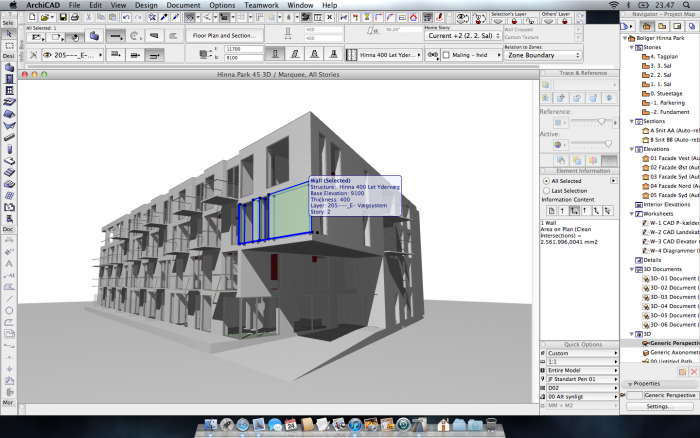
\includegraphics[width=0.48\textwidth]{./Images/Introduction/Example3DModellingTool_1.png}}%

\caption[General view of Traditional Design Approaches]{(a) Simplification of a computational design workflow (b) An example of a building design in a 3D modeling tool. Image retrieved from~\cite{3DMODELTOOL}}
\label{fig:traditionaldesign}
\end{figure*}

Shortly after, the development of computer-based simulation tools enabled designers to simulate the behavior of their designs regarding specific criteria, i.e., to get a measurement of the designs' performance~\cite{Malkawi2005}. Through this process, known as \ac{BPS}, designers can validate whether their design's performance satisfies the efficiency requirements and, ultimately, optimize the design by iteratively remodeling the geometry in order to obtain variations, assessing their performance, and selecting the better ones. Albeit still being very primitive, architects now have the elementary mechanisms required for optimizing their building's designs, which spurs a new \ac{PBD} approach: \ac{BPO}.

% #############################################################################
\subsection{Building Performance Optimization}

	\ac{BPO}, a simulation-based optimization approach, treats the results produced by simulation tools as the functions to optimize. Although suffering from some degree of imprecision and inaccuracy, these simulations make it possible to estimate the performance of complex designs. Particularly, these estimates are beneficial in designs for which analytical solutions are difficult or even impossible to derive~\cite{Kolda2003}. In these cases, the objective function, i.e., the function to optimize, is derived from the simulations' results. The domain of these functions corresponds to the range of acceptable designs,  which is specified by the architect.

	A known drawback of simulation-based approaches is the time required to achieve reasonable results for complex systems~\cite{Law1991}, which is associated with different aspects of the problem, namely: (1) its \textbf{domain} which, depending on the nature of the problem, might use different methodologies to produce the corresponding estimates (e.g., thermal \textit{versus} structural); (2) its \textbf{intrinsic structure} that, depending on the attributes and relations of the system, might lead either to simpler or to more complicated computations (e.g., skyscraper \textit{versus} a small house); and (3) its \textbf{analytical model}, i.e., a model containing the essential properties of the system we are trying to simulate and that will be used as input to the simulation tool. Generally, the domain and structure do not change for the same problem, however there are numerous ways to produce multiple analytical models. Depending on the level of detail of the analytical model, both the computational time and results of the simulation might change. 

	In architecture, the production of analytical models is a complex and tiresome task. On the one hand, it is often necessary to produce multiple analytical models of the same design because of the different simulation tools' specificities, i.e., each simulation tool requires its own specialized model of the same design. On the other hand, simulation is often a time-consuming process due to the amount of computation that is required.

% Motivation for other design alternatives
	Finally, a \ac{BPO} methodology requires the evaluation of different design variations, which, if done manually, implies spending a large amount of time with the application of changes to the design. Despite the flexibility provided by \ac{CAD} and \ac{BIM} tools, architects often face difficulties when modeling complex geometry. As a result, the whole optimization process becomes unviable.
	
% #############################################################################
\subsection{Algorithmic Design}
\label{ssec:ad}
% Introduction to AD, way of overcoming limitations of manual approaches
	A design approach capable of creating forms through algorithms is crucial for overcoming the aforementioned limitations. An example of such an approach is \ac{AD}~\cite{Branco2017AD} and \cref{fig:algorithmicdesign} illustrates a simplified scheme of its application in the architectural design workflow. In this approach, the architect develops an algorithmic description of the intended design, that, when executed, generates the corresponding 3D model in an architectural modeling tool, such as a \ac{CAD} or \ac{BIM} tool. Algorithmic approaches are inherently parametric, enabling the generation of different variations of the same design by simply modifying the parameters' values~\cite{Leitao2014GD}. 
	
\begin{figure}[htbp]
\centering

\includegraphics[width=0.70\textwidth]{./Images/Introduction/AlgorithmicArchitecturalDesign.png}
\caption[General view of the Algorithmic Design Approach]{Algorithmic Design workflow}
\label{fig:algorithmicdesign}
\end{figure}
	
	As an example, consider the algorithmic design of Astana's National Library by Bjarke Ingels Group (BIG) architects, illustrated in~\cref{fig:astana-a}. Since the library's shape resembles a \textit{möbius} strip, its algorithmic description is defined in terms of several parameters, amongst which the radius and the number of turns of the strip. Now, by invoking the algorithm with different values for these parameters, the architect can easily generate different variations of the building. \Cref{fig:astana-b,fig:astana-c} illustrate two design variations, where the radius and number of turns are increased, respectively.
	
\begin{figure*}[htbp]
\centering
\subfigure[]{%
\label{fig:astana-a}%
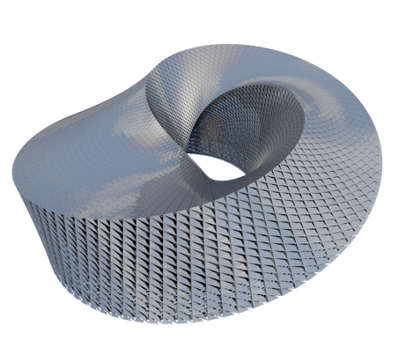
\includegraphics[width=0.32\textwidth]{./Images/Astana/Astana1.png}}%
\hfill
\subfigure[]{%
\label{fig:astana-b}%
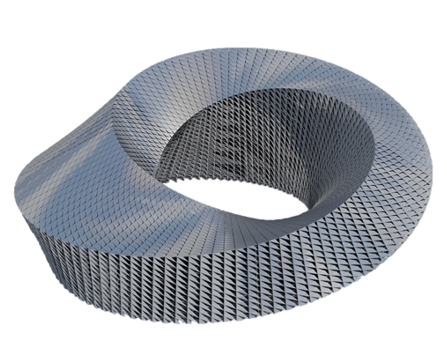
\includegraphics[width=0.33\textwidth]{./Images/Astana/Astana2.png}}%
\hfill
\subfigure[]{%
\label{fig:astana-c}%
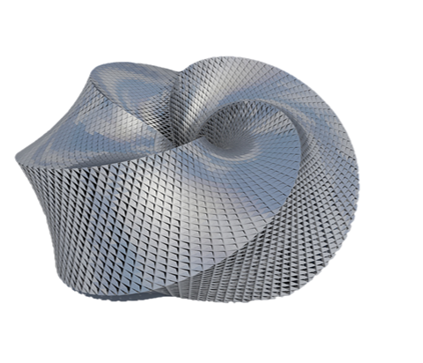
\includegraphics[width=0.33\textwidth]{./Images/Astana/Astana3.png}}%

\caption[Design variations of the Astana's National Library]{Design variations of the Astana National Library: (a) Original; (b) Larger diameter; (c) Two \textit{möbius} turns.}
\label{fig:astana}
\end{figure*}

% Advantages over Manual approaches & Disadvantages
Only recently has the algorithmic paradigm begun to settle in the architectural practice. The need for programming knowledge is often an obstacle to the adoption of this paradigm, since it requires a large initial investment for architects to learn such techniques. Despite these investments, the benefits arising from the use of algorithmic design approaches surpass those of directly using \ac{CAD} or \ac{BIM} tools to design complex buildings. Particularly, the initial investment is quickly recovered when the need for the incorporation of changes arises or when it becomes necessary to experiment different design variations. This is especially important when facing design processes that are characterized by constant changes to the project's constraints and requirements. In these scenarios, a manual-based approach requires constant manual changes to the model, thus incurring a dreadful and tiresome process, whereas an algorithmic approach enables the effortless generation of a broader range of design solutions, as well as the easy modification of the models to comply with new requirements. As a result, using \ac{AD}, architects are able to explore larger regions of the solution space, i.e., the set of possible design solutions, as well as innovative solutions that were not previously considered due to the time and effort required~\cite{Leitao2014GD}.

Another benefit of the \ac{AD} approach is the ease of maintenance of the models involved in building design. In fact, since \ac{AD} usually requires a single algorithmic description of the design, i.e., the algorithmic model, it is easier to maintain in scenarios where changes are frequent. On the other hand, manual-based-approaches often involve the creation and maintenance of multiple models of the same design (e.g., analytical models, 3D models), which quickly becomes hard and tiresome.

% Conclusion
The emergence of \ac{AD} was crucial for the automation of optimization processes by enabling the automatic generation of multiple design solutions. However, the optimization of these designs requires the creation of the corresponding analytical models, which can be very different from the 3D models originally produced by the \ac{AD} tool. Therefore, to evaluate the models produced by the \ac{AD} tool, the architect must manually generate the analytical model for each variation. Particularly, when dealing with complex buildings, this task requires a large amount of time and effort, which makes the optimization process almost impracticable.

% #############################################################################
\subsection{Algorithmic Analysis}
\label{ssec:aa}

% Motivação p/ passar de AD p/ AA.
Faster and broader design space exploration prompted the creation of increasingly complex building designs, which became less predictable with respect to different aspects~\cite{Branco2017AD}, such as thermal, lighting, acoustics, among others. Moreover, the recent focus on efficient and sustainable buildings led to the demand for buildings that, not only are well-designed, but also exhibit good performance in those aspects.
	
% Motivar necessidade de ferramentas de tradução de modelos 
Nowadays, most of the available simulation-based analysis tools are single-domain, each one evaluating the metrics that are specific of the domain~\cite{Malkawi2005}, i.e., while a lighting analysis tool measures daylight and glare coefficients, an energy simulation tool measures the coefficients related to thermal, energy consumption, ventilation, and air conditioning systems. Unfortunately, this often implies the production of different analytical models for each simulation tool. Moreover, the 3D models produced by the most common modeling tools are generally dissimilar to the specialized models required by each analysis tool. To evaluate the design performance regarding different domains (e.g., lighting, energy, structural), several analytical models have to be produced either by hand or through translation processes that convert generic 3D models into specialized models required for analysis.

% Motivar processos automáticos para tradução 
Unfortunately, the process of producing analytical models is still limited: (1) hand-made analytical models require a considerable amount of time and effort to create; (2) the existing tools that attempt to convert a 3D model into its corresponding analytical model are frequently fragile and can cause errors or loss of information; (3) when using the analysis results to guide changes in the original design, such changes require additional time and effort to implement, as does redoing the analysis to confirm the improvements. For these reasons, performance analyses are typically postponed to later stages of the design process, only to verify the fulfillment of the performance requirements.

To overcome the limitations associated with the production of analytical models, one can exploit the idea of using \ac{AD} to automatically generate analytical models from the 3D model's algorithmic description. \ac{AA} is an extension of the \ac{AD} approach that, besides enabling the automatic generation of analytical models from a design's algorithmic description, also automates the setup of the analysis tool and the collection of its results~\cite{Aguiar2017}. Using this approach, the architect creates the \ac{AD} model reflecting his design's intents and then sets a few configuration parameters according to the analysis tool to be used. \Cref{fig:algorithmicanalysis} illustrates both the \ac{AD} and \ac{AA} design workflows, as well as examples of the Astana National Library models produced in each tool. Note that, even though there is only one algorithmic description of the design, it is capable of producing very different models for each given tool. As an example, consider once more the Astana National library's façade, which is composed of a truss structure holding the photovoltaic panels that cover the building. This façade is represented by a set of masses illustrating the geometry of the building in a typical 3D model, by a graph of truss bars, nodes, and edges when submitted to structural analysis, and by triangulated surfaces topped with sensor nodes, in the case of lighting analysis.

 % the produced models can be very different, e.g., while a truss is represented by a set of masses illustrating its bars and nodes in a typical 3D model, it is represented by a graph of nodes and edges when submitted to a structural analysis, and, by its surfaces, in the case of a lighting analysis.

\begin{figure}[htbp]
\centering
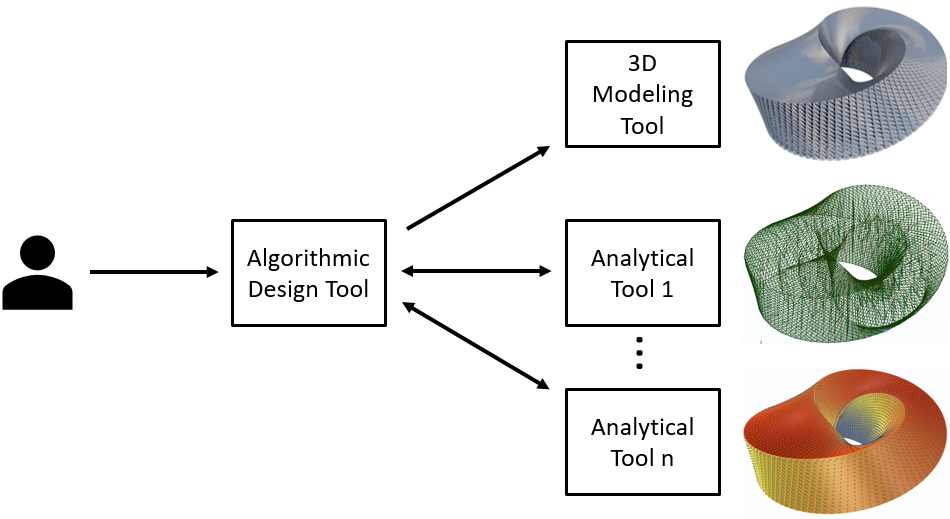
\includegraphics[width=1\textwidth]{./Images/Introduction/AlgorithmicDesignAndAnalysis_w_models2.png}
\caption[General view of the Algorithmic Design and Analysis approach]{\ac{AD} and \ac{AA} design workflow with examples of the Astana National Library design and analytical models: (top) 3D model; (center) structural analysis model (using Robot structural analysis tool); (bottom) pos-radiation analysis model (using Radiance analysis tool).}
\label{fig:algorithmicanalysis}
\end{figure}		
	
The \ac{AA} approach is able to enhance \ac{PBD} approaches, as it provides the means to effortlessly perform design analysis throughout the whole design process, instead of just at final stages. Depending on the performance requirements, architects might need to use different analysis tools: (1) for daylight analysis, Daysim and Radiance are very popular tools among the community, (2) for energy simulations, EnergyPlus, TRNSYS and DOE-2 are widely used~\cite{Nguyen2014}, (3) for structural analysis, Robot Structural Analysis and Tekla Structural Designer are well-known reputed tools, and (4) for acoustic analysis, Olive Tree Lab and Pachyderm Acoustical Simulation are examples of good tools.%~\cite{Branco2017AD}. 

Moreover, the \ac{AA} approach is also important for the automation of optimization processes, as it abstracts the production of the analytical model, removing the need for direct human intervention, while reducing the occurrence of errors and information loss. Additionally, when combined with \ac{AD}, it provides the required mechanisms to quickly update a design, to generate the corresponding analytical model, to automatically evaluate the design in an analytical tool, and, finally, to collect the results and use them to guide the search for optimal solutions. 

Despite the possibility of automating optimization processes, the lack of standardized approaches is an obstacle for its application within the architectural community~\cite{Attia2013}. In particular, to use such optimization processes, architects often need to acquire programming skills and invest large amounts of time and effort either to create their own optimization algorithm, to integrate dedicated optimization tools, or to include post-processing and visualization mechanisms to aid in the interpretation of the outcomes. As a result, architects rarely perform optimization or, when that is not the case, they tend to repeatedly use the same approach. While this is not always a disadvantage, it can have a negative impact in the overall optimization if, for example, architects apply inadequate algorithms over and over again.

Notwithstanding its obstacles, optimization prevailed and different approaches have spawned into the architectural practice. During this time, multiple surveys have identified the difficulties and the advantages of each approach, which enabled the development of optimization tools more targeted to architects' needs \cite{Attia2013,Nguyen2014,Shi2016}. In the following section, we briefly mention some of these approaches and we emphasize the key points of optimization processes in architecture.
	
% #############################################################################
\subsection{Architectural Optimization Workflow}
\label{ssec:AOW}
More recently, the emergence of \ac{AD} approaches based on visual programming, such as Grasshopper and Dynamo~\cite{GRASSHOPPER,DYNAMOBIM}, together with the growing consciousness of both the benefits and limitations of optimizing building designs, led to the development of ready-to-use optimization toolsets (e.g., Galapagos and Opossum). Even though the combination of visual programming and optimization tools allowed architects to perform design optimization, architects can rarely apply it to more complex designs due to the scalability limitations generally associated with this programming paradigm~\cite{Heijden2015}.

On the other hand, \ac{AD} approaches based on textual programming techniques are known to scale better with design complexity. In addition to the scalability benefits, its growing popularity among building design practitioners~\cite{Kestelier2013}, its flexibility and its capacity to automate optimization processes allow the development of more robust and complete optimization tools. To fully benefit from these properties, the architect must follow an optimization methodology based in \ac{AD}, where he first idealizes a design and then creates the corresponding algorithmic program by defining the parameters that represent the degrees of freedom of the design, i.e., the parameters that he is willing to manipulate. Using the design's algorithmic definition, the \ac{AD} tool generates either a 3D or an analytical model for visualization and performance analysis purposes, respectively. Optionally, the architect may decide to optimize his design according to some particular performance aspects (e.g., lighting, energy consumption, cost), potentially leading to the exploration of design solutions that were not previously considered. In that case, the optimization algorithm explores different design candidates, using the results produced by the simulation tools as the functions to optimize. The execution of the optimization algorithm then yields optimal (or near optimal) design solutions.

Considering the previous view of an algorithmic-based design workflow, we identify four key aspects in an optimization process:

% ------- BEGIN \ --------
\begin{enumerate}
% ANALYTICAL MODELS
\item \textbf{Analytical models}: when the optimization algorithm specifies a candidate design, i.e., a concrete configuration for the parameters of the model, analytical models are automatically generated by the \ac{AD} tool and then used as input for the corresponding analysis tools. These models can be improved either through simplification of the analytical models or by enriching them with context information. The former enables the simplification of the analysis itself by providing an equivalent but simpler model to the tool, potentially reducing the simulation time, whilst the latter enables the attainment of more detailed and realistic simulations, which is not always possible due to limitations in the \ac{AD} tool. 

% OPTIMIZATION ALGORITHM
\item \textbf{Optimization algorithms}: the algorithms used to explore the design space in the quest for optimal (or near optimal) solutions. These algorithms use the results obtained in the performance analysis of different design variations as the functions to optimize, i.e., objective functions. %Generally, optimization algorithms use the inferred functions to guide the search for optimal solutions. 
The algorithm's time complexity typically depends on the number of times these functions are evaluated. In architectural design, these functions entail time-intensive simulations, which implies highly time-consuming optimization processes.

% EXPLAINABILITY / INTELLIGIBILITY OF RESULTS
\item \textbf{Intelligibility of results}: the ability to interpret and understand the design optimization results is very important within the architectural community \cite{Shi2016,Cichocka2017SURVEY}. Having access to an explanation regarding the quality of a solution allows architects to make more informed design decisions. In this way, not only can the architect provide valuable arguments for its implementation, but he can also learn with the process, depending on the quality of the explanations, thus fostering more efficient and faster future designs. 

% INTERACTIVITY AND VISUALIZATION
\item \textbf{Interactivity and visualization}: interactive and visual aspects are highly important features in the context of optimization processes~\cite{Ashour2015CreativelyMOO}. On the one hand, an interactive optimization process enables the architect to use knowledge about the problem at hand, for instance, by adding or removing constraints or by exploring different, yet unexplored regions of the design space, hence potentially increasing the process' performance. On the other hand, optimization processes providing better visualizations and representations of their own evolution can present their users with better feedback about the course of the search. This feedback is important to the comparison of variable-objective correlations and the making of more informed design decisions about the optimization process itself, e.g., whether the evaluations made so far suffice or if the algorithm is converging to non-conventional designs that diverge from the original design intent.
\end{enumerate}

% #############################################################################
\section{Dissertation Goals}
\label{sec:goals}

This dissertation focuses on optimization problems involving expensive evaluation functions, namely, in the context of building design. Despite the evident benefits of architectural design optimization, its application within the architectural community remains infrequent. This might be explained by its considerable time complexity that goes against the time sensitiveness of most design practices~\cite{Shi2016}. Time becomes an even greater impediment when it is necessary to evaluate multiple performance aspects, instead of a single one, as it frequently happens in building design. In this case, it is of paramount importance that the optimization algorithms used are capable of efficiently handling problems involving expensive evaluation functions. Unfortunately, the currently available architectural optimization tools do not, in general, provide good algorithms for handling such problems.

This dissertation sets out to address this problem, by identifying the most adequate algorithms for optimizing computationally complex problems and exploring their application to architectural design. In this research, we consider not only building design problems involving a single performance aspect, i.e., \ac{SOO}, but also the optimization of multiple aspects simultaneously, that is, \ac{MOO}. Based on the idea that no algorithm can consistently perform better than the others on all problems~\cite{Wolpert1997NFLT}, this dissertation explores this performance difference by studying algorithms with different properties. 

The main goal of this dissertation is to identify the most efficient optimization algorithms for the different performance optimization problems that occur in building design and that frequently involve computationally heavy evaluation functions. Moreover, this dissertation aims to encapsulate these algorithms in an optimization framework that simplifies their application and, thus, promotes design optimization in architecture. Finally, we evaluate the proposed framework in the architectural practice and we study the behavior of different algorithms in various real \ac{BPO} problems, including the optimization of simulation-based lighting, structural, and cost aspects of buildings. 

% #############################################################################
\section{Document Structure}
The following chapters are organized as follows:
\begin{itemize}
% \textbf{\Cref{chap:intro}} discusses optimization concepts and evidences its importance for different problems, ranging from simple day-to-day decisions to more complex engineering problems, such as components, circuits, and building designs. Particularly, this chapter stresses the relevance of optimization in the architectural context, providing a comprehensive overview of the existing practices and the difficulties underlying the adoption of optimization processes in architecture. \\
\item \textbf{\Cref{chap:back}} presents an overview of the current optimization practices in architecture and compares the benefits and drawbacks associated with each one.  
\item \textbf{\Cref{chap:architecture}} describes the proposed framework and enumerates important design decisions that were made during its implementation. 
\item \textbf{\Cref{chap:implement}} describes the application of the proposed framework to the architectural practice. 
\item \textbf{\Cref{chap:evaluation}} analyzes both qualitative and quantitative aspects of the proposed framework, comparing it with currently existing architectural optimization tools and evaluating multiple optimization algorithms in the context of three case studies.
\item \textbf{\Cref{chap:conclusion}} emphasizes the importance of optimization in architecture and draws some conclusions about this work and how it can influence the architectural practice. Finally, we reflect on the future improvements for the proposed framework.
\end{itemize}

% emphasizes the importance of optimization in architecture, compares the proposed framework with the currently existing architectural optimization tools, and draws some conclusions regarding the suitability of the studied algorithms. % for handling design problems that involve expensive objective functions. Moreover, it discusses the impacts of this dissertation and how it benefits the architectural practice. Finally, we reflect on the future improvements for the proposed framework. \\

% If Printing on DOUBLE SIDED pages, the second page should be white.
% Otherwise, comment the following command:
\cleardoublepage
%
%Chapter 2
% #############################################################################
% This is Chapter 2
% !TEX root = ../main.tex
% #############################################################################
% Change the Name of the Chapter i the following line
\fancychapter{Background}
\cleardoublepage
% The following line allows to ref this chapter
\label{chap:back}

	The development of an algorithmic-based framework for optimization, applicable to architectural domains, requires a careful review over the current literature on \ac{BPO} practices and their limitations. 
	
	Firstly, building design is a multi-disciplinary practice that involves a wide variety of different problems. According to their characteristics, some optimization algorithms may be more or less adequate to address them, as algorithms often adopt different strategies or techniques. To maximize the potential of the optimization, it is therefore necessary to distinguish between different problems and which optimization algorithms are more suitable for which problems. One important distinction is between single- and multi-objective problems. Generally, \ac{BPO} practices require the optimization of multiple aspects simultaneously, a multi-objective problem. However, this objectives' multiplicity instills performance issues that must be properly addressed. This chapter discusses four different approaches to address these problems.
	
	Secondly, the costly nature of the functions used for performance assessment in \ac{BPO} motivates the application of a special class of optimization algorithms, the derivative-free algorithms. Within this class, different categories emerge, emphasizing the algorithms' different properties and search strategies. Applying the adequate algorithm to certain problems may potentially increase the efficiency of optimization processes, especially for problems involving time-consuming evaluations.
	
	Finally, the development of design optimization tools fostered the coupling between optimization and design practices. Currently available architectural optimization tools optimize the parametric models produced in the visual programming environments, like Grasshopper and Dynamo. These environments are closely integrated within \ac{CAD} and \ac{BIM} tools, respectively, hence enabling a seamless and friendlier association between optimization tools and typical \ac{BPO} design workflows. Also, the \textit{ready-to-use} format of these optimization tools' interfaces are very appealing to most \ac{BPO} practitioners~\cite{Cichocka2017SURVEY}.
	
	After a comprehensive description of the previously mentioned views of \ac{BPO} practices, in \Cref{sec:problemsaddress}, we emphasize the main limitations of currently existing \ac{BPO} practices. 
	
\section{Optimization Problems}
\label{sec:optimizationproblems}
	
	Generally, an optimization process consists in two main parts: modeling and optimization algorithms. Covered in this section, the first part involves the creation of a model representing the system or problem to optimize, while the second part, further discussed in \Cref{sec:optimizationalgorithms}, focus on the application of a strategy capable of searching among the set of possible solutions, i.e., the solution space, for optimal solutions.
	
	An optimization process often starts with the formulation of the model of the system or problem to address, in a process known as modeling. The model is described in terms of (a) the variables or unknowns, which represent the system's or problem's characteristics, (b) the objectives or criteria, representing the quantitative measures of the system's performance, which are usually functions of the variables, and, optionally, (c) the constraints, representing the conditions that have to be satisfied to guarantee the system's feasibility~\cite{Nocedal2011NumericalOptimization}. 
		
	There are numerous possibilities to create optimization models, each yielding a different mathematical classification. Concretely, models variability include, among others, the variable types, the presence or absence of constraints, and the number and nature of the objective functions. In addition to the model, the search strategies can also be classified according to the scope of the search, i.e., whether they explore vaster or narrower regions of the solution space. 
	
	Particularly, in \ac{BPO}, building designs may yield different optimization problems, depending on the way they are modeled and the limitations or restrictions imposed by architects or engineers. For example, in order to reduce fabrication costs it is very frequent to limit the granularity of the design's components to vary within certain values. As another example, consider the situation where, to preserve the architect's intention, building designs are confined to have specific shapes (e.g., arc-shaped, round-shaped, squared-shaped) and each shape can be varied according to some defined parameters. Moreover, it is also possible that when building design becomes more complex, architects decide to relax some of the previously established conditions. Indeed, as it will be further discussed in \Cref{ssec:soo,ssec:preferencesarticulation}, when facing problems involving the simultaneous expensive evaluation of multiple performance aspects, time restrictions often force architects to abdicate some performance aspects, or, in some cases, to define a preference amongst the considered performance aspects.
	
	
\subsection{Problems Classification}
	
	The mathematical optimization field offers different classifications for optimization problems. In this chapter, we introduce three of these classifications due to their relevance and their ubiquitousness for optimization problems. \Cref{fig:optclassification} exhibits a schematic representation of the four different optimization classifications considered in this dissertation (the fourth classification will be discussed in \Cref{sec:optimizationalgorithms}). For a more comprehensive treatment of this subject, consider~\cite{Nemhauser1988,Nocedal2011NumericalOptimization}. 
	 
	The first classification differentiates \textbf{continuous} and \textbf{discrete} optimization problems depending on the variables' types. Continuous optimization refers to problems defined uniquely by continuous variables and, therefore, characterized by an infinite solution space, whereas discrete optimization refers to problems for which some or all their variables are discrete, hence yielding a finite solution space. In continuous optimization, the smoothness of functions make it possible to reason about the behavior of all points close to $x$ and, consequently, to solve these problems more easily, whilst the commonly present irregularities of discrete optimization functions do not, in general, allow to draw any information about the behavior of points close to $x$. Discrete classification encloses finer optimization classes, such as integer optimization or combinatorial optimization~\cite{Nemhauser1988}. 
	
	The second classification relates to the presence of constraints on the variables. \textbf{Unconstrained} optimization problems result from many practical applications and have no restrictions on the variables' values. Contrastingly, \textbf{constrained} optimization problems usually emerge from systems where constraints are crucial (e.g., economy problems, imposing cargo constraints) and are incorporated them into the problem's definition. Variables can be restricted using hard or soft constraints. Hard constraints set conditions for the variables that must be satisfied, namely, to vary within simple bounds (e.g.: $-1<x<1$) and to relate to other variables in certain ways (e.g.: $\sum_{i} x_i$), whereas soft constraints set penalties for the variables whose value violates the condition. Constrained optimization problems are often converted to unconstrained ones by replacing hard constraints with soft constraints, i.e., by adding penalization terms in the objective function to discourage the violation of constraints~\cite{Nocedal2011NumericalOptimization}. 

	The third, and final, dichotomy herein discussed focuses on the number of objectives to optimize, which can be distinguished in \textbf{single-objective} and \textbf{multi-objective}. \ac{SOO} focus on the optimization of one objective, whilst \ac{MOO} focus on problems involving multiple conflicting objectives simultaneously. Besides the larger objectives' number, addressing multi-objective problems also entails more complex optimization problems. For problems involving time-consuming evaluations, the increased complexity jeopardizes the executability of optimization and spurs the adoption of other, often simpler, approaches. The following sections describe different approaches to single- and multi-objective optimization problems. 
	
	\todo{Put picture with the scheme - make in ppt}
	\begin{figure}
		\centering
		
\includegraphics[width=5cm]{Images/placeholder-image.png}
		\caption{Different classifications of optimization processes.}
		\label{fig:optclassification}
	\end{figure}
	
	% ----------- 
	\subsection{Design of Experiments}
	\label{ssec:doe}
	
	The experimental or design of experiments approach is widely used in research and in practice to address both single and multi-objective problems~\cite{Fang2017}. Besides being intuitive and flexible, it can achieve a potentially better solution without having to deal with complex optimization algorithms. This approach evaluates designs generated with different combinations of design parameters. These combinations can be obtained through sampling methods, such as Full-factorial, Monte Carlo Sampling, or Latin Hypercube Sampling~\cite{Giunta2003DOE}, which generate different variations of the design to be evaluated. This approach returns multiple design solutions instead of just one, leaving the final choice in the hands of the architect.
	
	Unfortunately, this approach does not guarantee that good solutions will be found. In fact, in most cases, new solutions are generated without taking advantage of the information obtained from previously evaluated designs. Consequently, the old information is not used to guide the search towards the most efficient designs and useless candidate designs can sometimes be evaluated. 
	
	On the other hand, given its simplicity and flexibility, this approach allows architects to easily combine different processes in order to direct the search towards better design solutions. For example, the architect can choose a sampling method to generate different design variations, which are then evaluated. After analyzing the results of the evaluations, the architect may wish to explore regions of the design space near the most promising design solutions. In that case, he might constrain the design variations to lie within the promising regions, by updating the problem’s definition. The redefined problem is then subsequently sampled and redefined until the architect is satisfied with the quality of the obtained solutions.
	
	Despite the constant need for manual intervention, the previous technique can be adapted to automatically extract information about the design problem itself, for example, to study the impact of design parameters in the performance. This process, commonly known as \textit{sensitivity analysis}~\cite{Saltelli2007}, has already been applied in the context of building design optimization~\cite{Tian2013}, not only to achieve better solutions, but also to enhance the performance of existing optimization algorithms, e.g., by dropping irrelevant parameters.
	
	Overall, while it does not provide guarantees about the solutions’ optimality, this approach is simple, easy to use, and it is available in numerous tools. Moreover, although this process is not intelligent \textit{per si}, since the decisions are always made by the architect, it enables a more informed design process, as it presents all the design variations generated and their associated performance.
	
	% #############################################################################
	\subsection{Single-Objective Optimization}
	\label{ssec:soo}
	
	\ac{SOO} processes aim to find the best solution with respect to a unique objective function. This function is described in terms of the values of the problem's parameters. \Cref{eq:soo} illustrates an example of a mathematical constrained minimization \ac{SOO} problem, where $f$ represents the single-objective function, $g_j$ and $h_k$ represent the constraints to be satisfied, and $x$ represents the parameters' vector.
	
	\begin{equation} \label{eq:soo}
	\begin{aligned}
	& \underset{x \in \mathbb{R}^n}{\text{minimize}}
	& & f(x) \\
	& \text{subject to}
	& & g_j(x) = 0, & \; j &= 1, \ldots, J, \\ 
	&&& h_k(x) < 0, & \; k &= 1, \ldots, K.
	\end{aligned}
	\end{equation}
	
	Generally, the computational complexity of optimization processes is exponential on the number of objectives and, consequently, the more objectives, the more expensive processes are. In particular, \ac{SOO} processes rely exclusively on a single objective function and are, therefore, usually less time-consuming than \ac{MOO} processes. The main difference between these two processes is that the former focus on finding the solution that optimizes a single function, whereas the latter focus on finding the optimal trade-offs between the, potentially conflicting, multiple objective functions. The difference in the computational resources become particularly relevant when considering simulation-based objective functions, as these tend to be very time-consuming. 
	
	Particularly, in the case of building design, because most problems include simulation-based objective functions, architects commonly opt for \ac{SOO} processes~\cite{Wortmann2017Opossum}: either by simply considering a single performance aspect (or objective), or, in the case of problems involving multiple conflicting aspects, by combining them in a unique function as it will be further explained in \cref{ssec:preferencesarticulation}.
	
	A literature review over the architectural practice will evidence the prevalence of \ac{SOO} practices. Firstly, single-objective problems are easier to model. Secondly, available optimization plug-ins, like Galapagos and Goat, allow to easily address single-objective building design problems. As a result, not only are architects capable of solving these optimization problems, but, when facing more complex \ac{MOO} problems, they are also encouraged to adopt simplified versions of such problems, thus reducing the overall complexity of those optimization processes. Finally, the variety of optimization algorithms exposed in these plug-ins enables the selection of the best algorithm to specific problems, thus spurring more efficient optimization processes~\cite{Wortmann2016BBO}.  
	
	Although \ac{SOO} yields less time-consuming processes, these are also less informative than \ac{MOO}, as they usually focus on a single optimal solution. As a case in point, building design often involve different conflicting aspects (e.g., thermal, energy consumption, cost), for which information about the different compromises would aid in the comprehension and making of more informed decisions.
	
	% #############################################################################
	\subsection{\textit{A Priori} Articulation of Preferences}
	\label{ssec:preferencesarticulation}
	
	This approach comprises a simplified way of handling \ac{MOO} that is very resemblant of the \ac{SOO} approach previously discussed, but without disregarding any of the performance aspects. Particularly, this approach combines multiple objective functions according to one’s preferences, using what is called a utility function \cite{Marler2004}, i.e., a function which ranks alternatives according to their utility for global performance. 
	
	Among all the possible utility functions, the most common one is the weighted sum~\cite{Wortmann2017Opossum}, also referred to as linear \textit{scalarization}, in the literature. This utility function reduces \ac{MOO} to \ac{SOO} problems by weighting the different objectives and combining them into a single function, as depicted in~\Cref{eq:scalarization}. The weights ($w_i$) assigned to each objective function ($f_i$) represent their relative importance to the architect and they must be set during the modeling of the optimization problem, that is, before starting the search for optimal solutions. The resulting function is then provided to a \ac{SOO} algorithm as the function to optimize. 
	
	\begin{equation} \label{eq:scalarization}
	\begin{aligned}
	& \underset{x \in \mathbb{R}^n}{\text{minimize}}
	& & \sum_{i=1}^n w_i f_i(x), & \; i &= 1, \ldots, n, \\
	& \text{subject to}
	& & g_j(x) = 0, & \; j &= 1, \ldots, J, \\ 
	&&& h_k(x) < 0, & \; k &= 1, \ldots, K.
	\end{aligned}
	\end{equation}
	
	Despite its similarity to \ac{SOO}, this approach incurs into a much more computationally complex process than the latter one, as it still involves the evaluation of multiple objective functions. As a result, the time complexity process is considerably increased and, instead of taking seconds, minutes, hours, or days, per function evaluation, takes that value multiplied by the number of objectives. Nevertheless, this approach still manages to be less time-consuming than the analogous Pareto-based \ac{MOO} approach (that will be discussed in \Cref{ssec:pareto}), as it focus on the optimization of a single preference, instead of attempting to find the trade-offs among all the objectives. 
	
	As a case in point, in architecture, this approach is particularly useful, when more experienced architects can use additional knowledge to define an appropriate set of preferences, instead of resorting to the analogous Pareto-based approach, which would yield a far more complex optimization process. In terms of the impacts in the design process itself, this approach yields a more intelligent, but less informed design process. On the one hand, it confers intelligence because the involved optimization algorithms usually exploit the knowledge of previously evaluated solutions to guide the search towards optimal regions of the design space. On the other hand, it is less informed, because architects no longer control or have information about the optimization process. The loss of control results from the automated character of the optimization algorithms involved in the architectural practice, which frequently exclude architects from the optimization loop. As a consequence, in general, the architect has no information about the solutions evaluated during the optimization process and is only provided with a single solution\footnote{The interest in having a subset of optimal solutions led to the development of mechanisms to provide a subset of optimal solutions instead of a single one.}. The lack of information is perceived as a limitation ~\cite{Cichocka2017SURVEY} and it restricts the architect to either comply with the retrieved solution or to rerun the optimization again. Either way, this optimization approach does not provide in general enough information to understand the optimization results, and, consequently, make more informed decisions. 
	
	Overall, in architectural domains, the virtues of this approach include the ease of use, the availability, the heterogeneity of ready-to-use \ac{SOO} tools (e.g., Opossum, Goat, Galapagos, Silvereye), and the time complexity. %when compared to other \ac{MOO} approaches. % In general, because this preference-based approach focus in the retrieval of a single optimal solution that satisfies the previously defined preferences, it becomes more effective and less time consuming than other \ac{MOO} approaches, that either lack a more guided search or that aim at finding solutions that are optimal under different preference articulations. 
	
	% #############################################################################
	\subsection{Pareto-based Optimization}
	\label{ssec:pareto}
	
	Despite allowing to handle \ac{MOO} problems, the previous approach does not consider the different trade-offs among the potentially conflicting objectives, instead forcing the user to make an \textit{a priori} decision regarding the importance of each objective. Pareto-based optimization approaches attempt to address this limitation by postponing that decision until the end of the optimization process. In this approach, all objectives are taken as equally important during the optimization, making it more difficult to discern the quality of each solution. In other words, while in \ac{SOO} problems, we expect the optimal solution to be the set of parameters' values that achieve the best\footnote{For simplification purposes, we simply refer to the optimal solution as being the best. When dealing with a minimization problem, the best solution is the one that achieves the lowest value of the objective function, whereas in maximization problems, the best solution is the one achieving the highest value of the objective function.} objective value possible, in \ac{MOO}, the best possible configuration for one of the objectives is rarely the best possible configuration for all other objectives, which results from the fact that these objectives are often contradictory. \Cref{eq:pareto-based} presents an example of the mathematical definition of a constrained minimization \ac{MOO} problem, where $F(x)$ represents the vector of $k$ objectives, $f_i$ represent the $i^{th}$ objective function, $g_j$ and $h_k$ represent the constraints to be satisfied, and $x$ represents the parameters' vector.
	
	
	\begin{equation} \label{eq:pareto-based}
	\begin{aligned}
	& \underset{x \in \mathbb{R}^n}{\text{minimize}}
	& & \left\lbrace F(x) = \left[f_1(x), f_2(x), ..., f_n(x)\right]  \right\rbrace \\
	& \text{subject to}
	& & g_j(x) = 0, & \; j &= 1, \ldots, J, \\ 
	&&& h_k(x) < 0, & \; k &= 1, \ldots, K.
	\end{aligned}
	\end{equation}
	
	In order to assess the quality of multi-objective solutions, it becomes necessary to apply a new optimality criterium, like the Pareto optimal (or Pareto efficient) concept. Named after the economist Vilfredo Pareto, the Pareto optimal concept defines an optimal solution as being a solution for which it is impossible to improve an objective value without deteriorating others. Such a solution is also said to be non-dominated or noninferior, and the set of non-dominated solutions is called the Pareto front. An example of a bi-objective minimization problem is illustrated in \Cref{fig:paretofrontier}. The two objectives are $f_1$ and $f_2$, and the solutions shown in orange are non-dominated. The goal of Pareto-based optimization algorithms is to find design solutions that lie on the Pareto front.
	
	% Begin Pareto-Optimization Figure -------------------------------------------------------
	\begin{figure}
		\centering
		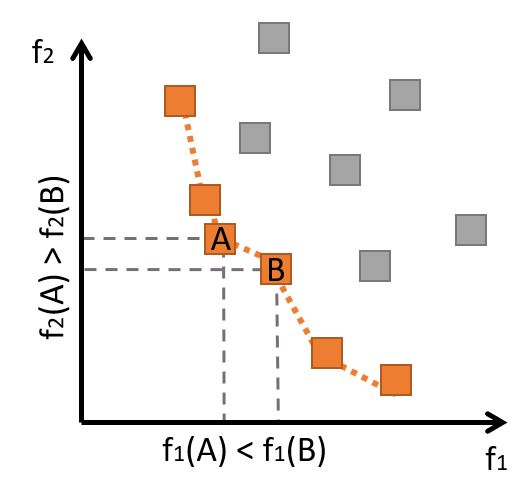
\includegraphics[width=5cm]{Images/Background/pareto-front.JPG}
		\caption[Representation of a Pareto front example for a bi-objective optimization problem]{Representation of the set of non-dominated (orange squares) and dominated (gray squares) solutions for a two-objective minimization problem. The Pareto front is composed of all the non-dominated solutions.}
		\label{fig:paretofrontier}
	\end{figure}
	% End Figure -------------------------------------------------------
	
	When considering the architectural practice, building design is a complex task that frequently involves dealing with multiple conflicting objectives, such as maximum lighting comfort \textit{versus} maximum thermal comfort, or minimum energy consumption \textit{versus} maximum thermal comfort. Even though the three previous approaches provide enough mechanisms for handling \ac{MOO} problems, they lack a more guided and informative strategy capable of retrieving a diverse and representative set of different trade-offs between the various performance aspects, i.e., the objective functions.
	
	Alternatively, the Pareto-based optimization approach provides the user with the set of non-dominated solutions that represent the different conflicts or trade-offs between the considered objectives. When confronted with this set of solutions, architects can compare the different design options, according to different performance criteria, and, thus, make more informed decisions about the different compromises involved. 
	
	On the other hand, in this approach, (1) the number of function evaluations is larger due to the need to find a set of optimal solutions instead of focusing on a single one, (2) the visual representation of the solutions’ objectives values becomes problematic when the number of objectives is greater than three, and (3) the way the optimization problem is modeled has a direct impact on the quality of the solutions.
	
	% #############################################################################
	
	\subsection{Comparison}
	\todo{Organizar tabela de forma mais lógica... O texto também...}
	
	This section focus on the comparison of the previously mentioned approaches, for which \Cref{table:optimization-approaches} provides a summarized view.
	
	\todo{Put column DoE before the SOO}
	\begin{table}[]
		\centering
		\resizebox{\textwidth}{!}{%
			\begin{tabular}{l|l|l|l|l|}
				\cline{2-5}
				& \multicolumn{1}{c|}{\begin{tabular}[c]{@{}c@{}}Single-objective \\ optimization\end{tabular}} & \multicolumn{1}{c|}{\begin{tabular}[c]{@{}c@{}}A priori preference \\ articulation\end{tabular}} & \multicolumn{1}{c|}{\begin{tabular}[c]{@{}c@{}}Pareto-based \\ optimization\end{tabular}} & \multicolumn{1}{c|}{\begin{tabular}[c]{@{}c@{}}Design of \\ experiments\end{tabular}} \\ \hline
				\multicolumn{1}{|l|}{Fundamentals} & \multirow{2}{*}{\begin{tabular}[c]{@{}l@{}}Maximization / \\ minimization\end{tabular}} & \multirow{2}{*}{Preferences} & \multirow{2}{*}{Pareto Front} & \multirow{2}{*}{Sampling} \\
				\multicolumn{1}{|l|}{} &  &  &  &  \\ \hline
				\multicolumn{1}{|l|}{Manual intervention} & \multirow{2}{*}{None} & \multirow{2}{*}{\begin{tabular}[c]{@{}l@{}}Preferences definition \\ (a priori)\end{tabular}} & \multirow{2}{*}{\begin{tabular}[c]{@{}l@{}}Preferences definition \\ (a posteriori)\end{tabular}} & \multirow{2}{*}{Constant} \\
				\multicolumn{1}{|l|}{} &  &  &  &  \\ \hline
				\multicolumn{1}{|l|}{Optimal solutions} & \multirow{2}{*}{Maximal / Minimal} & \multirow{2}{*}{Utility-based} & \multirow{2}{*}{Pareto optimal} & \multirow{2}{*}{Any} \\
				\multicolumn{1}{|l|}{} &  &  &  &  \\ \hline
				\multicolumn{1}{|l|}{Number of optima} & \multirow{2}{*}{1} & \multirow{2}{*}{1} & \multirow{2}{*}{1+} & \multirow{2}{*}{Unknown} \\
				\multicolumn{1}{|l|}{} &  &  &  &  \\ \hline
				\multicolumn{1}{|l|}{Provided information} & \multirow{2}{*}{Best solution} & \multirow{2}{*}{Best solution} & \multirow{2}{*}{Optimal solutions} & \multirow{2}{*}{Evaluated solutions} \\
				\multicolumn{1}{|l|}{} &  &  &  &  \\ \hline
				\multicolumn{1}{|l|}{Time Complexity} & \multirow{2}{*}{++} & \multirow{2}{*}{+++} & \multirow{2}{*}{+++++} & \multirow{2}{*}{+} \\
				\multicolumn{1}{|l|}{} &  &  &  &  \\ \hline
				\multicolumn{1}{|l|}{Configurable in process} & \multirow{2}{*}{Nothing} & \multirow{2}{*}{Preferences} & \multirow{2}{*}{Nothing} & \multirow{2}{*}{All} \\
				\multicolumn{1}{|l|}{} &  &  &  &  \\ \hline
				\multicolumn{1}{|l|}{Ease of use} & \multirow{2}{*}{+++} & \multirow{2}{*}{++} & \multirow{2}{*}{+} & \multirow{2}{*}{+++} \\
				\multicolumn{1}{|l|}{} &  &  &  &  \\ \hline
				\multicolumn{1}{|l|}{Ease of comprehension} & \multirow{2}{*}{Difficult} & \multirow{2}{*}{Difficult} & \multirow{2}{*}{Accessible} & \multirow{2}{*}{Easy} \\
				\multicolumn{1}{|l|}{} &  &  &  &  \\ \hline
				\multicolumn{1}{|l|}{Support in architecture} & \multirow{2}{*}{++} & \multirow{2}{*}{++} & \multirow{2}{*}{+} & \multirow{2}{*}{+++} \\
				\multicolumn{1}{|l|}{} &  &  &  &  \\ \hline
				\multicolumn{1}{|l|}{Main advantages} & \multirow{2}{*}{Time complexity} & \multirow{2}{*}{\begin{tabular}[c]{@{}l@{}}Search guided \\ towards a single objective\end{tabular}} & \multirow{2}{*}{\begin{tabular}[c]{@{}l@{}}Obtain different \\ trade-offs\end{tabular}} & \multirow{2}{*}{Full control} \\
				\multicolumn{1}{|l|}{} &  &  &  &  \\ \hline
				\multicolumn{1}{|l|}{Main Disadvantages} & \multirow{2}{*}{Lack of information} & \multirow{2}{*}{Lack of information} & Time complexity & Manual intervention \\
				\multicolumn{1}{|l|}{} &  &  & Results representation & No optima guarantees \\ \hline
			\end{tabular}%
		}
		\caption{Comparison between different optimization approaches}
		\label{table:optimization-approaches}
	\end{table}
	
	On the one hand, in terms of manual intervention, the design of experiments approach confers higher levels of control at the cost of constant manual intervetion (e.g., number of variations to generate, number of iterations to run sampling methods, choice of optimal solutions). The same does not happen with other approaches for which intervention is residual or even inexistent.	
	
	On the other hand, with higher control levels, the user gains more insight about the optimization process. Concretely, when following a design of experiments approach, the user is provided with all the information about all the solutions that were evaluated during the optimization process, whereas in the other approaches the user is only provided with the optimal solutions. The availability of information has a direct impact in the ability to comprehend the optimization results.
	
	The automation of optimization processes prompts the need for automatically evaluating the quality of solutions, thus requiring some optimality concepts: (1) depending on whether it is a maximization or a minimization problem, the \ac{SOO} approach considers the best solution to be the one presenting the largest or smallest value, respectively; (2) the \textit{a priori} preference of articulations approach applys a similar criteria, but it first entails the definition of a utility function to reduce a \ac{MOO} to a \ac{SOO} problem; and (3) the Pareto-based optimization approach is based on the Pareto optimality, leaving the final decision about the optimal solutions to the user.
	
	Depending on the approach, the solution's number and quality may vary. In general, all but the design of experiments approach presents a guided and, thus, more intelligent strategy to seek for efficient solutions. As a result, this approach does not guarantee that good solutions are found. Conversely, the other approaches tend to yield one or more optimal (or near) optimal solutions depending on whether it is a Pareto-based approach or not.
	
	A crucial point to take into consideration is the time difference between each approach, with the Pareto-based and the design of experiments approaches being the most and the less time-consuming, respectively. The former one requires searching the solution in space with the aim of finding the best trade-offs between different objectives, whereas the latter simply relies on a sampling strategy which generates different paramters' variations to be evaluated. This time difference is particularly concerning in the case of problems with costly evaluation functions, as it is the case of building design. Even though the \textit{a priori} preference-based approach involves the same objectives as the analogous Pareto one, it can be considerably faster. This results from the fact that this approach focus on the satisfiability of a certain set of preferences, instead of exploring a wider set of solutions.
	
	Indeed, when shifting to architecture, Pareto-based approaches are less applied in practice. Nevertheless, a few studies concerning this optimization approach have emerged in the past years, evidencing its utility~\cite{Evins2013,Hamdy2016}. Additionally, recent works show that despite the lower time complexity of \ac{SOO}-based and \textit{a priori} preference-based approaches, they are not as desirable as the Pareto-based ones~\cite{Attia2013,Cichocka2017SURVEY}. In fact, the latter ones enhance the decision making process, providing a clear insight about the trade-offs between the objectives involved. %Moreover, these multiple compromises represent different articulation of preferences from which the architect selects one. This approach is also called \textit{a posteriori} articulation of preferences.

	Despite the relevance and growing interest of Pareto-based optimization approaches, the lack of relevant benchmarks comparing the performance of different algorithms in the architectural field is evident. 


	\todo{Ease this transition...}Each optimization approach comprises different optimization algorithms. In the particular case of building design, the nature of the costly evaluation functions not only directly influences the overall optimization time, but also the algorithms' nature, as it will be discussed in the next section. 
	

% ##########################################################################
% ##########################################################################
% ##########################################################################
\section{Optimization Algorithms}
\label{sec:optimizationalgorithms}
	
	We have said that optimization processes are comprised by two parts: the first one, described previously, focused on the modeling of the problem and, a second one, which involves exploring the optimization model with the aim of finding more efficient solutions. This exploration part is achieved by means of optimization algorithms and will be the focus of this section. 
	
	Optimization algorithms search for the optimal solutions among the set of all possible solutions, called the solution space. Each algorithm implements different mechanisms and applies different types of information and techniques to enhance its search process in the solution space. This variety yields algorithms that are capable of addressing some partIcular type of problems very efficiently. that can solve some problems more or less efficiently than others algorithms~\cite{Wolpert1997NFLT}.
	
	In order to compare and identify which algorithms are more efficient, it is necessary to measure their quality and, whereas this is rather straightforward for \ac{SOO} algorithms, the same does not happen for \ac{MOO} algorithms, as it will be discussed in \Cref{ssec:performance}.
	
	\subsection{Algorithms Classification}
	\todo{Suavizar transição, falar do caso da arquitetura, dar uma ideia do que este capitulo vai falar}
	
	One important classification is regarding the strategies used to search for optimal solutions, particularly, with regards to the search aims of that strategy. Depending on the extent of the search, algorithms can be \textbf{global} or \textbf{local}. Local optimization algorithms strive to find a locally optimal solution, i.e., for which its value is better than all the other points in its vicinity. Moreover, local algorithms are usually highly sensitive to the starting point of the search and they tend to focus on smaller regions of the solution space. In contrast, global optimization algorithms strive to find globally optimal solutions, i.e., the best of all the locally optimal solutions. Global optimization algorithms explore larger regions of the solution space and frequently yield less precise results than the local ones.
		
	The second, and final, distinction is between \textbf{derivative-based} and \textbf{derivative-free} algorithms, which differ in the type of information used during the search for more efficient solutions. Derivative-based (or gradient-based) algorithms explore information from the derivatives of objective functions to guide the search. Consequently, they solve problems explicitly defined through mathematical forms very efficiently, as the derivatives' information is easily available. However, when neither the mathematical form, nor the information about the derivatives is easily available, it becomes necessary to explore other classes of algorithms. One example of such class is the derivative-free. Because derivative-free algorithms do not exploit any information about derivatives to guide the search for optimal solutions, they are remarkably suitable for addressing problems where information about the derivatives is impossible or impractical to obtain (e.g., the objective function's analytical form is unknown, time-consuming evaluations make information about the derivatives impractical to obtain). Instead, in order to find optimal solutions, derivative-free algorithms treat the objective functions as \textit{black-boxes} and use the result of previously evaluated solutions to guide the search~\cite{Rios2013}.\todo{Confirmar q/ derivative-free só serve pa isto... Vocabulário pode ter tornado o texto um pouco redutor}
	
	This last distinction is particularly relevant for the \ac{BPO} practice, since it is often impossible to attain a mathematical form for the objective functions, especially for complex designs. Alternatively, architects can use the results of performance simulation tools as the functions to optimize, thus replacing the closed-form mathematical expressions that relate design's parameters to the objective functions~\cite{Wortmann2016BBO}. Unfortunately, each simulation comprises a time-consuming task that may take up to seconds, minutes, hours, or even days to complete. As a result, derivative-based algorithms are not adequate solvers for these type of problems, as they would require an excessive amount of computational resources to collect the information about the derivatives. Instead, this information unavailability prompts the need for algorithms that treat such functions as \textit{black-boxes}, i.e., functions for which the algorithm has no information. A simple approach is to follow a design of experiments approach (as discussed \Cref{ssec:doe}) and systematically experiment with different parameter values until the best solutions are found. However, despite its inherent simplicity, that approach has several limitations, namely the fact that the its search strategies are uninformed and, consequently, require hundreds or thousands of iterations to converge to optimal solutions, which is not feasible when addressing problems with expensive evaluation functions. In the next section we discuss a second, and more complex, approach - the derivative-free optimization algorithms\footnote{These algorithms are also commonly known as black-box optimization algorithms within the architectural community~\cite{Wortmann2016BBO}}.
	
	% #############################################################################
	\subsection{Derivative-Free Optimization}
	\label{sec:dfo}
	 
	Derivative-free optimization algorithms do not use objective functions' information to seek for optimal solutions. Instead, they treat each objective function as a \textit{black-box}, for which it has no information about, and use the results of previous evaluations to guide the search towards the optimal solutions. \todo{Confirmar Luis and Sahidinis - definição e pôr referencia}
	 
	In the particular case of \ac{BPO}, derivative-free algorithms are able to overcome the difficulty of deriving analytical forms that emerges with the increase of building design's complexity~\cite{Machairas2014}. To this end, these algorithms treat the results of the performance simulations tools as the functions to optimize. The relevance of these algorithms' for design optimization is evident and translates into the multiplicity of studies that use them to optimize building designs' manifold aspects, including, among others, structural, lighting, thermal, energy consumption, and carbon-emissions \cite{Evins2011,Evins2012MOO,Evins2013, Wortmann2015AdvSBO,Wortmann2016BBO,Wortmann2017GABESTCHOICE,Wortmann2017Opossum,Waibel2018}. 
	
	For the past decades, the constant development and improvement of derivative-free optimization algorithms fostered the creation of algorithms with different properties and underlying assumptions. Although there is no standardized classification~\cite{Rios2013, Wortmann2017ADO}, it is possible to group different algorithms according to their main mechanisms and ideas. This dissertation follows the conventions proposed by Wortmann in the context of architectural design~\cite{Wortmann2017ADO} by exploring the concepts of metaheuristics, direct-search, and model-based algorithms. The first which first subdivides the algorithms in two groups according to the number of solutions generated in each iteration, namely metaheuristics and iterative algorithms, and only then proceeds to classify iterative algorithms as direct search or model-based algorithms, depending on the function that is used during the search. 
	\todo{FAZER ISTO ^}
	This thesis will consider an approach similar to the one proposed by Wortmann by exploring the concepts of metaheuristics, direct-search, and model-based algorithms. Albeit the apparent chasm between these classifications, some algorithms draw ideas from distinct classes, thus emphasizing not only the blurred lines of such categorizations, but also the difficulties that lie with the definition of more standardized classifications. 
	
	The following sections describe each class and its intrinsic characteristics, proceeded by a brief comparison among them in light of the architectural design practice. 	
	
	% ----------- Subsection
	\subsubsection{Direct Search Algorithms}
	\label{ssec:direct-search}
	
	Although there seems to be no precise definition for direct search algorithms~\cite{Kolda2003}, these are often identified as algorithms that iteratively~\cite{Kolda2003,Wortmann2016BBO}: (1) evaluate a finite sequence of candidate solutions, proposed by a simple deterministic strategy; and (2) select the best solution obtained up to that time. They are sought as valuable tools to address complex optimization problems, not only because most of them were proved to rely on solid mathematical principles, but also due to their good performance at initial stages of the search process~\cite{Rios2013, Wortmann2016BBO}. 
	
	The main limitations of the algorithms in this class is their performance deterioration with the increase on the number of input variables, and their slow asymptotic convergence rates as they become closer to the optimal solution~\cite{Kolda2003}.
	
	Some examples of relevant direct-search algorithms include \ac{HJ}~\cite{Hooke1961}, \ac{NMS} method~\cite{Nelder1964}, SUBPLEX~\cite{Rowan1990}, \ac{DIRECT}~\cite{Jones1993DIRECT}, among others.
	
	% ----------- Subsection
	\subsubsection{Metaheuristics Algorithms}
	\label{ssec:metaheuristics}
	
	In the original definition~\cite{Glover2003Metaheuristics}, these algorithms were solely based in the interaction between local improvement procedures, called heuristics, and higher-level strategies, called metaheuristics. On the one hand, heuristics are techniques that locate good solutions, but not necessarily the optimal, nor the correct solution, and that often consider the trade-off between precision and quality, and computational effort. On the other hand, a metaheuristic is an algorithmic framework that can be applied to different problems, with a few modifications to add problem-specific knowledge~\cite{Glover2003Metaheuristics}, if so is desired. Moreover, a metaheuristic is a higher-level strategy that extends the capabilities of heuristics by combining one or more heuristic methods (referred to as procedures), while being agnostic to each heuristic. The ```meta'' classification of these algorithms results from the fact that they control the heuristics applied in the process.
	
	Throughout time, this class has grown to include any algorithm that includes simple heuristics to locate good solutions in complex design spaces, while considering the trade-off between precision, quality, and computational effort of the solutions. These algorithms often rely on randomization, and biological or physical analogies, to perform robust searches and to escape local optima~\cite{Glover2003Metaheuristics, Wortmann2016BBO}. Additionally, their non-deterministic and inexact nature confers them the ability to effortlessly handle complex and irregular objective functions~\cite{Wortmann2017GABESTCHOICE}, as well as, to easily adapt to \ac{MOO} contexts, or even to provide domain-specific knowledge through the heuristics~\cite{Wortmann2017GABESTCHOICE}.
	
	Metaheuristics are efficient optimization algorithms when provided with sufficient amount of time to do the necessary objective function evaluations~\cite{Conn2009}. However, advantages can quickly become disadvantageous by simply changing the application context. This is the case of \ac{BPO} in the architectural practice, where each evaluation is a time-consuming task and the execution of thousands of evaluations rapidly becomes an infeasible scenario. Due to their stochastic nature, limiting the number of evaluations has severe repercussions, both on the convergence and performance guarantees~\cite{Hasancebi2009}. 
	
	In the architectural design context, some of the most relevant metaheuristics algorithms include the \ac{PSO} algorithms, some evolutionary algorithms, such as \ac{GA}, \acp{ES}, and even local search algorithms like tabu search and simulated annealing. We refer the interested reader to~\cite{BlumRoli2003Metaheuristics,Glover2003Metaheuristics} for more details about these metaheuristics algorithms.
	
	\subsubsection{Model-based Algorithms}
	\label{ssec:model-based}
	Model-based algorithms are effective handlers for time-consuming problems, where sensitive information is expensive to collect~\cite{Forrester2009SBO, Wortmann2016BBO}. These problems are characterized by the large time complexity associated with the computation of the values of the objective function, and by the absence of previous knowledge about the objective function. Model-based algorithms are able to provide instant estimates of a design’s performance, by supplementing or replacing the original objective function by its approximation~\cite{Wortmann2016BBO}. This approximation, called the surrogate, is generated from a set of known objective function values, and is then used to determine the promising candidate solutions to evaluate next. These candidate solutions are then used to improve the surrogate and this process is repeated until a stopping condition is satisfied~\cite{Koziel2011}.
	
	Despite having a well-defined analytical form, which makes computations on the surrogate model more efficient than on the original objective function, the surrogate is only an approximate representation of the original function, and, therefore, must be constantly updated to guarantee a reasonable locally accurate representation~\cite{Koziel2011}. \Cref{fig:sbosexample} illustrates a surrogate that is accurate near the initial solutions. However, as we analyse solutions far from the initial ones, the accuracy of the surrogate model worsens.
	
	% Begin Figure: SBO Simple Example ----------------------------
	\begin{figure}
		\centering
		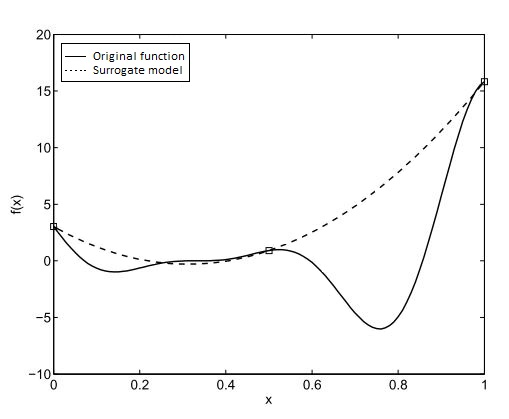
\includegraphics[width=8cm]{Images/Background/sbosexample.JPG}
		\caption[Example of a surrogate model]{Original function and corresponding surrogate model, created based on three initial solutions (squares). This image was retrieved from~\cite{Koziel2011}.}
		\label{fig:sbosexample}
	\end{figure}
	% End Figure -------------------------------------------------------
	
	Nowadays, the existing plethora of techniques applicable to the generation of surrogate models range from trust region methods to \ac{ML} techniques. These techniques can be used to create (1) local surrogates, i.e., models where the approximation to the objective function is built around a certain point, and (2) global surrogates, i.e, models where the approximation is generated from all the obtained points. Whilst the former relies on the construction of simple, partial models of the objective function, the latter relies on the creation of a full model. The creation of the full model, requires balancing the need for improving the accuracy of the model by exploring broader regions in the solution space, with the need for improving the value of the objective function by exploiting promising regions~\cite{Koziel2011}. This balance is determined by a strategy that selects the next promising solution to evaluate.
	
	Undoubtedly, the best feature of model-based algorithms is the reduction in the total optimization time. This is particularly relevant in the context of \ac{BPO}, where each simulation may take seconds, minutes, hours, days, or even weeks to complete. However, the lower availability and the lack of necessary technical knowledge to implement or incorporate these algorithms into optimization processes are still obstacles to a broader adoption of this approach. Notwithstanding the existence of different studies involving \ac{ML} techniques for the creation of full surrogate models~\cite{Koziel2011, Forrester2009SBO}, such as \acp{NN}, \acp{SVM}, \acp{RBF}, and \acp{RF}, among others, only a few have actually been applied in the context of architecture. This scenario is even more self-evident when we shift from the single- to multi-objective optimization context.
	
	% ----------- 
	\subsubsection{Comparison}
	\label{ssec:comparisondfo}
	
	This section compares the different classes of derivative-free optimization algorithms mentioned in this chapter. \Cref{table:compare-dfo-algos} presents a summarized view of the main properties of these classes and, in the following paragraphs we compare them regarding their applicability in architecture. 
	
	
	% Please add the following required packages to your document preamble:
	% \usepackage{multirow}
	% \usepackage{graphicx}
	\begin{table}[]
		\centering
		\resizebox{\textwidth}{!}{%
			\begin{tabular}{r|c|c|c|}
				\cline{2-4}
				& Direct search & Metaheuristic & Model-based \\ \hline
				\multicolumn{1}{|r|}{Main Mechanism / Strategy} & \begin{tabular}[c]{@{}c@{}}Sequential evaluation of \\ candidate designs\end{tabular} & \begin{tabular}[c]{@{}c@{}}Combine and randomly modify \\ previous known best designs\end{tabular} & \begin{tabular}[c]{@{}c@{}}Optimize a secondary model, \\ instead of the expensive one\end{tabular} \\ \hline
				\multicolumn{1}{|r|}{Deterministic} & Yes & No & Yes \\ \hline
				\multicolumn{1}{|r|}{Convergence guarantees} & Yes & No & Sometimes \\ \hline
				\multicolumn{1}{|r|}{Convergence rate (evals)} & Early (100-300) & Late (typically \textgreater{}1000) & Early (100-300) \\ \hline
				\multicolumn{1}{|r|}{Number of solutions} & 1 & More than 1 & 1 \\ \hline
				\multicolumn{1}{|r|}{Applicability to MOO} & Extremely rare & Very frequent & Unusual \\ \hline
				\multicolumn{1}{|r|}{Ease of use} & + & ++ & + \\ \hline
				\multicolumn{1}{|r|}{Ease of implementation} & + & +++ & + \\ \hline
				\multicolumn{1}{|r|}{Support in architecture} & + & +++ & + \\ \hline
				\multicolumn{1}{|r|}{\multirow{2}{*}{Main advantages}} & Deterministic & Applicable to any domain & Time complexity decrease \\
				\multicolumn{1}{|r|}{} & Convergence rate & Flexible & Convergence rate \\ \hline
				\multicolumn{1}{|r|}{\multirow{2}{*}{Main disadvantages}} & \multirow{2}{*}{\begin{tabular}[c]{@{}c@{}}Time complexity grows exponentially \\ with the number of parameters\end{tabular}} & Low convergence rate & \multirow{2}{*}{\begin{tabular}[c]{@{}c@{}}Time complexity grows exponentially \\ with the number of parameters\end{tabular}} \\
				\multicolumn{1}{|r|}{} &  & No convergence guarantees &  \\ \hline
			\end{tabular}%
		}
		\caption{Comparison between the derivative-free algorithms' classes.}
		\label{table:compare-dfo-algos}
	\end{table}
	
	
	The multidisciplinary aspect of building design raises distinct problems, ranging from well-behaved problems with simple, unimodal, convex functions to more ill-behaved problems with irregular, multimodal objective functions~\cite{Wortmann2017ADO}. In addition to problem's diversity, the time complexity associated to function evaluations also becomes an important factor to consider, when pondering each category's impact on \ac{BPO} problems.
	
	The problems' plethora within performance-based design is vast: a specific optimization algorithm may perform well for some problems and have a terrible performance in other problems~\cite{Wortmann2017GABESTCHOICE, Fang2017}. This idea resembles the ones captured in Wolpert's \acp{NFLT} for optimization, which state that any algorithm's worse performance over some classes of problems offsets its better performance in other classes. Because of the distinct nature of architectural design problems, the arguments applied in architecture are not necessarily applicable to the other fields, like science and engineering. 
	
	Inevitably, the same building design description might yield different problem descriptions according to the performance aspects being considered. Some algorithms might explore certain descriptions more effectively than others, e.g., because the objective functions describing the lighting and structural behavior of a certain design may have completely different properties. In an attempt to exploit this property, \ac{BPO} practitioners often dedicate a small amount of their total time budget to test various algorithms and different setup parameters, before finally settling for an optimization algorithm~\cite{Hamdy2016}.	
	
	Regarding the different algorithms' categories, it is interesting to see the metaheuristics' popularity among researchers and practitioners. The main reasons behind the idolization of the metaheuristics are their (1) inherent simplicity, (2) ease of implementation, and (3) wide applicability to different domains~\cite{Wortmann2017ADO}. Unfortunately, other categories do not benefit from such properties, which is a limitation towards their application in architectural domains. Moreover, the lack of easy-to-use tools involving algorithms from other categories are also limiting their application in architectural contexts. Firstly, the existing non-metaheuristic tools are usually available as programming libraries, instead of being integrated in architectural design workflows. As a result, to use the optimization algorithms, architects often need some programming knowledge to create the scripts to integrate the algorithms into the design workflow. However, since architects typically lack the required knowledge, they tend to struggle with the scripts' production and, eventually, opt for using friendlier metaheuristics ready-to-use tools. Given this facts, it is not surprising that most of the existing building design optimization literature ends up focusing on the application of algorithms from the metaheuristics category~\cite{Hamdy2016,Nguyen2014,Evins2013}. 
	
	However, in the light of the \acp{NFLT}, the need for more short-term efficient optimization approaches fostered the development of tools exposing algorithms with different properties. Particularly, plug-ins like Goat~\cite{GOAT} and Opossum~\cite{Wortmann2017Opossum} enable the usage of algorithms from both direct search and model-based classes. These tools expose optimization algorithms from the NLopt~\cite{NLOPT} and RBFOpt~\cite{RBFOPT} frameworks, respectively, providing friendly, ready-to-use interfaces within Grasshopper~\cite{GRASSHOPPER}, a visual programming environment that enables the parametric design and performance evaluation of building designs for different values of the parameters. For the past few years, few works have compared different algorithms using these tools with the ones available in other metaheuristics tools (e.g., Galapagos~\cite{GALAPAGOS}, Octopus\cite{OCTOPUS}, Optimo~\cite{OPTIMO}, Silvereye~\cite{Cichocka2017SILVEREYE}).
	
	Although the results may vary, in general, direct search and surrogate-based algorithms seem to be more effective than the metaheuristics ones in initial stages of the optimization process~\cite{Wortmann2017,Wortmann2016BBO,Wortmann2017GABESTCHOICE}. Even some metaheuristics algorithms can be very effective approaches for some optimization problems~\cite{Waibel2018}. One can explore these performance fluctuations to find the most effective optimization algorithm for a specific problem. This performance gain can be determining in the overall optimization time, especially when complex and time-consuming simulations are involved. Indeed, several authors ~\cite{Wortmann2016BBO,Hamdy2016} suggest that the selection of the optimization algorithm should be based on the results of several tests with different methods for a fixed number of evaluations or a fixed amount of time. 
	
	Optimization is a useful tool to address both single and multi-objective problems. In architecture, most optimization applications focus on single-objective problems and cover the three different derivative-free algorithms classes. However, the same does not happen with multi-objective problems, with only one of the classes being extensively applied to \ac{MOO} building design: the metaheuristics~\cite{Hamdy2016}. The main reason behind metaheuristics popularity is their broader adaptability to both varying degrees of complexity and to different problem domains~\cite{BlumRoli2003Metaheuristics}.
	
	Recent developments in multiple surrogate-assisted \acp{MOEA} in the fields of science and engineering~\cite{Zapotecas-Martinez2016,Hussein2016} made it possible to decrease the number of expensive evaluations in \ac{MOO} problems. Generally, these techniques combine metaheuristics methods, which find more than one solution within a single execution, with surrogate models, which are approximations of the original objective functions. Diaz-Manriquez et al.~\cite{Diaz-Manriquez2016} provide a comprehensive overview of surrogate-assisted techniques for \ac{MOO} from the engineering perspective. 
	
	The following sections focus on the current \ac{BPO} practices both for \ac{SOO} and \ac{MOO}, the currently available tools, and the advantages and disadvantages of each approach.
	
	
	
	\subsection{Performance Indicators}
	\label{ssec:performance}
	Despite the large interest in \ac{MOO}, the question of how to quantitatively compare the performance of different algorithms still remains unanswered. Firstly, in multi-objective problems, the number of objectives is greater than the number of objectives in single-objective problems: the former considers a collection of vectors representing the Pareto-optimal solutions, whereas the latter considers real numbers. Secondly, it is often the case that the application of exact methods to \ac{MOO} contexts is impracticable due to the complexity introduced by underlying applications (e.g., simulation tools, physical experiments). In these cases, the generation of the true Pareto-optimal set is often infeasible, requiring vast computational resources to be generated. Thirdly, despite the availability of alternatives to exact methods, such as metaheuristics algorithms (e.g., evolutionary algorithms, particle swarm), these are not guaranteed to identify optimal trade-offs, instead yielding good approximations~\cite{Zitzler2003Metrics}. Finally, we are interested in knowing which of the non-exact algorithms yields better approximations for a given problem, hence prompting the need for assessing the performance of \acp{MOOA}.
	
	The notion of performance includes not only the quality of the results, but also of the computational resources needed to generate such results. While the latter aspect is usually identical for both \ac{SOO} and \ac{MOO}, which either typically consider the number of expensive evaluations or the overall run-time on a particular computer, the quality aspect is considerably different. Because \acp{SOO} consider real-valued objective spaces, the quality is defined in terms of the objective function: the smaller (or larger) the value, the better the solution. However, \acp{MOO} consider vector-valued objective spaces, thus requiring another concepts like Pareto dominance. Unfortunately, when considering the Pareto dominance concept a few issues may arise, namely the possibility of two solutions being incomparable, i.e., when neither dominates the other, or having solutions in one set that either dominate or are incomparable to those in the other set of solutions and vice versa. 
	
	Literature review evidences the existing struggle to define the meaning of quality with respect to approximation of Pareto-optimal sets~\cite{Knowles2002Metrics,Riquelme2015}. However, the quality of Pareto sets is usually evaluated in terms of three aspects: (1) cardinality, meaning larger sets of solutions, (2) diversity, meaning that solutions should be as uniformly distributed as possible, so as to obtain a representative set of solutions covering to larger extents the different trade-offs, and (3) accuracy, meaning that solutions should be as close as possible to the true Pareto-optimal set or Pareto Front. 
	
	For the past decades, several indicators have been proposed to measure the quality of Pareto sets, ranging from unary quality measures, which assign each approximation set a number that reflects a certain quality aspect, to binary quality measures, which assign numbers to pairs of approximation sets, among others. This thesis considers a small but representative set of quantitative indicators to measure the quality of \acp{MOOA}' results with respect to the three aspects: cardinality, diversity, and accuracy. 
	
	Literature review reveals the existence of dozens of indicators that consider either one of the mentioned aspects or a combination of them. In the following definitions we use the term \textit{approximation set} to denote the Pareto Front returned by an optimization algorithm, and we use the term \textit{reference set} to denote the true Pareto Front or, whenever that is not possible, an estimate of the true Pareto front. 
	In this section, we list some of the most used indicators for assessing the performance of evolutionary \acp{MOO}~\cite{Riquelme2015}. 
	
	
	\subsubsection{Unary Indicators}
	% ---------------------------
	% Unary Indicators 
	% ---------------------------
	%% https://github.com/PastelBelem8/MscThesis/blob/metrics/src/indicators/MOOIndicators.jl
	% Cardinality 
	With regards to the cardinality aspect, there are essentially two indicators:
	\begin{itemize}
		\item \textbf{\ac{ONVG}} computes the number of non-dominated solutions in the approximation set ~\cite{Veldhuizen1999GD}.
		\item \textbf{\ac{ONVGR}} computes the ratio of non-dominated solutions in the approximation set with regards to a reference set~\cite{Veldhuizen1999GD}.
	\end{itemize}
	
	Cardinality indicators are based on the intuition that a good approximation set would have many optimal solutions. However, these indicators alone do not suffice to provide an accurate measure, as they privilege quantity over quality of solutions~\cite{Veldhuizen1999GD}, i.e., they often qualify approximation sets having dozens or hundreds of dominated solutions as being better than sets that provide fewer non-dominated solutions. This completely distorts the initial idea of finding the best Pareto front, i.e., set of non-dominated solutions.
	
	% || Diversity / Distribution ||
	To complement cardinality indicators, it is often advisable to consider the diversity aspect of approximation sets as well. A few well known diversity-based indicators are:
	\begin{itemize}
		\item  \textbf{Spacing} (or Set Spacing) computes the variance of the Manhattan distances between each non-dominated solution and its closest neighbor. It measures how well-spaced the solutions from the approximation set are. A value of zero represents equally spaced non-dominated solutions. 
		\item \textbf{Spread} (or $\Delta$) is similar to Spacing. However, it calculates the normalized variance and uses the Euclidean distance instead.
		\item \textbf{Maximum Spread} (or \textbf{$M_3^\ast$}) computes the Euclidean distance between the bounds of each objective dimension. It measures the extent of the objective space in each dimension by calculating the distance between the maximum and minimum of each objective. A greater value indicates larger coverage of the objective space.
		
		\item \textbf{Entropy} uses the Shannon's entropy concept to measure the uniformity of the approximation set distribution. This indicator makes the assumption that each solution provides some information about its vicinities, thus modeling each solution with Gaussian distributions. These distributions add up to form a density function capable of identifying peaks and valleys in the objective space, corresponding to dense and sparse zones, respectively. 
		
		\item \textbf{Diversity Metric} is similar to the Entropy indicator. However, it projects the solutions of both the approximation set and the reference set to an hyperplane which is subdivided uniformly. It assigns each interval two numbers: one number marking whether that interval contains at least one optimal solution in the reference set, and the second number marking whether the interval in addition to the optimal solution in the reference set, also contained at least one solution in the approximation set. Then, the diversity measure is the sum of the score of each interval, which are assigned using a sliding window technique (considering one interval and its immediate neighbors) based on the value of the marks\footnote{The scoring function considers the distribution of the marks in three consecutive grids. The function's proper definition can be found in \cite{Deb2002DM}.}. So, the diversity of the reference set considers the value of the first marks, whereas the diversity of the approximation set considers the values of the second marks. In the end, the diversity metric is given by the relative difference between the diversity of the approximation set and the diversity of the reference set. The best diversity possible is achieved if all intervals enclose at least one point\cite{Deb2002DM}.
		% Then, it computes the ratio between the number of intervals that have at least one non-dominated solution from both sets and the number of intervals that have at least one non-dominated solution of the reference set. Higher values of the diversity metric imply a better distribution and higher diversity of the approximation set when compared to the reference set itself. 
		
	\end{itemize}
	
	While these indicators are more robust, considering these indicators alone will not necessarily identify sets having Pareto optimal solutions, as they prioritize sets where solutions are spaced evenly apart or that cover broader regions of the objective space~\cite{Veldhuizen1999GD}. Moreover, because most of them assume that the Pareto front will be continuous, they may behave erroneously when facing problems with disconnected Pareto fronts. The diversity metric attempts to alleviate these limitations by comparing the non-dominated solutions of the approximation set with those of the reference set \cite{Deb2002DM}.
	
	% || Accuracy ||
	Previous metrics are not good indicators of how close the approximation sets really are to the reference set. To obtain a measure of the convergence of the results, one should consider accuracy indicators, such as:
	\begin{itemize}
		% ER
		\item \textbf{\ac{ER}} computes the proportion of false-positives in the approximation set, i.e., the ratio of optimal solutions in the approximation set that are not optimal in a given reference set~\cite{Veldhuizen1999GD}. Lower values of \ac{ER}, represent better approximation sets. 
		% MPFE
		\item \textbf{\ac{MPFE}} computes, for each solution in the approximation set, the minimum Euclidean distance to the closest solution in a given reference set, returning the maximum of those distances~\cite{Veldhuizen1999GD}. In other words, it returns the maximum error of the approximated Pareto Front. Lower values of \ac{MPFE} imply better approximation sets. 
		% Generational Distance
		\item \textbf{\ac{GD}} computes the average distance of an approximation set to a given reference set by computing the distance of the solutions in the approximation set to the nearest points in a given reference set averaged on the number of solutions in the approximation set~\cite{Veldhuizen1999GD}. A value of $0$ indicates that all the solutions in the approximation set are in the reference set. Different authors\cite{Zitzler2000m1m3} refer to this metric as \textbf{$M_1^\ast$}.
	\end{itemize}
	
	Accuracy indicators, like the previous indicators, can also produce misleading results and, therefore, should be considered together with other metrics. In general, all these three indicators have flaws, for instance, \ac{ER} focus on errors instead of focusing on the optimal solutions. As a result, it penalizes larger approximation sets that, despite having a more representative set of the real optimal solutions, have made more errors than other approximation sets with fewer solutions and, potentially, less errors. On the other hand, \ac{MPFE} focus on the maximum error of an optimal solution in the approximation set, when compared to the reference set. As a result, approximation sets, whose points are closer to the Pareto front but that have an outlier, will have higher values of \ac{MPFE} than other approximation sets, whose points are further away from the reference set but at a smaller distance than the outlier is from the reference set. At last, \ac{GD} has also been shown to behave erroneously, especially due to its dependency on the cardinality of the approximation set~\cite{Ishibuchi2005GDIGD}.
	
	The final set of indicators considers the accuracy and diversity aspects simultaneously:
	\begin{itemize}
		% Hypervolume
		\item \textbf{\ac{HV}} (or Lebesgue measure or S-metric) measures the size of the objective space covered by an approximation set, i.e., it measures the volume of the dominated space. It provides the unique and desirable properties of (i) Pareto \textit{compliance}, i.e., an approximation set which completely dominates another, will necessarily have a greater volume than the latter, and (ii) convergence guarantees, i.e., any approximation set that achieves the maximum possible volume is guaranteed to contain all Pareto-optimal solutions.
		% Inverted GD
		\item \textbf{\ac{IGD}} is the opposite of \ac{GD}, instead computing the average distance between a given reference set and the approximation set. \ac{IGD} computes the distances between each solution in the reference set and its closest solution in the approximation front, averaged over the size of the reference set. When the solutions in the reference set are well distributed, smaller values of \ac{IGD} suggest better and well-distributed approximation sets. Previous works have referred to this metric as \textbf{$D1_R$}~\cite{Ishibuchi2005GDIGD}\todo{Save REFs, a verdadeira ref está no Hansen1998}. 
	\end{itemize}
	
	Despite considering the diversity and accuracy aspects of Pareto fronts, \ac{IGD} is still Pareto non-compliant and has been shown to behave erroneously under certain conditions~\cite{Ishibuchi2005GDIGD}. Conversely, \ac{HV} is the only metric that exhibits the Pareto-compliance property. However, its usage is often impractical in problems, where the number of objectives is greater than ten, due to the its exponential grow with the number of objectives \cite{Ishibuchi2005GDIGD}.
	
	
	\subsubsection{Binary Indicators}
	In situations where the original Pareto-optimal set is not available, the binary indicators provide a way to compare approximation sets with respect to all the aspects. Among the most frequently used indicators, we emphasize:
	\begin{itemize}
		\item \textbf{Two set coverage} (or $C$) yields the number of solutions in one approximation set that are dominated by at least one of the solutions of the other approximation set. A value of $1$ suggests that the second approximation set is completely dominated by some solutions in the first one, whereas a value of $0$ represents the situation when none of the solutions of the second approximation set is covered by the first approximation set.
		
		\item \textbf{Epsilon Indicators} ($\epsilon$) that gives a factor by which an approximation set is worse than another considering all objectives, i.e., given two approximation sets $A$ and $B$, it computes the smallest amount $\epsilon$ by which $A$ must be translated, so that every solution in $B$ is dominated by at least one solution in $A$.
		
		\item \textbf{R-metrics} consider a family of indicators where the quality of each approximation set is defined according to a set of utility functions, and the larger the utility value of some set, the better the quality. R-metrics declare that the best approximation set will be the one that is better with regards to most utility functions:
		\begin{itemize}
			\item \textbf{$R1$} determines whether the an approximation set is better, equal, or worse than the other. 
			\item \textbf{$R2$} computes the expected mean difference in the utilities of both approximation sets.
			\item \textbf{$R3$} computes the expected mean relative difference in the utilities of both approximation sets.
		\end{itemize}
	\end{itemize}
	
	When comparing the usefulness of binary indicators, these usually aim at comparing different approximation sets and not necessarily the quality of the sets. This is the case of the two set coverage indicator, which allows to compare the existing Pareto-dominance relation between two sets, but does not allow to infer any other information (e.g., how worse one set is regarding the other). Moreover, this indicator becomes erroneous when the two sets are incomparable, i.e., neither dominates the other~\cite{Zitzler2003Metrics}. In contrast to the two set coverage indicator, the epsilon family indicators enable more informed comparison among two different approximation sets, as it provides a measure of the relative difference between the two sets. Finally, because the R-metrics incorporate utility functions, the user is able to introduce a preference over the objectives, thus influencing the optimality of each set. 

	
	
	
\section{Optimization in Architecture}
	
	
	\label{sec:plugins}
	
	For years, multiple derivative-free optimization libraries have been developed (e.g., NLopt, RBOpt, Platypus, DEAP, Pyomo, PISA, jMetal, MOEAFramework). However, in order to use them within architectural practices, architects had to code the integration scripts to connect the simulation models for different variations of the parametric models and the optimization libraries\cite{Attia2013}. Moreover, these frameworks often lacked post-processing and visual features, which antagonized the readability and comprehension of the results~\cite{Attia2013,Nguyen2014}.
	
	Several plug-ins have been developed in an attempt to reduce the limitations associated to the coupling of simulation tools and mathematical optimization frameworks, thus providing a seamless connection between the parametric models produced in computational design tools, like \ac{CAD} and \ac{BIM} tools, the simulation or analytical models, and the optimization frameworks. Given the visual nature of architects, these plug-ins provide friendly, ready-to-use optimization interfaces, which are usually coupled with a few post-processing and visual features to enhance the intelligibility of optimization results. 
	
	Currently, existing optimization plug-ins are implemented on top of the visual parametric tools: Grasshopper~\cite{GRASSHOPPER} and Dynamo~\cite{DYNAMOBIM}. In \Cref{fig:opt-plugins}, we represent the most relevant optimization plug-ins among \ac{BPO} practitioners: Galapagos, Goat, Octopus, Opossum, and Silvereye implemented on top of Grasshopper, and Optimo implemented on top of Dynamo. In the following sections we briefly discuss each plug-in.
	
	% Begin Optimization Plug-ins Figure -------------------------------------------------------
	\begin{figure}
		\centering
		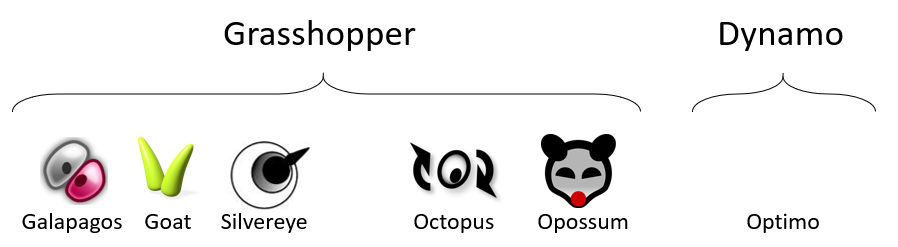
\includegraphics[width=\textwidth]{Images/Background/opt-plugins.PNG}
		\caption[Optimization Frameworks in the Architectural Practice]{Optimization frameworks currently used in architectural practices.}
		\label{fig:opt-plugins}
	\end{figure}
	% End Figure -------------------------------------------------------
	
	\subsection{Galapagos}
	\label{subsec:galapagos}
	% General description of Galapagos, intuition
	Galapagos~\cite{GALAPAGOS} is a generic plug-in, implemented on top of Grasshopper, designed to allow the application of metaheuristics algorithms by non-programmers to solve a wide variety of problems. 
	
	% Optimization Algorithms
	Particularly popular amongst architects~\cite{Wortmann2017ADO} for its \ac{GA}, Galapagos also provides other global metaheuristic solver, called simulated annealing (see \todo{referenciar secção dos algoritmos xD}). 
	
	% User Experience
	To use one of the solvers, architects must first define a script in using Grasshopper's components, such as sliders, values lists, area, distance, among others. This script should be organized in three distinct parts: (1) the Input, where they specify the design's parameters; (2) the Generation, where they create the design's algorithmic model that when instantiated with the parameters' values will generate the 3D model; and (3) the Analysis, where they define the analysis or objective function which they ought to optimize. 
	
	After creating the program script, the architect must drag the Galapagos' component to the script and connect it to the design parameters and to the objective function. Note, however, that Galapagos require the variables to be defined in terms of sliders components, interpreting their numerical range as the variables' lower and upper bounds, and the objective function to be output to a number component. The Galapagos' component refers to the variables as genome and to the objective function as fitness.
	
	Galapagos' \ac{GUI} is displayed upon double-clicking the Galapagos' component (see \Cref{fig:galapagosoptions}). The interface is simple, friendly, intuitive, and well-organized. Moreover, all options are filled by default, thus promoting a ready-to-use (or click-and-run) interaction, which makes it particularly easy to use by users with no experience or expertise in the field. Unfortunately, more experienced users might feel frustrated using this plug-in, as they are only able to modify a few parameters of the solver, thus lacking a finer control over the process. 
	
	In addition to not requiring any integration efforts or any programming-related knowledge to setup and use its capabilities, Galapagos also provides a visually rich experience, by providing different runtime graphical views of the optimization process. Galapagos supports different views depending on the optimization solver being used (see \Cref{fig:galapagosviewsa} and \Cref{fig:galapagosviewsb}):
	\begin{itemize}
		\item fitness graph that either represents the distribution of fitness values in the population discriminated by generations. Exhibited for both solvers;
		\item similarity representation graph that represents solutions that are genetically similar close to each other, and marks solutions that contribute to the creation of the next generation with black dots, whilst non-contributors are marked with a red cross. Exhibited for the \ac{GA} solver;
		\item vertical parallel coordinates graph, where each vertical line corresponds to a parameter, and solutions are represented as line segments connecting different parameters values. Exhibited for the \ac{GA} solver;
		\item ranked list of the best solutions found. Exhibited for both solvers;
		\item temperature graph, representing the temperature decrease rate of the simulated annealing process with each time step. Exhibited for the simulated annealing solver.
	\end{itemize}
	
	Overall, these views provide a visual feedback about the course of the optimization run and highlight the best solutions found up to that generation. In the end, the user is able to navigate through generations and re-instantiate these solutions in the corresponding \ac{CAD} tool, and, consequently to better understand the obtained results. Moreover, the ranked list of the results allow the user to select the one he appraises the most the amongst multiple optimal solutions found by the solver. Unfortunately, Galapagos lacks logging mechanisms which causes the information about the optimization enclosed within these views to be lost as soon as the \ac{GUI} is closed. 
	\begin{figure*}[htbp]
		\centering
		\subfigure[]{%
			\label{fig:galapagosoptions}%
			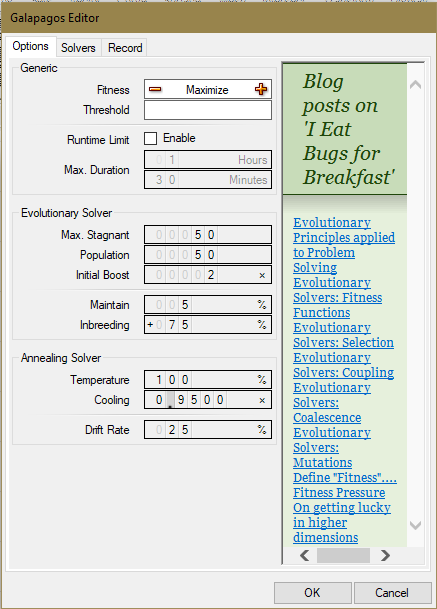
\includegraphics[width=0.30\textwidth]{Images/Background/Galapagos/Galapagos-algorithms-setup.PNG}}%
		\hfill
		\subfigure[]{%
			\label{fig:galapagosviewsa}%
			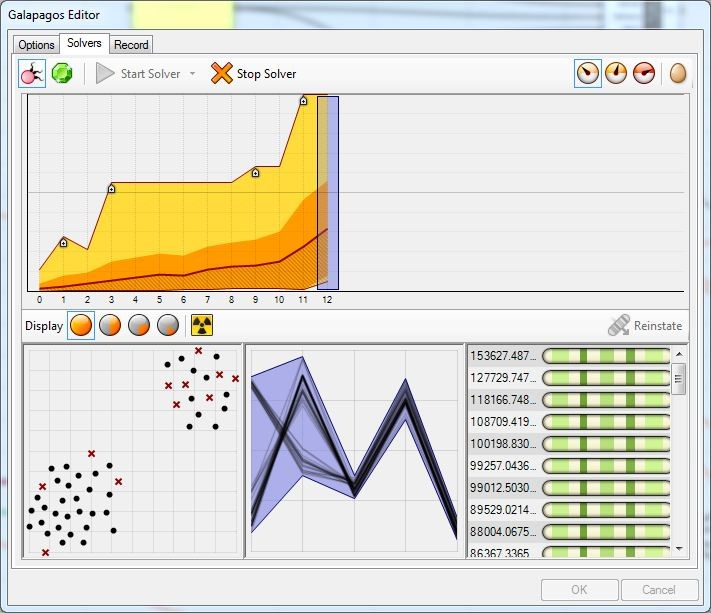
\includegraphics[width=0.345\textwidth]{Images/Background/Galapagos/galapagosvis.JPG}}%
		\hfill
		\subfigure[]{%
			\label{fig:galapagosviewsb}%
			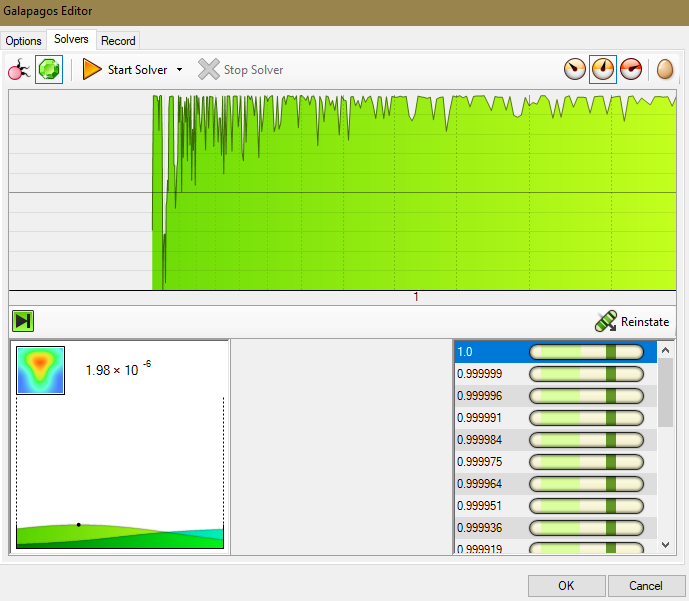
\includegraphics[width=0.345\textwidth]{Images/Background/Galapagos/galapagos-sa-results-2.PNG}}%
		
		\caption[Galapagos GUI]{ Three views of the Galapagos' \ac{GUI}: (a) Solvers configuration menu (b) Graphical views for the \ac{GA} solver (c) Graphical views for the simulated annealing solver}
		\label{fig:galapagos}
	\end{figure*}
	
	% ----------------- [GOAT] ------------------
	\subsection{Goat}
	% General description, intuition
	Goat \cite{GOAT} is a generic optimization plug-in, implemented on top of Grasshopper, designed to enable non-programmers to solve numerous problems.
	
	Unlike Galapagos, Goat interfaces the NLopt mathematical optimization library~\cite{NLOPT} to provide single-objective algorithms from all the derivative-free classes mentioned earlier (see \cref{sec:dfo}), including one global direct search (DIRECT), one local direct search (Subplex), one global metaheuristic (CRS2), and two local model-based algorithms (COBYLA and BOBYQA). 
	
	Goat is strongly influenced by Galapagos, also requiring a script in Grasshopper entailing the definition of the problem. In this script, the user drags the Goat's component to the script connecting it to the design parameters and the objective function, which, like Galapagos, must be sliders and number components, respectively (see \Cref{fig:goat}).
	
	Goat's \ac{GUI} is displayed after double-clicking the Goat's component (see \Cref{fig:goat}). This interface comprises a single menu, which is simple and straightforward to use. Like Galapagos, Goat is also distributed in a ready-to-use format with all the extra configuration parameters' values filled by default. As a result, non-programmers can easily explore this tool to address complex problems. Unfortunately, Goat provides no options for a more experienced user to configure the algorithms, except to configure the initial point of the search.
	
	Despite requiring no additional efforts to use Goat's optimization capabilities, the absence of visual and interactive mechanisms severely hinders the reputation of Goat. Firstly, it provides no visual feedback (e.g., solution lists, plots) about the course of the optimization run. Secondly, it also does not create log files to monitor the optimization process. Thirdly, the user is not able to interact with the optimization process. Finally, it returns a single optimal solution, whose values are represented in the sliders and number components. All these reasons contribute to a non-informed and non-traceable optimization process that inspires no confidence it the attained results. 
	
	% Begin Goat-Options Figure -------------------------------------------------------
	\begin{figure}
		\centering
		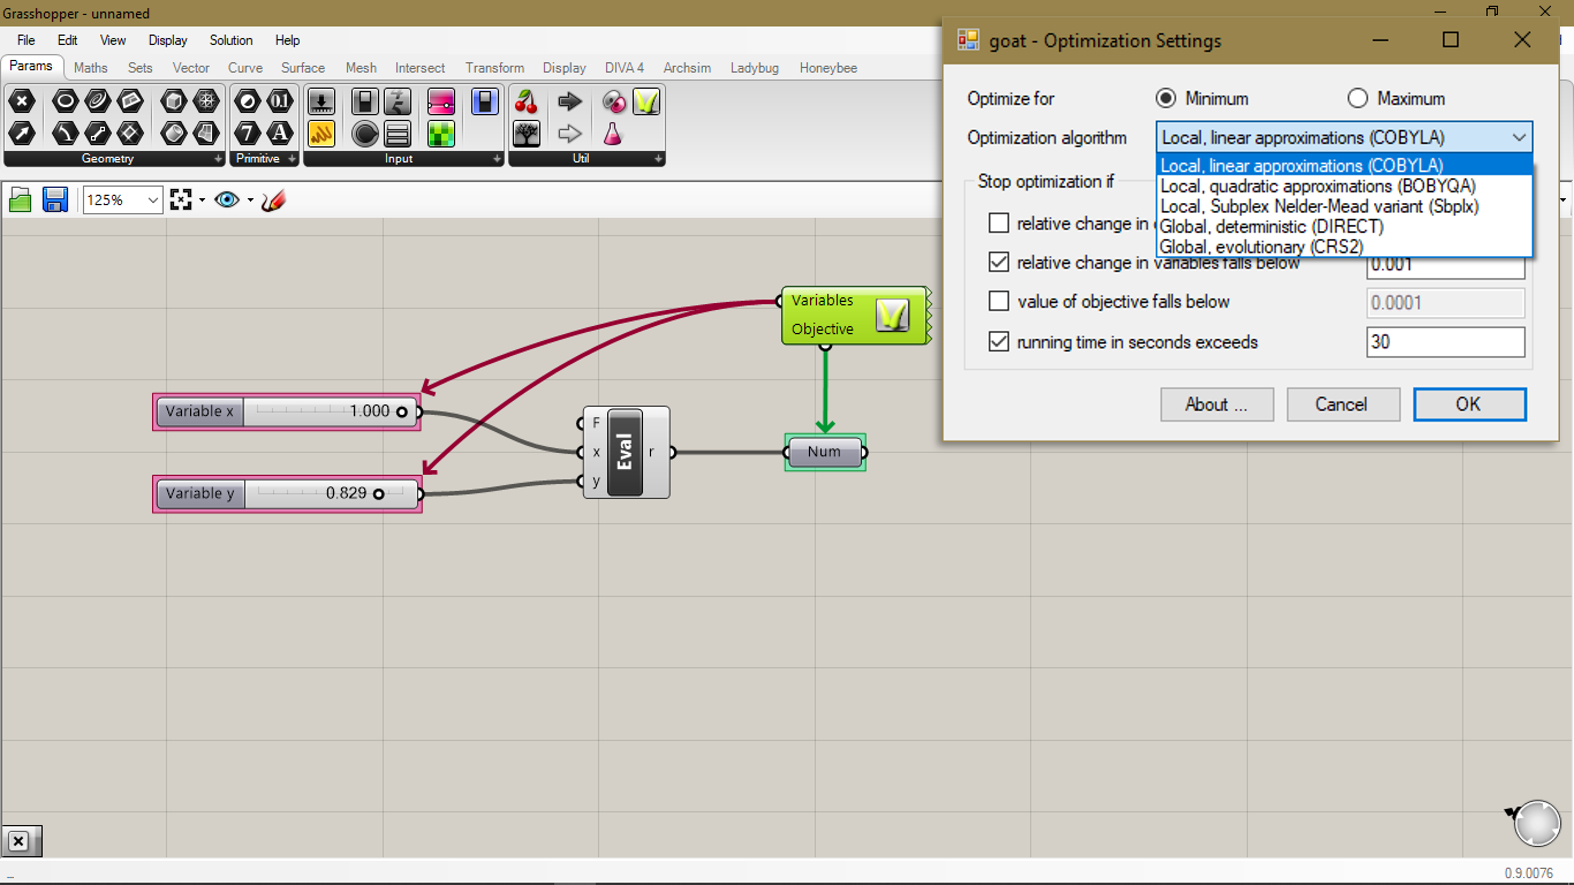
\includegraphics[width=1\textwidth]{Images/Background/Goat/general-view.png}
		\caption[Goat GUI]{Simple view of the Grasshopper's script with the problem definition and the Goat component. On the foreground, the \ac{GUI} exhibits the list of available algorithms within Goat}
		\label{fig:goat}
	\end{figure}
	% End Figure -------------------------------------------------------	
	
	
	% ----------------- [SILVEREYE] ------------------
	\subsection{Silvereye}
	Silvereye \cite{Cichocka2017SILVEREYE} is a generic optimization plug-in, implemented on top of Grasshopper, developed under the same design principles as Galapagos to enable non-experts to solve complex optimization problems. 
	
	Silvereye interfaces a C\# implementation of a global single-objective \ac{PSO} algorithm.
	
	Similarly to the previous tools, Silvereye also requires the definition of the problem in a Grasshopper script, and that the variables and the objective function value are represented by sliders and number components, respectively. Thus, it does not require any additional effort in order to be used.
	
	Likewise Galapagos, the user must double-click Silvereye's component in Grasshopper to visualize its \ac{GUI} (see \Cref{fig:silvereye}). Even though Besides being very simple and intuitive to use, Silvereye also allows less experienced users to start using the tool immediately by providing default values to the extra configuration parameters. As the users gain more experience, they might decide to change some configurations associated with the solver. One other difference to Galapagos is the ability to save the solver's configurations so that it can be used in subsequent runs.
	
	Regarding its visual capabilities, Silvereye is resemblant of Goat, providing no graphical views of the optimization run's state. However, Silvereye does present a list that is updated in real-time with the value of the best fitness value per iteration, which can be exported to a file and then used to create fitness graphs (see \Cref{fig:silvereye2}). Unfortunately, since this file merely contains the fitness values, the user is not able to trace them back to the values of the design parameters which originated them. Moreover, despite the existence of a functionality in the first menu (\Cref{fig:silvereye1}) to create a log file, this file only contains information about the temporal behavior of each evaluation. While this information is useful to monitor and identify irregularities during the optimization run, it does not provide enough information to traceback the error. 
	
	Overall, the lack of visual feedback in the form of graphs hinders the comprehension of and confidence on the results. The ranked list helps filling this gap, as long as there are multiple solutions and the user is able to visualize them in a \ac{CAD} tool.
	
	\begin{figure*}[htbp]
		\centering
		\subfigure[]{%
			\label{fig:silvereye1}%
			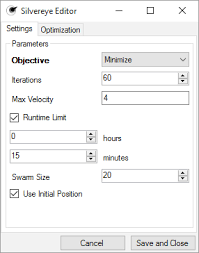
\includegraphics[width=0.40\textwidth]{Images/Background/Silvereye/silvereye.png}}%
		\hfill
		\subfigure[]{%
			\label{fig:silvereye2}%
			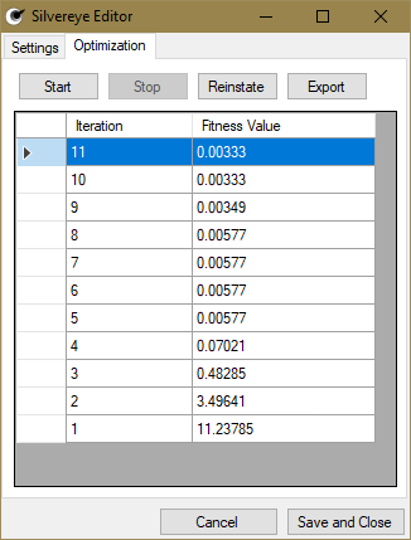
\includegraphics[width=0.40\textwidth]{Images/Background/Silvereye/silvereye2.png}}%
		
		\caption[Silvereye GUI]{Two views of Silvereye's \ac{GUI}: (a) Solvers configuration menu (b) Optimization control and results menu}
		\label{fig:silvereye}
	\end{figure*}
	
	%------------------ OPOSSUM ----------------------
	\subsection{Opossum}
	Opossum (OPtimizatiOn Systems with SUrrogate Models) \cite{Wortmann2017Opossum} is a generic plug-in, developed on top of Grasshopper, that explores Galapagos ideas to confer non-programmers an easy way to tackle a wide variety of problems.
	
	Opossum interfaces that the model-based RBFOpt library \cite{RBFOPT}, exposing two single-objective variants of the global \ac{RBF} algorithm. 
	
	In terms of usability, Opossum also resembles Galapagos, only requiring the definition of the problem in a Grasshopper script. To use the Opossum's solvers, the user must drag the Opossum's component to the Grasshopper script and connect it with the variables and the objective function components.
	
	Opossum's \ac{GUI} is simple, friendly, intuitive, and well-organized (see \Cref{fig:opossum}). In contrast to other plug-ins, Opossum presents different menus tailored for different levels of expertise. On the one hand, Opossum promotes a ready-to-use format, in order to ensure that less experienced users are able to use Opossum's capabilities. Therefore, Opossum provides two top-level configurations menus for which the values are already filled by default. On the other hand, Opossum provides more experienced users with the ability to create a finer configuration for the optimization solvers and, thus, achieve potentially more efficient optimization processes. 
	
	% Begin Opossum-Options Figure -------------------------------------------------------
	\begin{figure}
		\centering
		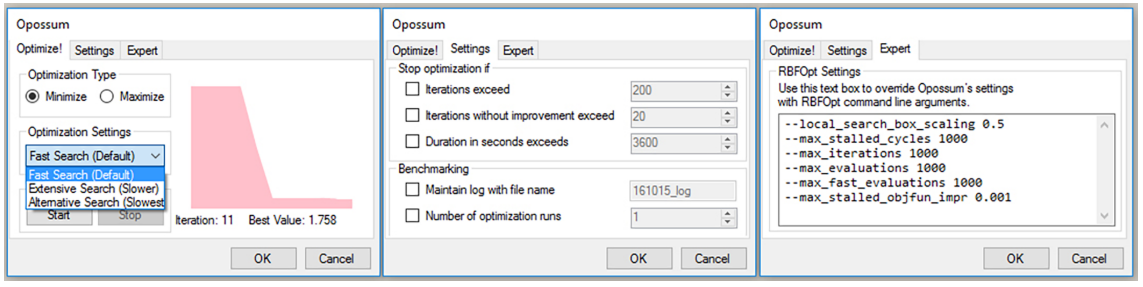
\includegraphics[width=1\textwidth]{Images/Background/Opossum/opossum_1.png}
		\caption[Opossum GUI]{The three views of Opossum's \ac{GUI}. Image retrieved from~\cite{Wortmann2017Opossum}}
		\label{fig:opossum}
	\end{figure}
	% End Figure -------------------------------------------------------
	
	The main deception of this plug-in lies in its visualization features. Although Opossum presents a fitness graph that is very useful for obtaining immediate feedback about the course of optimization, it does not provide an overview of the extent of the design space that is being explored, nor about the distribution of the designs that are being evaluated. Moreover, Opossum supports the creation of a log file that records all the solutions evaluated during the optimization run. Using other post-processing tools, the user can then either produce more insightful visualizations of the data, or re-use this information to create more accurate surrogate models, for example, for sensitivity analysis.
	
	One other disadvantage of this plug-in is the fact that the result of the optimization run is a single solution, instead of multiple ones. As a result, the intelligibility of results and the confidence on the process is greatly hindered, especially, due to its low visual support. 
	
	% ------------- [ Octopus ] -----------------
	\subsection{Octopus}
	
	Octopus \cite{OCTOPUS} is a generic plug-in, developed on top of Grasshopper, that allows non-programmers to address a wide variety of \ac{MOO} problems. 
	
	Octopus exposes two global metaheuristics algorithms, that explore evolutionary principles to search for Pareto-optimal solutions: \ac{SPEA2} and \ac{HypE} algorithms. These algorithms have been reported to yield promising results on numerous \ac{MOO} test problems~\cite{Zitzler2001SPEA2,Zitzler2011HypE}. 
	
	Even though Octopus was originally designed exclusively for optimization purposes, more recently, it focus has grown to include other \ac{ML} utilities, like supervised and clustering mechanisms. In fact, the first difference to the Galapagos-based plug-ins is related to this features' multiplicity, i.e., whereas previous Galapagos-based plug-ins focussed exclusively on optimization, Octopus covers multiple functionalities. This extra functionality is implemented as Grasshopper's components that are made available during Octopus' installation process under a tab that is created within Grasshopper (see \Cref{fig:octopus1}).
	
	The second difference affects the Grasshopper script. Like Galapagos, Octopus does require the definition of a Grasshopper script defining the variables and the objective functions. However, since Octopus focusses on \ac{MOO}, the user has to ensure that all the results of the objective functions are aggregated in single number component and then connected to the Octopus component. Additionally, because Octopus only performs minimizations, the problem definition must be modified to guarantee that all objectives are being minimized. One other important difference is that Octopus is able to tackle constrained problems. In this case, the hard constraints must be represented by a boolean component, and then connected to the Octopus component.
	
	After creating the Grasshopper script, Octopus \ac{GUI} can be accessed by double-clicking the Octopus component (see \Cref{fig:octopus2}). Despite its simplicity and friendliness, the \ac{GUI} is poorly organized and overloaded with information, hence making it difficult for a non-experienced user to locate any functionality in the interface. Although Octopus is distributed in a ready-to-use format, this plug-in exposes mechanisms to fine-tune a few parameters of the solvers. Even more surprising is the ability to change some of these parameters (e.g., elitism, mutation probability, crossover rate, mutation type) during runtime, thus increasing the user interactivity, and allowing the user to influence the optimization process.
	
	Octopus provides good support in terms of graphical feedback, providing three distinct views of the optimization problem (see views 1, 8, and 10 in \Cref{fig:octopus2}), namely:
	\begin{itemize}
		\item Solutions' Objective Space graph, which illustrates the distribution in the objective space of the solutions obtained during the optimization run. This graph also exhibits the approximated Pareto front that is currently known by the algorithm;
		\item Horizontal parallel coordinates graph, which serve the same purpose of the vertical parallel coordinates graph and that provide a view over the different design solutions that have been tested;
		\item Objective convergence graphs (one for each objective dimension), showing the upper- and lower-bounds of the Pareto front (dark gray) and the elite (light gray) of the number of history generations.
	\end{itemize} 
	
	Even though Octopus is capable of solving problems with up to five objective dimensions\footnote{Octopus uses the three spatial dimensions, color, and size to represent the five objective dimensions.}, the readability of these graphs becomes strongly damaged after the three dimensions. Besides the strong visual mechanisms, Octopus provides mechanisms to interact and instantiate each one of the solutions in the corresponding \ac{CAD} tool, which not only gives confidence to the user about the results, but also allows him to understand them better. Optionally, Octopus makes it possible to disable the real-time visualization of the optimization process with the aim of reducing the associated time penalizations.
	
	One other important feature of Octopus is the ability to create logs with the information about the evaluated solutions discriminated by generation. The only setback is that it does not allow to create a single file simultaneously containing the information about the design parameters and the objectives. 
	
	\begin{figure*}[htbp]
		\centering
		\subfigure[]{%
			\label{fig:octopus1}%
			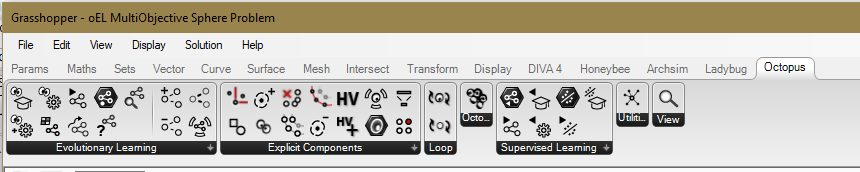
\includegraphics[width=1\textwidth]{Images/Background/Octopus/tab.PNG}}%
		\hfill
		\subfigure[]{%
			\label{fig:octopus2}%
			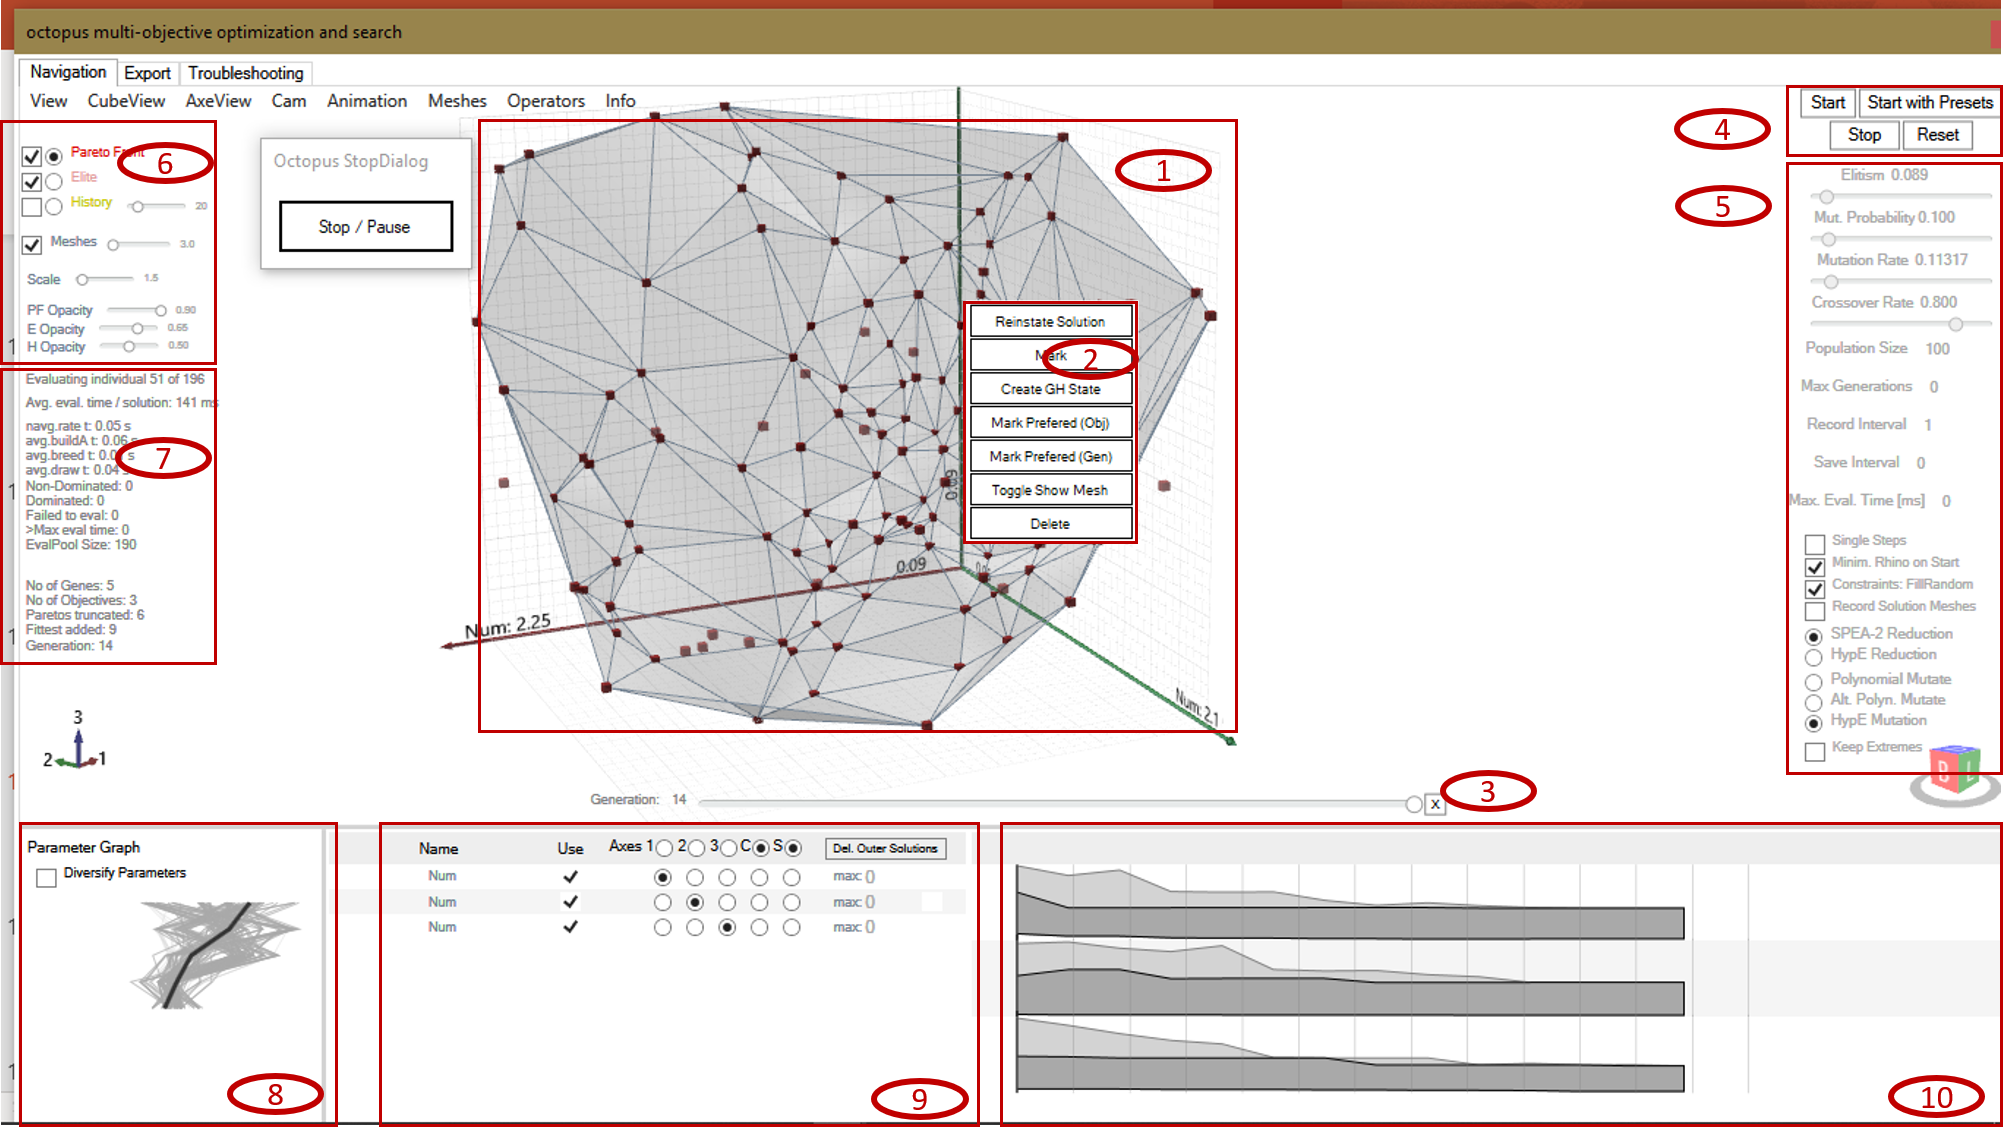
\includegraphics[width=1\textwidth]{Images/Background/Octopus/octopus-menu.png}}%
		\caption[Octopus GUI]{Octopus's \ac{GUI}: (a) Octopus menu in Grasshopper (b) Octopus optimization menu: (1) Solutions' Objective Space, (2) Solution's context menu, (3) Generation's history slider, (4) Process control options, (5) Algorithm Settings, (6) Display Settings, (7) Statistics, (8) Parallel Coordinates Graph, (9) List of Objectives (10) Convergence graphs per Objective}
		\label{fig:octopus}
		
	\end{figure*}
	
	
	% ------- ------- [OPTIMO] -------- ----------
	\subsection{Optimo}
	\label{subsec:Optimo}
	
	Optimo \cite{OPTIMO} is a generic plug-in, implemented on top of Dynamo, that allows non-programmers to address a wide variety of \ac{MOO} problems in the context of a \ac{BIM} tool. 
	
	Optimo interfaces the \ac{MOO} metaheuristics library, jMetal.NET and its current version merely supports the \ac{NSGA-II} algorithm\cite{Deb2002}.
	
	To use the solver, users must create the Dynamo script that encodes the problem definition, but also encode the optimization algorithm. To create the latter, Optimo provides four Dynamo nodes:
	\begin{itemize}
		\item Initial Solution list, which generates the initial set of random design configurations within a provided range and with the specified size of population;
		\item Assign Fitness Function Results, which evaluates and assigns the objective values to each configuration; 
		\item Generation Algorithm, which takes the parent population and generates the children population;
		\item Sorting, which uses the Pareto Front sorting to sort the solutions
	\end{itemize} 
	
	When compared to the previous plug-ins, Optimo demands larger initial investments for the production of the script. As a result, whereas less experienced users might find it more difficult to use, more experienced ones might adjust the algorithm to their needs, which directly results from the finer-grain control of Optimo. Moreover, instead of providing a default template, Optimo foster the constant arrangement of the algorithm's nodes everytime a new optimization process is to be applied, which can quickly become monotonous and tiresome. Moreover, Optimo does not have a explicit \ac{GUI} editor, instead being directly integrated in the Dynamo environment in the form of nodes.
	
	% Visual
	Regarding the visual mechanisms, it does not support feedback mechanisms during the optimization run, only presenting a small side-by-side view of the initial design variation and the optimal designs, thus allowing the user to visualize and compare the results of the optimization process. Finally, we were not able to conclude whether Optimo enabled the creation of log files or not. 
	
	% Comparison
	\subsection{Comparison}
	
	\Cref{table:pluginscompare} shows a comparison between the optimization plug-ins analysed in this chapter at the light of four aspects: (1) the optimization algorithms; (2) the interaction and visualization mechanisms; (3) the comprehension of results; and (4) the user experience.
	
	Taking into account the first aspect, we can observe that most optimization tools focus on single-objective and global optimization. Regarding the diversity of the algorithms most plug-ins provide either one or two options with the exception of Goat which provides five different algorithms from different derivative-free classes. Apart from Goat and Opossum, all other plug-ins support exclusively metaheuristics algorithms.
	
	When considering the interactivity and visualization mechanisms of the explored tools, all plug-ins but Goat yield multiple solutions and allow the user to interact with it and re-instantiate these solutions directly in the corresponding \ac{CAD} or \ac{BIM} tool. Surprisingly, only Galapagos, Opossum, and Octopus present graphical feedback mechanisms. Particularly, Galapagos and Octopus provide not only mechanisms about the state of the optimization (e.g., parameters values being explored, current fitness values), but also provide an overall ranking of the best solutions. On the other hand, none of the plug-ins except for Octopus enable the user to influence and interact with the optimization process during its execution. Even the interactions supported by Octopus are very limited consisting of the modification in runtime of the values of the elitism, mutation, and crossover operators. Regarding the traceability feature (e.g. creation of logs, solutions' lists), it is poorly supported. While Goat has no traceability, both Galapagos and Silvereye provide a ``semi-traceable'' list with the fitness values of the best attained solutions. At last, both Opossum and Octopus support, in a way, the creation of logs describing the state of the whole optimization process, i.e., information about the evaluated design variations with their parameters and corresponding objectives values.
	
	Regarding the third aspect, there are no mechanism explicitly designed to enhance the comprehension of the optimization results in any of the analysed tools. However, the existence of visualization mechanisms like Galapagos and Octopus, do enable a better understanding of the the results. This understanding can be further improved by enabling the direct materialization of such solutions in the corresponding 3D model, so that the user may draw conclusions by comparing different solutions. Despite the absence of visual mechanisms in Octopus, Octopus exhibits the best solutions next to the initial solution, thus allowing the user to compare them and better understand them.
	
	Finally, regarding the user experience, all plug-ins are straightforward to use, except for Octopus and Optimo. Both plug-ins require the user to elaborate the program in order to be run, but they differ, however the former requires a single component to be added, whereas the latter requires the definition of the solver using the provided nodes.
	
	\todo{Tratar disto. Resize box está a escalar a fonte também}
	\begin{table}[]
		\centering
		\resizebox{\textwidth}{!}{%
			\begin{tabular}{cl|cccccc|}
				\cline{3-8}
				\multicolumn{1}{l}{} &  & \multicolumn{1}{c|}{Galapagos} & \multicolumn{1}{c|}{Goat} & \multicolumn{1}{c|}{Silvereye} & \multicolumn{1}{c|}{Opossum} & \multicolumn{1}{c|}{Octopus} & Optimo \\ \hline
				\multicolumn{1}{|c|}{\multirow{4}{*}{Optimization Algorithms}} & Objectives & S & S & S & S & M & M \\
				\multicolumn{1}{|c|}{} & Search & G & GL & G & G & G & G \\
				\multicolumn{1}{|c|}{} & Classes & Meta & ALL & Meta & Model & Meta & Meta \\
				\multicolumn{1}{|c|}{} & Algorithms & 2 & 5 & 1 & 2 & 2 & 1 \\ \hline
				\multicolumn{1}{|c|}{\multirow{4}{*}{Interactivity and Visualization}} & Results & M & S & M & S & M & M \\
				\multicolumn{1}{|c|}{} & Graphical Feedback & +++ & - & - & + & +++ & - \\
				\multicolumn{1}{|c|}{} & Real-time Interactivity & - & - & - & - & + & - \\
				\multicolumn{1}{|c|}{} & Traceability (e.g., logs) & + & - & + & ++ & ++ & ? \\ \hline
				\multicolumn{1}{|c}{Intelligibility of Results} &  & + & - & - & - & + & + \\ \hline
				\multicolumn{1}{|c|}{\multirow{3}{*}{GUI Experience}} & Ease of Use & +++ & +++ & +++ & +++ & ++ & - \\ \cline{2-2}
				\multicolumn{1}{|c|}{} & Intuitive/Organized & ++ & +++ & +++ & +++ & + & + \\ \cline{2-2}
				\multicolumn{1}{|c|}{} & Flexible (e.g., fine-tune) & + & - & + & +++ & ++ & ++ \\ \hline
			\end{tabular}%
		}
		\caption[Comparison between the analysed optimization plug-ins]{A comparison between the analysed optimization plug-ins. S - single, M - multi, G - Global, L - Local.}
		\label{table:pluginscompare}
	\end{table}
	% Falar de cada 
	
	
	
	
	
	
	
	
	
	
	
	
	
	
	
	
	

% #############################################################################
\section{Problems to Address}
\label{sec:problemsaddress}

Despite the existence of both optimization  (e.g., DEAP, MOEAFramework, NLopt, RBFOpt), and visualization (e.g. Matplotlib, Plotly, Seaborn) libraries, architects often lack the programming skills necessary to integrate them into an optimization process. 

% Scalablity, portability, code legibility
Several optimization tools integrated in the architectural design workflow have been proposed throughout the years (see \cref{sec:plugins}). In general, these tools are easy to learn and use, which also results from the fact that they make use of visual programming languages. However, the visual programming paradigm often leads to scalability and program's legibility issues, hence impacting the way users interact with these optimization tools. 

On the other hand, the textual paradigm does not face from these scalability issues. Currently existing \ac{AD} tools (e.g., Khepri) do not support optimization, but already provide the primitive mechanisms to create automated optimization processes. Moreover, \ac{AD} tools usually offer portability of their programs, thus allowing architects to visualize and analyze their models in different 3D modeling and analysis tools, without the need to change the program.

% Single-Objective
In contrast to the multi-objective view of most \ac{BPO} problems, where architects aim to optimize multiple aspects simultaneously, most of these tools focus on \ac{SOO}. The usage of these tools often requires the simplification of the corresponding \ac{MOO} problem either by relaxing the objectives or by assigning preferences to each objective (see \cref{subsec:preferencesarticulation}).

% Global optimization
Most tools only provide global optimization support. While global optimization algorithms are good for obtaining close to optimal solutions, these often fail to provide more exact solutions. Particularly, not only are local optimization algorithms able to find more exact solutions but they also do so faster, especially if provided with useful initial information, such as the starting point.

% Unconstrained Optimization
% Moreover, the analyzed plug-ins do not provide explicit support for hard constraints on the variables, other than the lower and upper bounds on the values of variables. While that suffices for some cases, it is not enough for many other cases in building design, where variables must relate to other according some specific relation (e.g., size of a window must be smaller than the size of the enclosing wall). 

% Metaheuristic Optimization
Also, in terms of the optimization algorithms, most tools adopt metaheuristics algorithms. While these algorithms are flexible and applicable to nearly almost domain, they lack convergence guarantees, often requiring hundreds or thousands of evaluations to reach good results. Especially for simulation-based problems with time-consuming evaluations, these numbers are a main obstacle for the application of optimization. The situation becomes even more complicated  in the \ac{MOO} context, as the number of evaluations raises exponentially with the number of objectives. This problem can be partially reduced by using model-based algorithms, where a secondary and faster model is used for evaluation.

% Visualization
Regarding the visualization, most plug-ins do not provide enough visual information about the optimization state and the results themselves. Inclusively, most of them generate poorly formatted files with insufficient information, thus impeding to trace back the process and even hindering the comprehension of the results (e.g., associate the design parameters' configurations with the corresponding performance values). Even if users use external tools to produce visualization mechanisms based on the information exported from the optimization plug-ins, these are often only available in the end of the optimization run. As a result, the computer or the system crashes during the optimization run (e.g., energy failure), no log file will be produced and all the information collected by the plug-in will be lost. 

At last, most tools do not offer the possibility for interacting with them, nor do they provide means to pause and resume optimization runs. This is an inconvenience because it impedes users to add the knowledge they have learned, i.e., during the optimization run users would ideally extract information from good visualization mechanisms, that they could add to the process to make it more efficient.

Taking all the \textit{pros} and \textit{cons} of the analyzed tools into consideration, our solution enables the user to use a derivative-free optimization tool to address not only \ac{SOO} but also \ac{MOO} problems. The solution also provides integrated visualization mechanisms that aim to complement and enrich the information extracted during an optimization run. 

Additionally, our solution is flexible enough to allow the user to select between a set of algorithms with different properties \cite{Wolpert1997NFLT}, including algorithms that handle time-consuming evaluations. By providing algorithms from different classes, our solution potentiates the efficiency of optimization processes. In order to help in the choice of the algorithms, our solution also adds support to easily run benchmarks with multiple algorithms, providing a quantitative measure of their performance. 

Our solution also values the traceability of results especially for enhancing user comprehension. To improve existing mechanisms, our solution produces files involving all the necessary information about the configurations (e.g., algorithm parameters) and the solutions evaluated during the optimization process. Using these files, we are able not only to input them to other post-processing tools (e.g., visualization, statistics), but also to hot start and pause/resume optimization processes.

At the light of the architectural practice, our solution makes use of the textual programming paradigm and, consequently, has a special affinity with textual \ac{AD} tools (e.g., Khepri). As a result, when coupled with these \ac{AD} tools, our solution also benefits from their portability and scalability properties. We aim at reducing the abnormal time-complexity of \ac{BPO} by providing model-based algorithms. 

Finally, we consider the complexity of our solution. Unlike the analyzed tools, our solution does not benefit from the visual paradigm, which means that it should be simple to use and intuitive, even for non-programmers. As a result, we hide the complexity of the integration of optimization libraries under an abstraction layer, providing a clean and succinct set of primitives. These primitives draw inspiration from simple optimization mathematical models and should be rather intuitive and easy to use. 

In the next chapter, we describe the architecture of our solution and explain how each component achieves the features highlighted in this section.


% #############################################################################
\section{TROUBLEMAKERS}
- GALAPAGOS
% Available Algorithms
Galapagos provides two metaheuristics algorithms, namely, the genetic algorithm, inspired by biological evolution processes, and the simulated annealing, motivated by the metallurgical process of annealing \cite{Brownlee2011}. Although both algorithms are the basis for a large variety of extensions and/or specializations, supporting different heuristics, we will not provide a full description of such extensions, instead referring the interested reader to proper literature throughout this section. 

% Algorithms description
As evolutionary algorithms, genetic algorithms explore Darwinian natural selection concepts, such as heredity, reproduction, and natural selection, and genetics concepts and mechanisms, including genes, chromosomes, recombination, crossover, and mutation, in order to search for better solutions in the solution space. More concretely, genetic algorithms generate an initial random set of solutions, called population, which is then iteratively evolved, creating new generations. The evolution process is comprised of four main phases: (1) adaptability, where individuals of the population are assigned a suitability or fitness value; (2) selection, where pairs of individuals are selected for reproduction, based on a probabilistic function which is proportional to each individual's fitness value; (3) crossover, where the genotypes of the selected individuals are recombined to produce new individuals; and (4) mutation, where new individuals are subjected to random copying errors with a certain probability. While earlier generations are usually diverse, final generations are often very similar to the fittest individuals, i.e., we observe an intensification of the traits of the most suitable individuals, thus emulating the mechanism of natural selection, described by Darwin \cite{Brownlee2011}. Besides genetic algorithms \cite{Golberg1989,Holland1992}, evolutionary algorithms encompass other algorithms such as Genetic Programming~\cite{Koza1992}, Evolution Strategies \cite{Schwefel1981}, Differential Evolution \cite{Storn1997}, among others. 

Besides genetic algorithms, Galapagos also provides a metaheuristics global optimization physical algorithm, the simulated annealing. Resemblant of hill climbing algorithms, where new candidate solutions are randomly sampled, this algorithm iteratively re-samples the solution space aiming at finding an optimal solution. During the search, the algorithm is propitious to accept the re-sampled solutions with lower performance, according to a probabilistic function that becomes more discerning of the quality of the samples over the execution of the algorithm, thus resembling the natural annealing process~\cite{Brownlee2011}. 


- GOAT ------------------------------------------------------------------------------
% Available Algorithms
One of the key differences between Goat and Galapagos is the number and diversity of the algorithms available. Whilst Galapagos supports two global metaheuristics algorithms, Goat supports five distinct algorithms: one metaheuristic, two direct-search, and two model-based algorithms, called CRS2, DIRECT, SUBPLEX, COBYLA, and BOBYQA, respectively. Due to space constraints, a full description of these algorithms will not be provided, instead we refer the interested reader to the relevant literature.  

% METAHEURISTICS METHODS ------------------------------------
% CRS2
The CRS2 algorithm is a variant of the \ac{CRS} algorithm for global optimization~\cite{Price1983}. A \ac{CRS} algorithm is a population-based random search algorithm that creates an initial set of points, the population, which are then randomly evolved by means of heuristic rules. In the original \ac{CRS} algorithms, heuristic rules modify a point at a time, replacing the worst point with a better one (called trial point), using a technique resemblant of the \ac{NMS} algorithm \cite{Nelder1964}. Similarly to \ac{NMS}, \ac{CRS} algorithms use a simplex, i.e., a generalized triangle in N dimensions, to envelope a region described by a random subset of points in the population. The worst point of the population is replaced with the reflection of the worst point in the simplex~\cite{Kaelo2006CRS2}. The CRS2 variant differs from the original in that it assumes that the worst population point will always be a part of the simplex. The actual version that is made available by Goat is a modified version of the CRS2 algorithm that introduces a local mutation component in an attempt to overcome situations where heuristic rules constantly fail to find a trial points that actually improve the worst point. Fundamentally, this local mutation generates a second trial point that results from the exploitation of the region around the best point in the population~\cite{Kaelo2006CRS2}.  \todo{Vantagens e desvantagens ? Lack sound convergence properties, robustness and performance are highly problem dependent ~ler Kaelo}

% DIRECT-SEARCH METHODS ------------------------------------
% DIRECT
The second algorithm is a global deterministic direct search algorithm that relies on the division of rectangles, as explained in ~\cite{Jones1993DIRECT}. DIRECT, the DIviding RECTangles algorithm, recursively subdivides the design space into smaller multidimensional hyper-rectangles, estimating the quality value of each rectangle. DIRECT uses these values to focus the search on more promising regions of the design space and to further subdivide those in smaller hyper-rectangles. 
% SUBPLEX	
The SUBPLEX algorithm is an unconstrained local optimization algorithm~\cite{Rowan1990}. As a generalization of the \ac{NMS} algorithm, SUBPLEX subdivides the design space in low-dimensional subspaces and then applies the \ac{NMS} algorithm to a set of these subspaces, in order to seek for a better solution. In contrast to \ac{NMS}, which has difficulties in high-dimensional problems, SUBPLEX reduces the limitations through the decomposition of the problem in low-dimensional subspaces which are more efficiently optimized by \ac{NMS}.

% MODEL-BASED METHODS ------------------------------------
Besides metaheuristics and direct-search algorithms, Goat also provides two local model-based implementations, namely the COBYLA (or Constrained Optimization BY Linear Approximation) algorithm~\cite{Powell1994COBYLA}, and the BOBYQA (or Bound Optimization BY Quadratic Approximation) algorithm~\cite{Powell2009BOBYQA}, that rely on the construction of simple, partial models of the objective function~\cite{Koziel2011}. The former uses the concept of simplex to iteratively generate linear approximations of the objective function, whereas the latter generates quadratic approximations instead. 

One of the main advantages of Goat is the algorithms' diversity. By providing algorithms with different characteristics and strategies, architects can test the suitability of each algorithm to their problem and, thus, select the most effective. The right choice may result in large optimization gains, especially when complex and time-consuming simulations are necessary~\cite{Wortmann2016BBO}. For this reason, and due to the uniqueness of each \ac{BPO}, several authors suggest that the selection of the optimization algorithm should be based on the results of several tests with different algorithms for a fixed number of evaluations or a fixed amount of time~\cite{Hamdy2016,Wortmann2016BBO}. Moreover, the distinction between global and optimal algorithms is also critical when striving for accurate and precise optimal solutions. Most global optimization algorithms invest most of their effort searching for the truly optimal solution across large regions of the search space and rarely focusing on promising regions. Consequently, they might return a not so precise global optimum. To overcome this lack of precision and accuracy, one should apply a local optimization algorithm and provide the globally imprecise optimum as input.

- Silvereye ------------------------------------------------------------------------------
% Algorithm
The \ac{PSO} algorithm is a global metaheuristic algorithm inspired by biological systems, such as the collective behavior of flocking birds and schooling fish, which interact and learn from one another to solve problems~\cite{Brownlee2011}. In \ac{PSO}, the intelligence is decentralized, self-organized, and distributed throughout the participating particles, also known as swarm. These particles maintain information about their velocity, their current and personal best positions, and also the global best position known to the swarm. At each time step, the position and velocity of each particle are updated according to the best swarm or close neighbor position~\cite{Brownlee2011}.

- Opossum ------------------------------------------------------------------------------
Opossum is a model-based optimization tool for Grasshopper that uses the \ac{RBF} machine learning technique to create global approximations of the objective function~\cite{Forrester2009SBO}. These approximations are simply the weighted sum of other, simpler, real-valued functions, the radial functions. These functions are defined on the Euclidean space $\mathbb{R}^n$ and their value depends on the distance to a center $c$, so that $\phi(x, c) = \phi(\left\lVert x-c \right\rVert)$. In a \acp{RBF} technique, the weights are estimated based on the interpolation of data. A comprehensive detailed explanation of the \ac{RBF}'s estimation process is provided in~\cite{Forrester2009SBO}. 

Since its invention, multiple implementations of \ac{RBF} have been proposed. RBFOpt implements two well-known versions, namely, the Gutmann's~\cite{Gutmann2001} and the Regis and Shoemaker's~\cite{Regis2007}, commonly known as MSRSM. These techniques differ in the search strategy for the next candidate solution to be evaluated using the original objective function. The former uses the solution, which is likely to yield the largest improvement in the surrogate's accuracy, whereas the latter tries to balance the surrogate's accuracy amelioration with the exploitation of promising solutions, using other search strategies, such as genetic algorithms, sampling algorithms, or other mathematical solvers~\cite{Wortmann2017Opossum}. Moreover, RBFOpt provides five different types of radial basis function: linear, multi-quadratic, cubic, thin plate spline, and automatic selection, which are also provided in the Opossum interface.

- Octopus ------------------------------------------------------------------------------
%Octopus enables the simultaneous search for more than one objective, producing a set of possible optimal solutions that ideally represent the real trade-offs between each objective. In order to search for the Pareto-optimal solutions, Octopus provides two main evolutionary algorithms: \ac{SPEA2} and \ac{HypE}. On the one hand, due to their population-based nature, evolutionary algorithms are able to approximate the Pareto Front in a single run~\cite{Zhou2011}. On the other hand, these algorithms have been reported to yield promising results on numerous test problems~\cite{Zitzler2001SPEA2,Zitzler2011HypE}.

Similarly to evolutionary algorithms, \acp{MOEA} adopt the evolutionary principles discussed in \cref{subsec:galapagos} but, generally, have an additional archive to store the non-dominated solutions found~\cite{Zitzler2001SPEA2}. The archive technique is incorporated to prevent losing current non-dominated solutions due to random mutations or recombinations. Most \acp{MOEA} differ in the selection and reproduction operators used to iteratively evolve populations. These differences are usually related to the very own goals of approximating the Pareto Front: (1) maximize the accuracy of the approximation (by minimizing the distance to the optimal front) and (2) maximize the diversity of the solutions within the front. While the first goal is related to the search strategy and how to assign fitness values in such a way that the individuals selected for offspring production will be closer to the Pareto-optimal front, the second goal is related to the time and storage constrains of the evolution process and which individuals to keep in each generation \cite{Zitzler2001SPEA2}. Although a thorough description of different \acp{MOEA} and their mechanisms is not herein presented, we refer the interested reader to \cite{Zhou2011}. 

Most modern \acp{MOEA} realize the accuracy and diversity ideas through some implementation of the following mechanisms~\cite{Zitzler2001SPEA2}:	
\begin{itemize}
	\item Selection (or environmental selection): Besides the population, most \acp{MOEA} maintain an archive with the non-dominated front among all the solutions that were evaluated. The archive preserves individuals during several generations, only removing them if (1) a new solution is found to dominate them, or (2) if the archive size is exceeded and they happen to be in crowded regions of the front.
	
	\item Reproduction (or mating selection): At each generation, individuals are evaluated in two stages. The first stage compares them regarding the relation of Pareto dominance, using this information to define a ranking among these individuals. The second stage refines these rankings through the incorporation of density information, i.e., if the individuals lie in crowded regions.
\end{itemize}

These mechanisms can be completely indifferent from one another, e.g., the first one applying a Pareto-based criteria and the second one applying weighting approach. However, many \acp{MOEA} implement both concepts similarly. In the particular case of \ac{SPEA2}, the algorithm explores two independent sets of individuals: the population and the archive. In this algorithm, the archive size is fixed and, therefore, whenever the number of non-dominated individuals is less than its size, some dominated individuals are added to the archive. At each iteration, the algorithm computes each individual's fitness value (a \textit{strength} value, defined as terms of the number of solutions it dominates, the \textit{raw fitness} value, defined in terms of the strength of its dominators, and a density estimate, defined as the inverse of the distance to the $k^{th}$ to the nearest neighbor) and copies the non-dominated individuals from the population to the archive, removing any individual that is dominated, whose objective values are duplicated, or that, when the size of the updated archive is exceeded, lies in crowded regions of the non-dominated front. After filling the archive, pairs of individuals are chosen from the archive to reproduce and produce the offspring through recombination and mutation operators that will make the population of the next generation~\cite{Zitzler2001SPEA2}.

Unfortunately, algorithms incorporating the Pareto dominance relation and diversity measures appear to have difficulties in optimization scenarios with more than two objectives, which spurred the development of algorithms using other quality measures, including quality indicators. To overcome the objective limitation and provide the user with the flexibility to use a more efficient algorithm, Octopus provides the option to use \ac{HypE}, an algorithm that explores the \ac{HV} indicator to rank individuals. Particularly, to minimize time penalties associated with the computation of the \ac{HV}, in scenarios with more than three objectives, \ac{HypE} uses Monte Carlo simulations to estimate the \ac{HV} value of each individual~\cite{Zitzler2011HypE}. 

% 	https://pdfs.semanticscholar.org/dbc6/99826d7d28a75a304e715b796c8d2ee3dc90.pdf


% Optimo ------------------------------------------------------------------------------
% Algoritmo
As a \ac{MOEA}, \ac{NSGA-II} attempts to achieve an approximation to the Pareto front that is both accurate and diverse. In this particular algorithm, both the selection and reproduction mechanisms rely on the same basis criteria: Pareto dominance relations and a crowding measure. To define the order among the individuals, the pool of individuals is split into different Pareto fronts and ranked accordingly, i.e., the first non-dominated front is assigned the highest rank, the second front is assigned the second highest rank, and so on. Each individual in each rank is ordered according to a crowding measure, represented in terms of the sum of distances to the two closest individuals along each objective. The archive and the generation's population are combined, deleting the worst 50\%. Afterwards, binary tournaments are carried out on the remaining individuals (the archive members) in order to generate the next offspring population.

% If Printing on DOUBLE SIDED pages, the second page should be white.
% Otherwise, comment the following command:
\cleardoublepage
%
%Chapter 3
% #############################################################################
% This is Chapter 3
% !TEX root = ../main.tex
% #############################################################################
% Change the Name of the Chapter i the following line
\fancychapter{Architecture of the Optimization Framework}
% The following line allows to ref this chapter
\label{chap:architecture}

This dissertation focus on the study of optimization algorithms that are able to handle more efficiently a set of problems involving time-consuming functions. Apart from the theoretical study and literature review, this dissertation proposes a framework to enable the application of different types of optimization algorithms, both for \ac{SOO} and \ac{MOO} problems. The concretization of such framework requires: (1) the definition of an abstraction layer, that enables the modeling of optimization problems, (2) a wide variety of optimization algorithms to address different optimization problems, (3) a set of performance indicators to provide the user with a measure of the algorithms' quality when testing multiple algorithms, and (4) visual representations of the obtained results to provide more comprehensive feedback over the optimization results. ~\Cref{fig:solution} shows the  solution's different components and its external connections.


\begin{figure}[htbp]
	\centering
	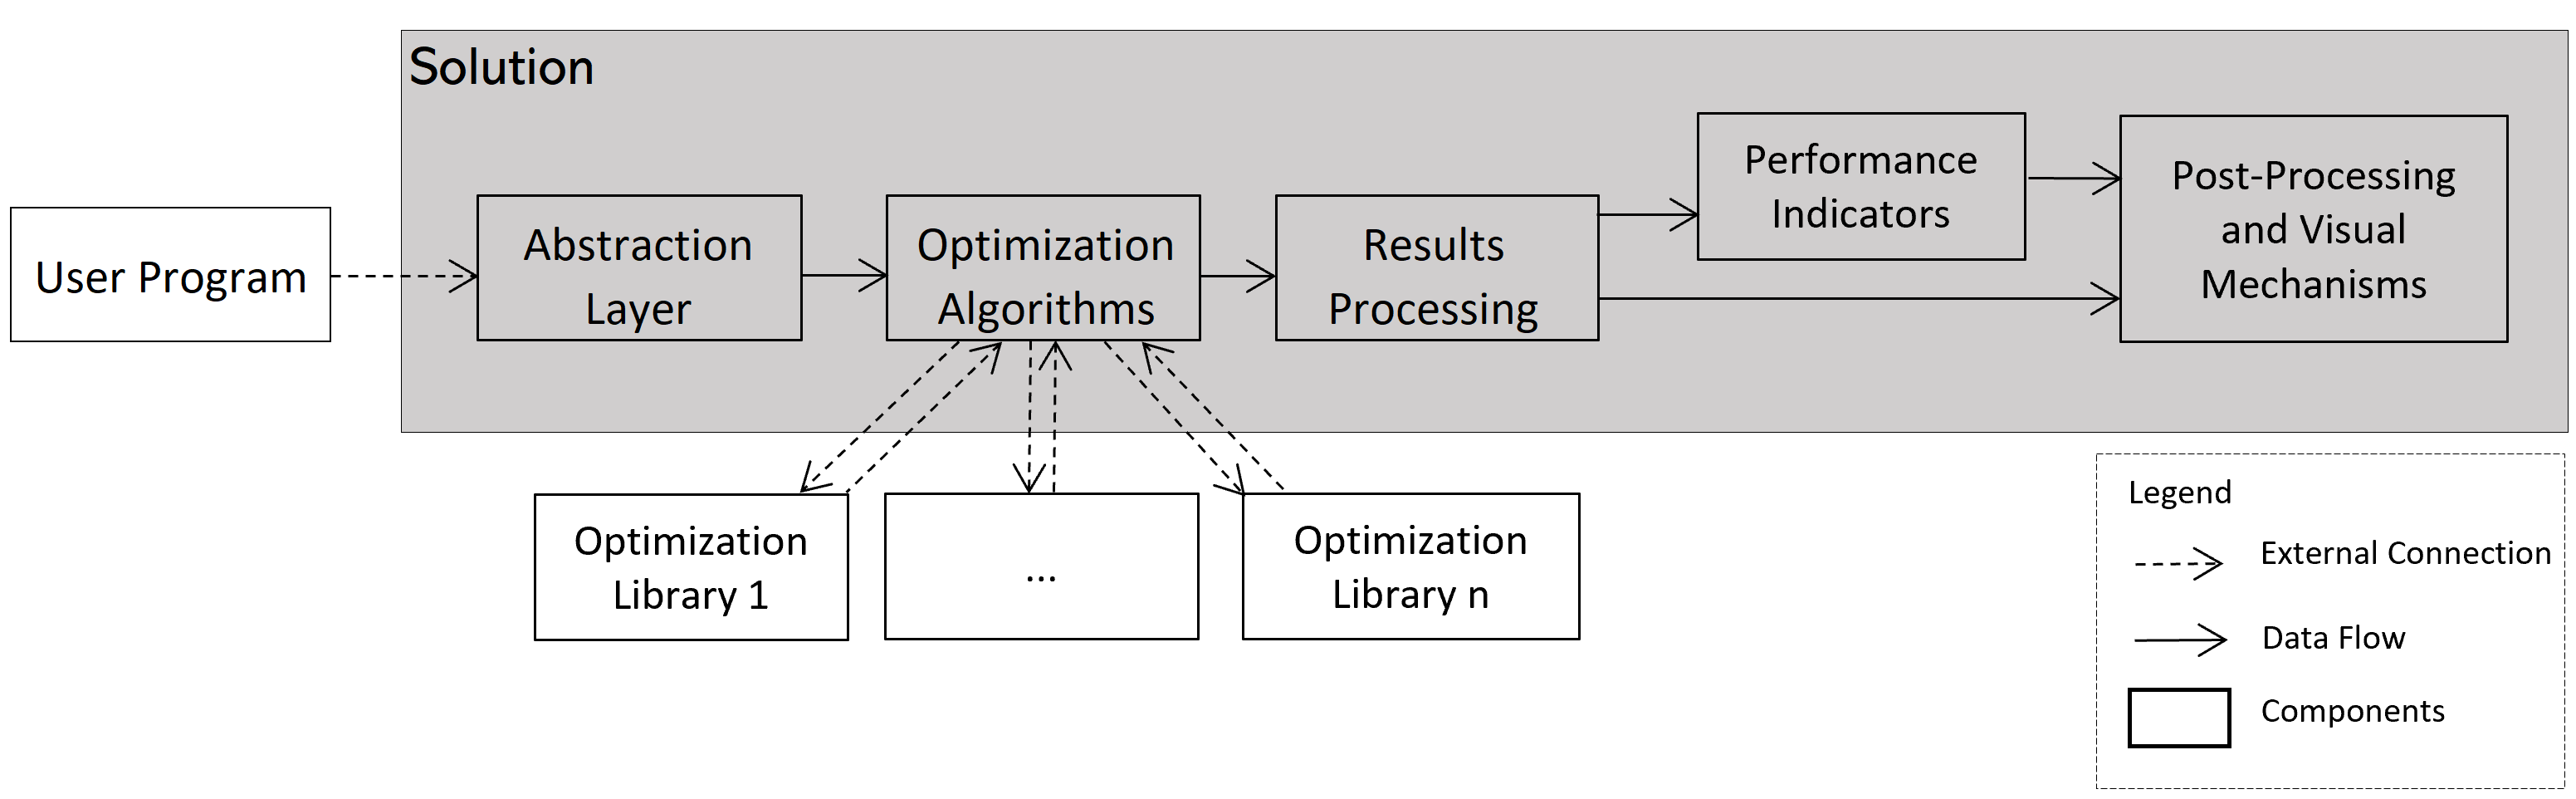
\includegraphics[width=\textwidth]{./Images/Solution/solution_architecture_2.PNG}
	\caption{Architecture of the solution.}
	\label{fig:solution}
\end{figure}

With the aforementioned framework, users are able to address optimization problems involving time-intensive functions, for which the objective functions' analytical forms are unavailable. In order to verify its executability and suitability for conducting multiple optimization processes, we developed a prototype of such framework. This chapter describes the main components of the developed framework and also the main requisites that led to their implementation. 


\section{Programming Language}
\todo{Não dar tanto detalhe? Parecer que é uma escolha secundária.}
One of the first concerns when developing the framework was regarding which programming language to use. The currently implemented framework uses two programming languages, which were chosen based on the available optimization libraries, the domain of the solution, and the performance of each programming language.
 
On the one hand, several languages already provide well-known optimization libraries, which have been tested, and independently validated. As a result, instead of attempting to implement the optimization algorithms again, we sought for programming languages which provided an easy access to these implementations. On the other hand, because we are dealing with optimization algorithms that involve numerical computations, we aimed at languages which provided fast numeric computation without the need to dive into lower level languages, such as C or Fortran. Finally, the performance of the programming language and also the mechanisms provided by the language to make code development more efficient (e.g., avoiding boilerplate code).

The first programming language is Julia\footnote{https://julialang.org}, a recent programming language that has been shown to be very promising in the numerical optimization domain, and that provides mechanisms to speed code development (e.g., functional programming paradigm, macros). Despite having a smaller library's repository than, for instance, Python\footnote{https://www.python.org/}, Julia has grown to implement some of Python's optimization libraries (e.g., Scikit-learn, NLopt), and, therefore, also provides some of the same functionalities of Python.   

Unfortunately, Julia is a juvenile language and, whilst some of these libraries can effectively become more efficient (e.g., Scikit-learn), other libraries present some limitations regarding the supported functionalities. For instance, in terms of data processing and visualization, Python presents a more stable  and better documented set of libraries (e.g., Pandas, Seaborn, Matplotlib, Plotly). For all these reasons, in order to facilitate the processing and visualization of the optimization results, we adopted Python as the second programming language.

% Furthermore, the data transfer between Julia and Python is easily achieved by using the mechanisms provided by Julia (e.g., macros) and a wrapper library, PyCall. \todo{Nao sei muito bem como melhorar isto.. Mas o vocabulario está um bocado simplorio...}

One aspect to take into consideration is that, albeit being implemented in Julia and Python, our solution could have been implemented in other programming languages such as Java or C++, which also provide several optimization and data processing libraries. In this dissertation and as it will be explained in ~\Cref{chap:implement,chap:evaluation}, we had the extra motivation that the case studies were already developed in Julia. Thus, by creating an abstraction layer in Julia, we were able to easily integrate optimization processes with an existing algorithmic tool in architecture, and to easily test the effectiveness and quality of the proposed solution within the architectural context. 

\section{Abstraction Layer}
The abstraction layer is designed to abstract the user from the logic of other external optimization tools. By providing a uniform \ac{API}, i.e., a set of primitives and procedures, this abstraction layer eliminates the appearent chasm between different optimization tools and facilitates the use of algorithms from different optimization libraries, incurring no additional efforts for the user, i.e., the user is not required to make any further modifications to the program, e.g., changing the program structure, changing the primitive operations, in order to test different optimization algorithms. 

By adopting one of the currently available domain-specific modeling languages for optimization (e.g., JuMP, PyOMO, MultiJuMP, PISA, AMPL), not only would users have access to a well-tested and more stable \acp{API}, but they would also have out-of-the-box access to a wide variety of optimization solvers capable of handling various problems. 

Notwithstanding their benefits, the abstraction layer provided in this dissertation does not make use of these modeling languages due to (1) their lack of support for both \ac{SOO} and \ac{MOO} problems, (2) complexity of syntax rules and need for deep understanding of the language to use it, and (3) lack of solvers or mechanisms that enable the execution of optimization solvers capable of efficiently addressing optimization problems involving costly simulation-based evaluation functions. As a result, to explore one of these modeling languages would require not only additional developments to create the mechanisms to support both \ac{SOO} and \ac{MOO} problems, but also to create a new solver capable of addressing the specific type of problems that this dissertation set out to address. 

Nevertheless, influenced by existing optimization modeling languages, the abstraction layer's operations remove the complexity associated to most of modeling languages and allow to incrementally combine them in order to model more complex optimization problems. Moreover, the abstraction layer is designed to enable the execution of any of the optimization approaches discussed in~\Cref{sec:optimizationproblems}, ranging from \ac{SOO} to \ac{MOO} approaches, passing through the design of experiments approach.

\todo{ADD COLOR}
\begin{lstlisting}[caption={Simple example of the framework's API.},label=juliaCode]	
using MScThesis

# Define variables
vars = [RealVariable(-10, 10)]

# Define objectives
f1(x) = x[1]^2
f2(x) = (x[1] - 2)^2
objs = [Objective(f1, :MIN), Objective(f2, :MIN)]

# Create the optimization problem
model = Model(vars, objs)

# Optimize it!
solve(NSGAII, model, max_evals=100)
\end{lstlisting}

As described in \Cref{chap:back}, the definition of an optimization process is composed of two parts: the modeling of the optimization problem and the optimization algorithm. This \ac{API} provides not only primitives to define variables, objective functions, and, when necessary, constraints, but also empowers users with the ability to use and fine-tune the parameters of each optimization algorithm, i.e., parameters that control the detail of the search process. The entire \ac{API} is intuitive and simple to use by less experienced users, but flexible to be extended and improved by programmers, which may decide to add more algorithms or integrate other optimization libraries.  \Cref{juliaCode} illustrates how to use the framework's \ac{API} to model a bi-objective unconstrained optimization problem. To this end, in order to solve the problem, the user needs to: (1) create the model of the problem (\textit{line 12}), which requires the definition of the variables (\textit{line 4}) and the objective functions (\textit{lines 7 to 9}); (2) to specify the optimization algorithm (\textit{line 12}), which in this case is the \ac{NSGA-II}; and (3) the maximum number of costly evaluations during the optimization search.


\section{Optimization Algorithms}
\label{sec:optalgos}

Optimization algorithms represents a crucial part in an optimization process and, consequently, in the developed solution. In order to study different optimization algorithms and to test their suitability for specific optimization problems~\cite{Wolpert1997NFLT}, a large set of distinct and representative optimization algorithms should be provided. In addition to diversity, our solution also provides the users with the flexibility to configure the different parameters associated to the optimization algorithms, commonly known as hyperparameters. By fine-tuning the values of these hyperparameters for a specific problem, the performance of optimization optimization can be drastically improved. 

One other important requisite, considered by the developed solution, is that at least a subset of the provided algorithms must be tailored to address optimization problems that incorporate time-consuming evaluation functions and for which information is difficult to obtain. To address this requisite, we reviewed the most reputed \ac{SOO} and \ac{MOO} open-source derivative-free optimization libraries. After a thorough analysis of different optimization libraries, the final solution exposes a total of 36 algorithms from 4 different libraries, listed in \Cref{table:algorithms}. 


\begin{table}[]
	\centering
	\begin{tabular}{cccll}
		\rowcolor[HTML]{EFEFEF} 
		\textbf{Class} & \textbf{Objectives} & \textbf{Global} & \textbf{Algorithm} & \textbf{Library} \\ \hline
		& Both & G & K-factorial & None \\
		& Both & G & Latin Hypercube & None \\
		& Both & G & Random & None \\
		\multirow{-4}{*}{Sampling} & Both & G & Stratified Random & None \\ \hline
		& S & G & CRS2 & NLopt \\
		& M & G & CMA-ES & Platypus \\
		& S & G & ESCH & NLopt \\
		& M & G & ES & Platypus \\
		& M & G & $\epsilon$-MOEA & Platypus \\
		& S & G & GA & Platypus \\
		& M & G & GDE3 & Platypus \\
		& M & G & IBEA & Platypus \\
		& S & G & ISRES & NLopt \\
		& M & G & MOEAD/D & Platypus \\
		& M & G & NSGA-II & Platypus \\
		& M & G & NSGA-III & Platypus \\
		& M & G & PAES & Platypus \\
		& M & G & PESA2 & Platypus \\
		& M & G & SPEA2 & Platypus \\
		& M & G & OMOPSO & Platypus \\
		\multirow{-17}{*}{Metaheuristic} & M & G & SMPSO & Platypus \\ \hline
		& S & G & DIRECT & NLopt \\
		& S & G & DIRECT-L & NLopt \\
		& S & L & NMS & NLopt \\
		& S & L & PRAXIS & NLopt \\
		\multirow{-5}{*}{Direct search} & S & L & Subplex & NLopt \\ \hline
		& S & L & BOBYQA & NLopt \\
		& S & L & COBYLA & NLopt \\
		& Both & G & Decision Tree & Scikit-learn \\
		& Both & G & GP & Scikit-learn \\
		& Both & G & Linear & Scikit-learn \\
		& Both & G & MLP & Scikit-learn \\
		& Both & G & Random Forest & Scikit-learn \\
		& Both & G & RBF-Cubic & pySOT \\
		& Both & G & RBF-Linear & pySOT \\
		\multirow{-10}{*}{Model-based} & S & G & SVR & Scikit-learn
	\end{tabular}
	\caption[Solution's list of supported algorithms]{List of the algorithms exposed by the currently implemented solution, discriminated by class, number of objectives, aim of the search, and the optimization library implementing it. Note: L - Local, G - Global, M - Multi, S - Single.}
	\label{table:algorithms}
\end{table}
To implement sampling algorithms, the framework makes use of Julia's arrays and random primitives, requiring no additional libraries to be implemented. Secondly, by integrating the NLopt~\cite{NLOPT} library within our framework\footnote{A special thanks to Guilherme Ilunga who contributed to this integration.}, we were able to expose 10 \ac{SOO} algorithms and, thus, to test algorithms from the three derivative-free optimization classes. Moreover, this library has already been used in Goat~\cite{GOAT}, an architectural design optimization tool, which has been applied in some architectural studies as well~\cite{Wortmann2017ADO}. Thirdly, the Platypus library was chosen from a set of \ac{MOO} libraries, that included Platypus, jMetal, MOEAFramework, Paradiseo, and PaGMO. The Platypus library was the final choice due to the variety and quality of the \ac{MOO} algorithms provided, the ease of integration with the Julia programming language, and the cleanness and readibility of its \ac{API}. Finally, the last integrated library was Python's scikit-learn, which provides the basis algorithms for constructing more complex model-based algorithms, both for \ac{SOO} and \ac{MOO} problems.

When providing a framework that interfaces multiple libraries, it is important that the \ac{API} remains simple, abstracting the user from the different logic associated with the integrated libraries. To this end, the developed framework exposes a single and unified \ac{API}, enabling users to easily apply algorithms from different libraries and requiring no additional efforts or modifications (e.g., change the invocation method, change the name of parameters) from the user. Additionally, in order to extend the currently framework with other optimization algorithms, the programmer is only required to implement a connector between the proposed \ac{API} and the optimization library's \ac{API}.

 
\section{Performance Indicators}

One of the goals of this thesis is to compare different optimization algorithms and assess the influence of their inherent mechanisms and assumptions in the overall performance of optimization processes. To this end, it is necessary to have a simple way of verifying the quality of these algorithms. 

To this end, the solution enriches the abstraction layer previously discussed with a set of performance indicators. While for comparing \ac{SOO} algorithms, these indicators usually resume to discovering both the value of the best found solution and the number of evaluations (or time) required to reach that value, for comparing \ac{MOO} algorithms this solution implements a subset of the indicators discussed in \Cref{ssec:performance}, namely, the unary indicators: \ac{ONVG}, \ac{ONVGR}, spacing, spread, maximum spread, \ac{ER}, \ac{GD}, \ac{HV}, and \ac{IGD}, and the binary indicators: R-metrics, $\epsilon$ indicators, and the two set coverage.

Notwithstanding the utility of quantitatively qualifying the performance of different algorithms, this information can be difficult to interpret by less experienced users. To enhance interpretability, the proposed solution introduces post-processing and visualization functionalities discussed in the next section. Particularly, in the architectural context, where architects often lack knowledge about optimization, visual and post-processing mechanisms become very important to promote a better comprehension and enable the making of more informed decisions. 

\section{Visual and Post-Processing Mechanisms}

%  Why do we want visual and post-processing mechanisms ?  Why is it important? 
Often disregarded by any optimization tools, the possibility to choose a solution among the best found solutions is highly advantageous. Firstly, it allows users to examine the best found solutions and to choose the one that better fits their needs. As an example, consider the optimization of a specific aspect of a building design. It is often the case, that the solution returned by the optimization algorithm is not the preferred solution, either because of more subjective opinions or, even, because the best solution for that aspect might negatively impact other aspects which are not being considered (e.g., increasing the daylight illuminance often has repercussions on the thermal conditions and on the energy consumptions of a building). Secondly, it enables the examination of different equally optimal solutions and the selection of the solution that better fits the user's needs. This is particularly useful when handling with multi-modal problems, for which there can be distinct solutions that yield the same optimal value. Unfortunately, many optimization tools obliterate most of these solutions, only providing the user with one solution. Finally, sometimes close to optimal solutions suits better the user intentions. By providing both optimal and close to optimal solutions, users would be empowered with a better understanding of optimization results and possibly to make more informed decisions. 

% How does our solution improves this?
The framework developed in this dissertation uses Python's data processing and visualization libraries, including, Pandas, Scikit-learn, Matplotlib, Seaborn, and Plotly to produce post-processing and visualization scripts that can be interpreted and manipulated by users to enrich the information obtained from optimization processes. 

By providing a simple way of visualizing different views of results (e.g., statistics, distribution, correlations, parallel coordinate graphs, pareto front, convergence graphs) and for post-processing them (e.g., outliers removal, interpolation of results), users are able to better understand the optimization process. 

Moreover, unlike many currently existing optimization tools, our solution provides out-of-the-box mechanisms to provide traceability and predictability about optimization processes. The solution preserves information regarding the configurations (e.g., model of the optimization problem, algorithm parameters), the optimization results, which are updated during the course of the optimization process. 

To further take advantage of these files, our solution exposes a set of primitives in the abstraction layer that allows the reuse of optimization results' files by providing them as input data for other optimization algorithms. This feature can be particularly relevant when testing different optimization algorithms in problems involving time-consuming simulation-based evaluation functions, as it allows to save computational time.

% Using these files, we are able not only to input them to other post-processing tools (e.g., visualization, statistics), but also to hot start and pause/resume optimization processes.

% Limitations
Although the implemented prototype does not provide real-time data information about the currrent state of the optimization process, our framework can be easily extended to include those features, since it rests on a fortified mechanism of real-time logging, that preserves both the configurations and the results involved in the optimization process. Additionally, because these files are updated in real-time, these mechanisms can be updated if rerun again by the user. With this ability users are able to examine in real-time the solutions that have already been evaluated by the optimization process and decide if the any of the found solutions already fulfills their intentions, or if they should wait for the optimization process to finish. 


\todo{bonecos, gráficos...}


% If Printing on DOUBLE SIDED pages, the second page should be white.
% Otherwise, comment the following command:
\cleardoublepage
%
%Chapter 4
% #############################################################################
% This is Chapter 4
% !TEX root = ../main.tex
% #############################################################################
% Change the Name of the Chapter i the following line
\fancychapter{Algorithmic Optimization in Architecture}
%\cleardoublepage
% The following line allows to ref this chapter
\label{chap:implement}
In the previous chapter, we discussed the architecture of the proposed solution, a general-purpose optimization framework that is applicable to a wide variety of optimization problems. 

From the beginning, we set out to address optimization problems involving simulation-based objective functions that are remarkably expensive. Therefore, during the development of the proposed framework, we focused on providing algorithms to more efficiently handle problems exhibiting these properties. Note, however, that the framework can be easily extended to include other algorithms (e.g., derivative-based), as it has been previously discussed in \cref{sec:optalgos}. 

Motivated by the large impact of the building sector in the world's sustainability and economy, this dissertation aims at applying the proposed framework to address \ac{BPO} problems, thus attempting to reduce buildings' costs and ecological footprint. Despite the existence of multiple optimization tools in architecture, as discussed in \cref{sec:optimizationtools}, these are often limited and do not provide adequate algorithms, nor mechanisms to enable the efficient optimization of such time-consuming problems.

In this chapter, we describe how the general-purpose framework proposed in this dissertation can be applied to address architectural design optimization. 

\section{Algorithmic Optimization}
In \cref{ssec:ad,ssec:aa}, we discussed how the architectural design paradigm has incrementally grown to develop the mechanisms to quickly (1) update a design, (2) generate the corresponding analytical model, and (3) automatically evaluate the design in an analytical tool.% and collect its results. 

These mechanisms laid down the foundations for automated optimization processes. By extending the Algorithmic Design (\ac{AD}) and Algorithmic Analysis (\ac{AA}) approaches to include optimization mechanisms, we are able to apply automatic optimization processes that aim to improve (or even optimize) designs' performance. 

\Cref{fig:algorithmicoptimization} illustrates a possible approach for introducing automated optimization processes in the architectural worfklow. In this approach, we introduce an optimizer component that is responsible for searching the design space and generating new values for the design's parameters. These values are then communicated to the \ac{AD} tool, which generates the analytical models and evaluates them in the corresponding analytical tools. After being evaluated, the analytical tools communicate the evaluations' results to the \ac{AD} tool, which, in turn, forwards them to the optimizer. Based on these results, the optimizer generates another set of values for the design's parameters and this process is repeated until a stopping criterion (e.g., evaluations or time limit, solution's quality) is met. The communications between each component are encoded within the \ac{AD} tool, therefore incurring no additional efforts for the architect.
 
 \begin{figure}[htbp]
 	\centering
 	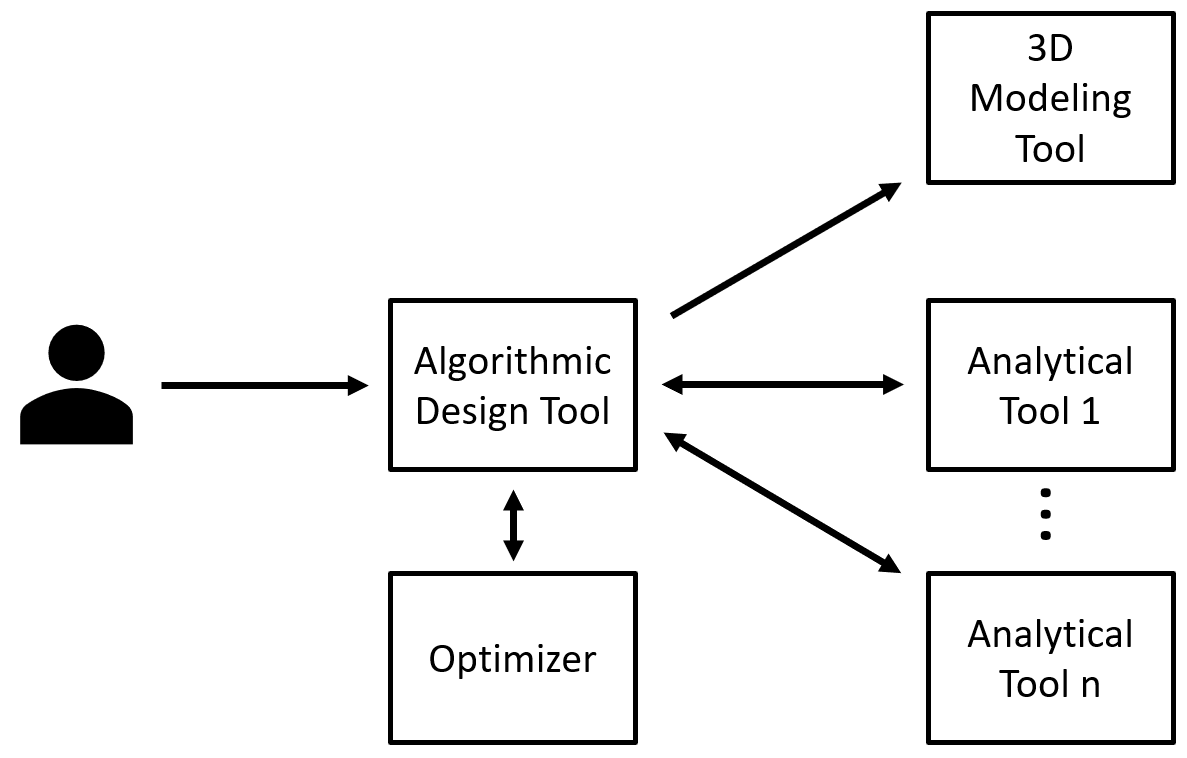
\includegraphics[width=0.6\textwidth]{./Images/Solution/algorithmic_optimization.png}
 	\caption[Algorithmic Optimization workflow]{Algorithmic Optimization workflow. In this workflow, the architect only interacts with an \ac{AD} tool to create the initial design, to specify the analysis tools, and to specify the optimization parameters.}
 	\label{fig:algorithmicoptimization}
 \end{figure}
 
In order to benefit from the \ac{AO} approach, we combine the optimization framework developed in this dissertation with an \ac{AD} tool to provide an alternative to easily address a wide variety of \ac{BPO} problems. To this end, architects are required to: (1) create the \ac{AD} model reflecting their design's intents; (2) select the performance aspects to optimize and, thus, the analysis tools to be used (e.g., lighting, thermal, structural, costs), and, finally, (3) to select, if necessary, the parameters of the optimization process (e.g., algorithm, algorithm's parameters). %In the end, architects are only required to run the script and the optimization process will automatically start. 
\Cref{BPOjuliaCode} presents a simple example of an \ac{AO} approach using the developed framework and the Khepri \ac{AD} tool, where the architect: (1) defines the algorithmic description of the intended design (\textit{lines 1-4}), (2) defines four variables and their acceptable variation range (\textit{lines 17-20}), (3) defines the objective functions for the performance aspects to consider in the optimization (\textit{lines 6-14 and 21-22}), (4) creates the optimization model (\textit{line 23}), (5) defines the algorithm's parameters (\textit{line 24}), and (6) specifies the optimization algorithm and the maximum number of evaluations (\textit{line 25}).

Even though the provided example presents a textual-based \ac{AO} approach, the developed optimization framework can easily be integrated within a visual \ac{AD} tool, like Grasshopper. 

One important aspect that results from this combination is the fact that architects are able to use different optimization algorithms and, consequently, to select an optimization algorithm that better suits their problems. To bridge the gap between the lack of knowledge or experience and the suitability of optimization algorithms for each problem, the optimization framework also provides automated testing mechanisms. These mechanisms enable the sequential execution of multiple optimization algorithms for a specified amount of evaluations, as well as each algorithm's performance measures. This feature is particularly important in the architectural context~\cite{Wortmann2016BBO,Hamdy2016}, as it promotes more informed decisions towards the selection of more appropriate optimization algorithms.


\begin{lstlisting}[caption={BPO example of the framework's API using the Khepri AD tool.},label=BPOjuliaCode]	
building_with_skylight(height, width, length, material) = let
	# Create the design using Khepri's primitives
	...
end

# Analytical-based criterium
cost(height, width, length, material) = let
	p1 = scale(width, 1.5) * scale(length, 6.5) * 185,
	p2 = (scale(width, 1.5) + scale(length, 6.5)) * 2 * height * 80
	p1 + p2
end

# Simulation-based criterium
daylight(height, width, length, material) = radiance_analysis(...)

# Optimization Process
let height = RealVariable(0.1, 2),
	width = RealVariable(0.1, 6.5),
	length = RealVariable(0.1, 11),
	material = IntVariable(0, 3),
	obj1 = Objective(daylight, :MAX),
	obj2 = Objective(cost, :MIN),
	model = Model([height, width, length, material], [obj1, obj2]),
	NSGA_params = Dict(:population_size => 10)
  solve(NSGAII, NSGA_params, model, max_evals=100)
end
\end{lstlisting}

Due to the visual nature of architects and the generalized lack of confidence in optimization processes, the visualization of evaluated design solutions is of great importance, as it allows architects to explore and corroborate the optimization results. To this end, the optimization framework provides post-processing and visual mechanisms (see \cref{fig:postprocessing}) that, when combined with an \ac{AD} tool, allow the architect to click on the evaluated solutions and instantly visualize the corresponding design in a 3D modeling tool. 

\begin{figure*}[htbp]
	\centering
	\subfigure[]{%
		\label{fig:postprocessing-a}%
		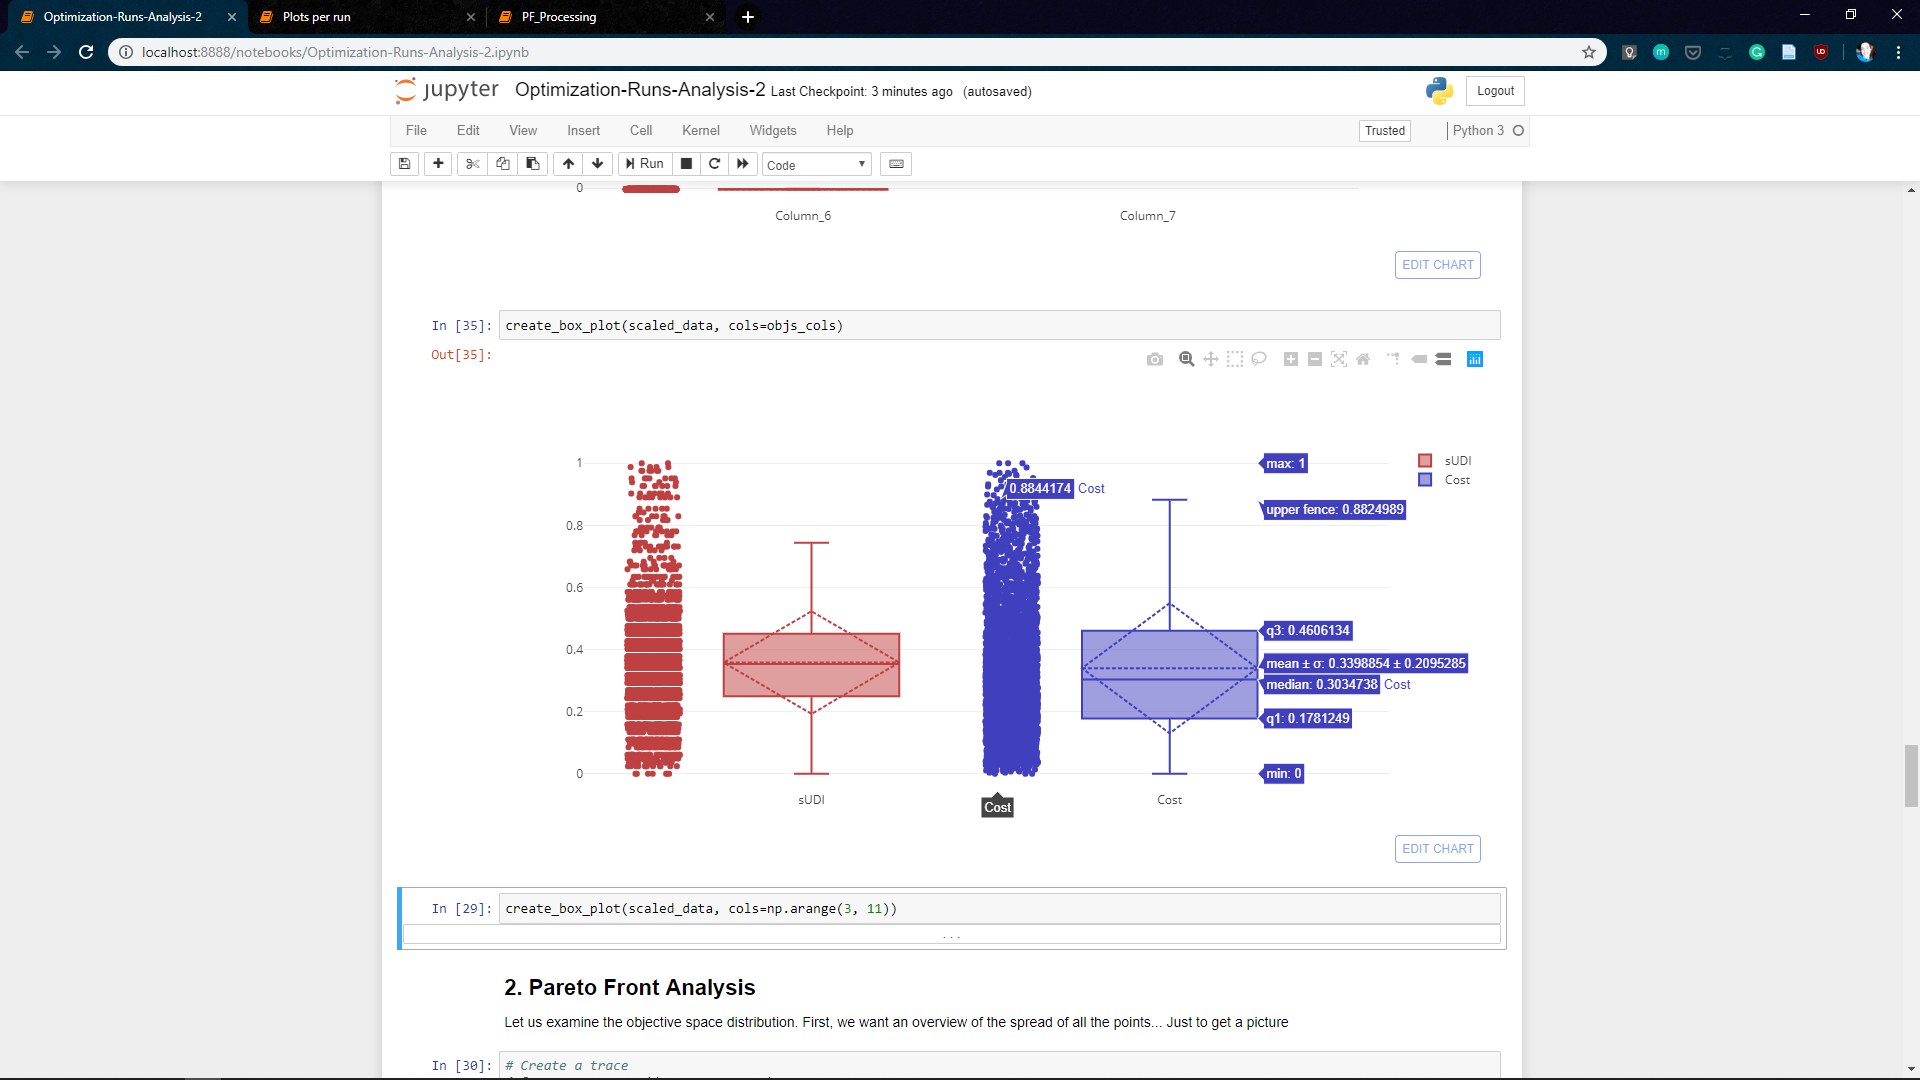
\includegraphics[width=0.485\textwidth]{./Images/Solution/postprocessing.png}}%
	\hfill
	\subfigure[]{%
		\label{fig:postprocessing-b}%
		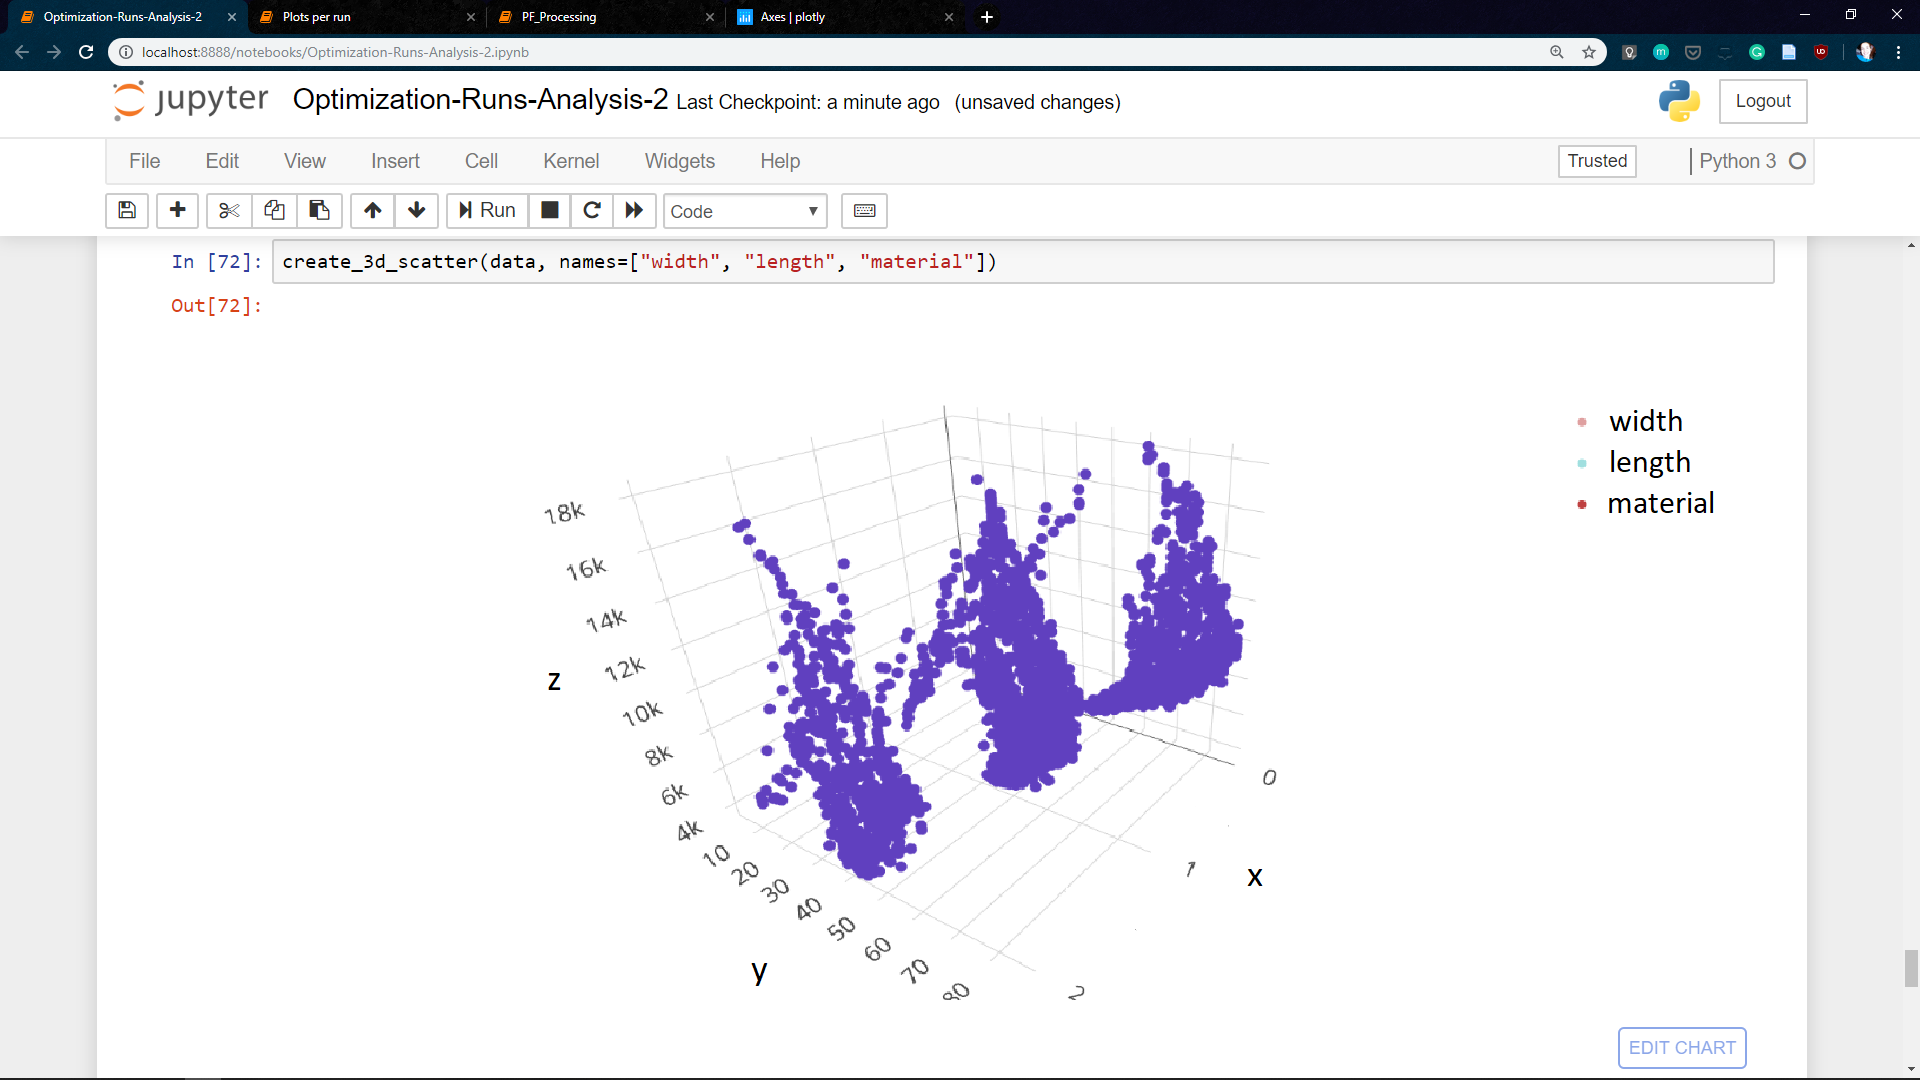
\includegraphics[width=0.485\textwidth]{./Images/Solution/postprocessing3-Copy.png}}%
	
	\caption[Examples of the post processing and visual mechanisms of the proposed solution]{Examples of the post processing and visual mechanisms (a) Box plot exhibiting the distribution of two objectives (b) 3D scatter plot of the variation of two objectives, $y$ and $z$, in function of the variable $x$.}
	\label{fig:postprocessing}
\end{figure*}

These visual mechanisms also promote a better comprehension of the optimization process, as they allow architects to explore and visualize the results of the optimization, in real-time, to get a clearer perspective. Besides reasoning and creating logical patterns that allow them to explain the obtained results, architects can also learn more about their designs' behavior regarding different performance aspects and, potentially, about the optimization algorithm itself.

Finally, visualization and processing mechanisms can also be useful not only to detect errors or incoherences (e.g., in the optimization model) early in the optimization process, but also to reduce the overall optimization time, i.e.,  provide the architect with enough information to stop the optimization process sooner. For some problems, obtaining an optimum is not strictly necessary. Instead, a close to optimal or good solution suffices. Having a framework which interactively updates the information about the optimization process is particularly useful for those problems, since the user can explore and visualize the already evaluated candidate solutions and decide whether one of them suffices, even if it is not an optimum. 

\section{Summary}
In this chapter, we explored the application of a general purpose optimization framework to \ac{BPO} problems, which frequently incorporate expensive simulation-based objective functions, ranging from a couple of seconds to a few days, depending on both the analysis domain and the design's complexity. Also, we described how the framework can be coupled with existing algorithmic-based approaches to promote the automation of optimization processes, an approach we named \ac{AO}.

To address the abnormal time-complexity associated with \ac{BPO} problems, we provide the architects with the ability to follow different optimization approaches (e.g., experimental, \ac{SOO}, \textit{a priori} preference articulation, Pareto-based), as well as with optimization algorithms specially tailored for addressing these problems more efficiently. These include model-based algorithms that significantly reduce the overall optimization time by using fast surrogate models for evaluation. %Moreover, our framework provides both global and local algorithms, thus providing the flexibility for obtaining either more or less precise solutions. 
%We aim at reducing the abnormal time-complexity of \ac{BPO} by providing model-based algorithms. 

To address the low feedback of the optimization process, we provided a set of files that keep track of every evaluated solution, hence enabling the user to freely access that information and use it for posterior optimization processes. Moreover, this information is enriched by providing integrated visualization features, which enable the view of the 3D model associated with an evaluated design solution. As a result, this promotes quicker and more informed decisions regarding the building design's practice.

It is important to mention that the discussed optimization framework is not limited to the visual programming paradigms like most competing tools and it can also be integrated within a textual programming paradigm. %When combined with the Khepri or Rosetta textual-based \ac{AD} tools, the framework benefits from their inherent portability and scalability properties. 

Finally, we reflect on the usability of the proposed solution. Unlike existing architectural optimization tools, our solution does not currently benefit from the friendliness of the visual paradigm. This can be an obstacle to its application in architectural practice, where architects often lack programming skills. To this end, we hid the underlying complexity of the optimization framework under a simple and intuitive abstraction layer. 

% To this end, we developed a simple and intuitive abstraction layer, even for non-programmers. As a result, we hide the complexity of the integration of several optimization libraries under an abstraction layer, providing a clean and succinct set of primitives. These primitives draw inspiration from simple optimization mathematical models and are rather intuitive and easy to use. 

% If Printing on DOUBLE SIDED pages, the second page should be white.
% Otherwise, comment the following command:
\cleardoublepage
%
%Chapter 5
% #############################################################################
% This is Chapter 4
% !TEX root = ../main.tex
% #############################################################################
% Change the Name of the Chapter i the following line
\fancychapter{Evaluation}
%\cleardoublepage
\label{chap:evaluation}
 
The main goal of this dissertation was to identify different optimization algorithms capable of handling the computationally complex problems that characterize \ac{BPO}, and to devise strategies for its efficient application to architectural design optimization problems. The goal included both single- and multi-objective optimization. To concretize this study, we proposed and implemented an optimization framework which enabled not only the application of different optimization approaches, but also to use several algorithms within each approach.  Finally, we claimed that the proposed framework allows architects to easily explore automated optimization processes within architectural practices. 

This chapter focuses on the evaluation of the proposed framework from both a qualitative perspective and a quantitative one. In particular, \cref{sec:qualitative} discusses the qualitative properties of the optimization framework, especially, for \ac{BPO} practices, outlining its advantages and disadvantages. On the other hand, \cref{sec:quantitative} tests different optimization algorithms, measuring their adequacy for different \ac{BPO} problems. Moreover, it also appraises the framework in the architectural practice through its application to different \ac{BPO} problems. To this end, we follow the algorithmic framework described in \cref{chap:implement}, which exploits the optimization framework described in \cref{chap:architecture} and the Khepri \ac{AD} tool. 

The evaluation aims to answer the following questions: 
\begin{itemize}
	%\item Do the studied algorithms present benefits for the architectural practice? 
	\item Is there a single algorithm that can consistently, across all case studies, reach the best solution?
	\item Is there any class or subclass of algorithms that constantly outperforms others?
	\item Can any of the algorithms reduce the impact of the expensive simulations typically performed in building design? 
	\item Is the proposed framework tailored for performing optimization in architectural practices? 
	\item How does the proposed framework benefit architectural practices?
\end{itemize}


\section{Qualitative Evaluation}
\label{sec:qualitative}

The qualitative evaluation of optimization frameworks involves considering multiple aspects, including the flexibility, adaptability, diversity of algorithms, ease of use, among others. Calling upon the No Free Luch Theorem (\ac{NFLT}) discussed in \cref{ssec:comparisondfo}, some algorithms are really good solvers for some problems and very poor solvers for others~\cite{Wolpert1997NFLT}. In fact, selecting the right algorithm can have a great impact in the efficiency of optimization processes. Particularly, in building design, to benefit from such performance gains, diversity of algorithms allows to face each problems' characteristics differently, enabling the identification of most promising algorithms. Besides the algorithms' diversity, in order to be easily used by less experienced users, algorithms should be effortlessly run, without the need for many manual changes. Notwithstanding their innate simplicity, optimization frameworks should also be flexible enough to enable more experienced users to fine-tune them, thus fostering more efficient optimization processes. At last, a good framework should adapt to handle different problems.

Regarding the adaptability of the proposed framework, it provides mechanisms to address both single- and multi-objective problems: 15 \ac{SOO} algorithms and 13 \acp{MOEA}, respectively. Simpler approaches, like the design of experiments approach discussed in \cref{ssec:doe}, are also possible using one of the 5 sampling methods available in the framework. Moreover, a core feature of this framework is that it provides 10 \ac{ML} algorithms to be combined with other algorithms, thus  promoting the potential reduction of the time complexity involved in building design. 

Back in \cref{chap:architecture}, we discriminated all the algorithms available in the framework (see \cref{table:algorithms}). When comparing to existing optimization tools in architecture, our solution presents a more extense and diverse set of algorithms, which can be explored to address a wider variety of problems. Moreover, while the existing tools rely on a unique optimization approach, such as \ac{SOO} approaches or Pareto-based optimization ones, the solution hereby proposed supports different approaches.

Unlike competing optimization tools, which are implemented on top of visual programming languages, like Grasshopper and Dynamo, our framework is currently implemented on top of a textual programming language. Although the visual paradigms' graphical feel provides a more comfortable experience to less experienced users, the fact that our framework makes use of the textual paradigm confers more scalability and portability.%, thus allowing users to seamlessly apply optimization to more complex buildings. 
Moreover, to make it more appealing to less experienced users, the developed optimization framework is setup as a ready-to-use tool, where every parameter of the optimization process is configured by default.  

Besides the ready-to-use format, the framework supports detailed configurations of the different algorithms, thus allowing more experienced users to fine-tune and, if desired, to combine different algorithms. 

Moreover, given the importance of testing different algorithms before settling for a single one~\cite{Wortmann2016BBO}, the developed framework provides the necessary mechanisms to facilitate the automated testing of multiple algorithms with no additional efforts for the users. Conversely, competing tools frequently require users' intervention to test different algorithms, either by dragging other optimizer components and making necessary changes in the design script or, when possible, by simply re-configuring the optimization tool to use one of the other supported algorithms. 

Regarding the post-processing and logging mechanisms, the proposed framework is automatically configured to produce complete log files, including all the information about the algorithms and problems being addressed, as well as a real-time log of the different solutions explored during the optimization run. This differs from existing architectural optimization tools, which only produce the log files after the execution. Nevertheless, some of the currently existing optimization tools still visually outperform the developed framework. In fact, while the current framework implementation seldom provides visual interactive Python scripts that read the log files and produce the corresponding plots, some of the existing architectural optimization tools already update the information of the optimization process in real-time. Note, however, that users are also able to visualize a more updated view of the optimization process as long as they re-run the visualization script. 

Finally, in order to use the optimization framework, users only need to create their design's parametric description and to model the corresponding optimization problem, which involves the definition of the variables and its bounds, of the objectives, and, if necessary, of the constraints. In contrast to the existing tools, which require the modification of the optimization script (e.g., drag other components, redefine the optimization problem, change the optimization tool), our framework requires no such efforts to use different algorithms and/or optimization approaches. Instead, users are only required to specify the algorithms that they wish to apply and to configure them accordingly.

\todo{Tabela sumarizar avaliação S:}

% #############################################################################
\section{Quantitative Evaluation}
\label{sec:quantitative}

In order to study and explore the effectiveness of algorithms within building design practices, we evaluated the performance of different algorithms using the optimization framework, discussed in \cref{chap:implement}. Moreover, we evaluated the real applicability of such framework in three case studies, two of which were proposed by an architectural studio\footnote{Atelier dos Remédios: http://atrem.eu/}: (1) the optimization of the lighting conditions of a solarium in a private house in Portugal; (2) the optimization of the structural behavior and elegance of an arc-shaped space frame structure; and (3) the optimization of the cost and the lighting conditions of an exhibition room in an urban museum.   

In order to measure the effectiveness of the optimization algorithms, different factors must be considered: (1) the optimization time is sensitive to the computational power of the machine where the algorithm is being run, (2) the non-determinism of several optimization algorithms, and (3) the hyperparameters of optimization algorithms. Firstly, to remove the time dependency of the machine characteristics and objective function's complexity, we measure the performance of the optimization algorithm in terms of the number of function evaluations, which is proportional to the actual time spent by the optimization process. Secondly, the stochastic character of several optimization algorithms (e.g., random modifications of solutions, random generation of design solutions, random initial points) might yield different results even when ran twice under the same configurations. To address this limitation, we run each stochastic algorithm three times and we use the average of the values to draw conclusions. Finally, an algorithm's performance for each problem can be better or worse depending on its configurations. To this end, we opt for using the default algorithm's configurations, thus emulating the case when the architect's knowledge does not suffice to properly fine-tune the algorithm. 

\todo{ESCLARECER diferença entre combined PFs, true PFs, Approximated PFs}
% #############################################################################
\subsection{Ericeira House: Solarium}
The first \ac{BPO} case study involved the optimization of the daylight conditions of a room in an isolated private house in Portugal~\cite{Caetano2018,Belem2018optimizeddesign}. The room was designed with a set of façade shading panels that modulate the daylight conditions on the interior of the room. The panels are composed of a set of horizontal wood bars of different sizes, which alternate between one full-length bar and a set of smaller bars. For aesthetics reasons, the size and position of the smaller bars along the panel's width were randomized. The final pattern of the façade's shading panels was defined in terms of the length’s step, the maximum distance separating two consecutive bars, and the minimum and maximum lengths of the smaller bars. Initially, the goal was to find a solution for the shading panels that maximized the room's daylight performance, which was measured using the \ac{sUDI} metric~\cite{Nabil2006}. While, in general, it is known that the more openings in the shading panels, the more daylight enter the room, this may also cause situations of uncomfortable glare. As a result, these situations should be accounted for, and, notwithstanding the values of the optimization process, architects should always perceive optimization results with a critical thinking. \Cref{fig:ericeira_multiple_panels} represents some design variations, ranging from denser patterns, with lower \ac{sUDI} values, to sparser ones, with higher \ac{sUDI} values.

%\begin{figure}[htbp]
%	\centering
%	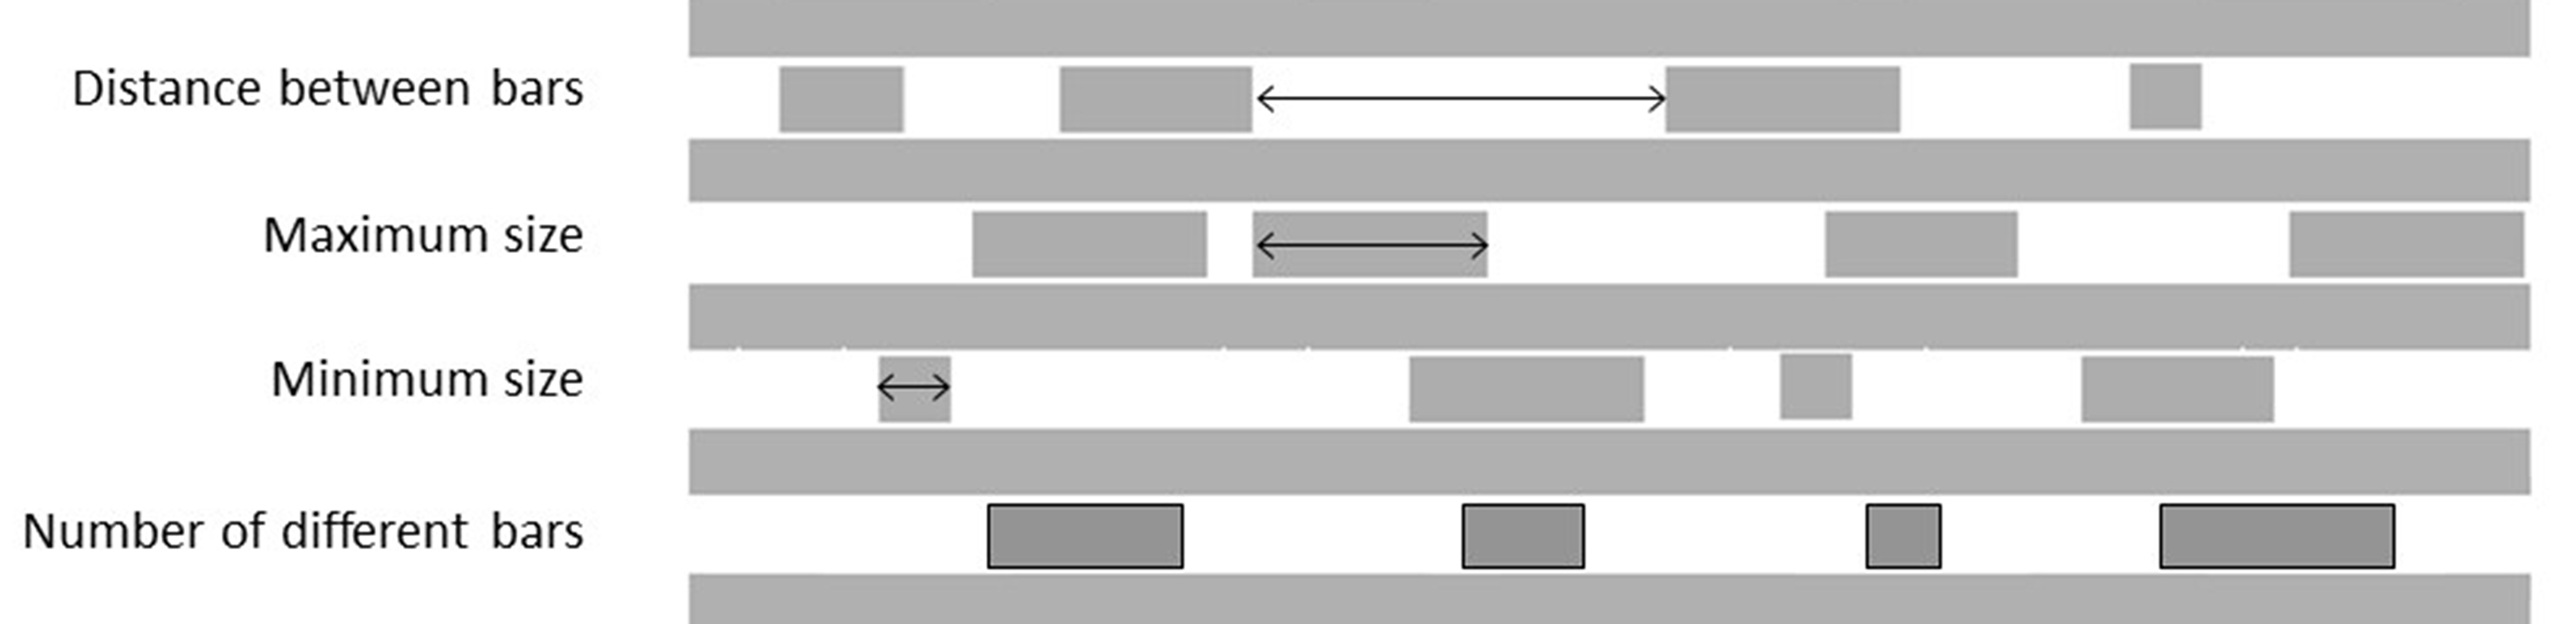
\includegraphics[width=\textwidth]{Images/Evaluation/Ericeira_1.jpg}
%	\caption{Ericeira Solarium: Representation of the shading panels' geometric pattern and design variables.}
%	\label{fig:ericeira_panels_explanation}
%\end{figure}

\begin{figure}[htpb]
	\centering
	\includegraphics[width=\textwidth]{Images/Evaluation/Ericeira_2.png}
	\caption{Ericeira Solarium: Representation of the shading panels’ geometric pattern with different sUDI values (from left to right, 7\%, 62\%, 90\%, and 100\%).}
	\label{fig:ericeira_multiple_panels}
\end{figure}

Initially, we pursued a simple design of experiments approach to address this optimization problem \cite{Caetano2018}. To generate the design variants to evaluate, we used the Monte Carlo and the latin hypercube sampling algorithms. Following such approach allowed us to exploit previous knowledge about the shading panels and its impact on the daylight conditions of the room (e.g., that sparser patterns increase daylight performance) and, consequently, to produce a more efficient optimization process. In fact, based on this knowledge, we set several iterations of the different sampling methods and, within each iteration, we have further restrained the variables' to vary in smaller ranges, thus enforcing the sampling of incrementally more efficient designs. %\Cref{fig:ericeira_doe} shows an example of the results obtained during this process, as well as the solutions that were presented to the architects, so that they would choose the one that better suited their intentions.

%\begin{figure}[htbp]
%	\centering
%	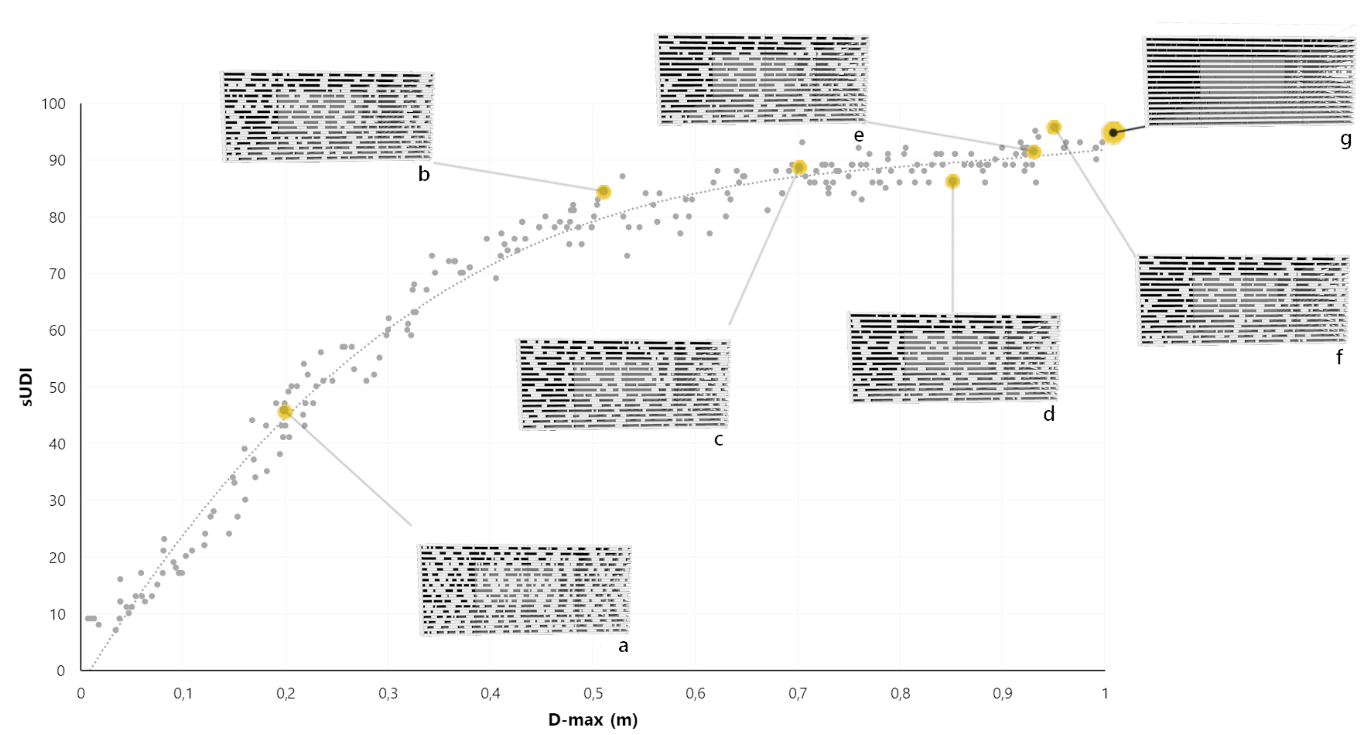
\includegraphics[width=\textwidth]{Images/Evaluation/Ericeira_caadria2018.PNG}
%	\caption{Ericeira Solarium: The scatter plot with the samples obtained during the design of experiments approach. The models a. to g. correspond to the set of examples presented to the architects.}
%	\label{fig:ericeira_doe}
%\end{figure}

Despite achieving optimal solutions with values of sUDI of $100\%$, we have only achieved these solutions after 200 function evaluations. Because each evaluation took approximately $7$ minutes to complete on dual \textit{Intel Xeon CPU E5-2670 @ 2.60GHz, 64GB RAM}, the optimal solution was only obtained after $1400$ minutes, or, equivalently, $23.33$ hours. This large time complexity resulted from the fact that approaches based on sampling algorithms consist on the consecutive uniformed experimentation of multiple designs, i.e., without taking into consideration previous design evaluations, often evaluating irrelevant design solutions. Moreover, this approach required several manual interventions (e.g., analyse the results, redefine the variables' bounds, select number of evaluations). In an attempt to minimize the time complexity of the optimization process and to verify the impact of more guided approaches in \ac{BPO} problems, we have also approached this problem using a \ac{SOO} approach \cite{Belem2018optimizeddesign}. Particularly, we evaluated the performance of $13$ different derivative-free optimization algorithms: $5$ direct-search, $3$ metaheuristics, and $5$ model-based. Given the time complexity of each function evaluation, we set a limit of $60$ function evaluations per run.

%http://papers.cumincad.org/data/works/att/caadria2018\_278.pdf
\begin{table}[htbp]
	\centering
	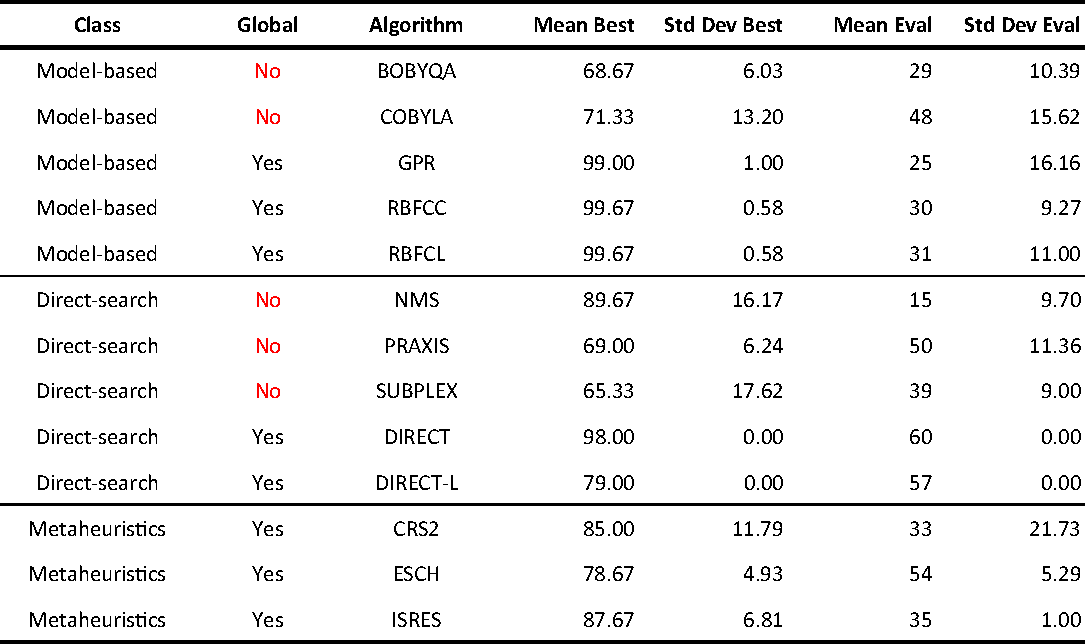
\includegraphics[width=\textwidth]{tables_and_code/Ericeira_phase1_stats_v1.pdf}
	\caption[Ericeira Solarium: Mean best results and evaluations discriminated per algorithm]{Ericeira Solarium: Table with the mean best daylight results and mean evaluations to reach optimal solutions of each algorithm. Results are averaged over $3$ runs, each with $60$ evaluations.}
	\label{table:phase1results}
\end{table}

\Cref{table:phase1results} shows the mean best results and the standard deviation of the $3$ runs,  discriminated by algorithm. According to the results, in average, the global model-based algorithms $GPR$, $RBFCC$, and $RBFCL$ were able to find an optimal solution within the first $30$ evaluations. Conversely, the local model-based algorithms $COBYLA$ and $BOBYQA$ performed rather poorly in this problem, converging to far from optimal solutions after $29$ and $48$ function evaluations, respectively. Regarding direct-search algorithms, the global algorithm $DIRECT$ was able to find a close to optimal solution (with an \ac{sUDI} value of $98\%$) in the last function evaluation. Its local variant, $DIRECT$-$L$, and the local direct-search algorithms $PRAXIS$ and $SUBPLEX$ fell short of the expected and barely managed to improve over $80\%$. Nevertheless, the simplex-based direct-search algorithm $NMS$ performed surprisingly well, having achieved an average result of $89.67\%$ within the first $15$ evaluations. Finally, although metaheuristics performed better than most local model-based and direct-search algorithms, they seem to stagnate in design solutions with \ac{sUDI} values below the $88\%$, after $30$ evaluations.

\Cref{fig:phase1results} shows the average performance per algorithm class, also separating them in local or global algorithms. Overall, local algorithms seem to perform worse than all other algorithms, with local direct-search and model-based algorithms stagnating towards design solutions with \ac{sUDI} values below $75\%$ and $70\%$, respectively. Contrastingly, global algorithms were able to find design solutions with values of \ac{sUDI} larger than $80\%$. Despite the good initial performance of metaheuristics algorithms for the first $20$ evaluations, global direct-search algorithms quickly surpassed them, achieving close to optimal solutions with \ac{sUDI} values of $90\%$. Lastly, global model-based algorithms were, on average, the best performing algorithms, achieving close to optimal solutions shortly after $24$ evaluations. 

\begin{figure}[htbp]
	\centering
	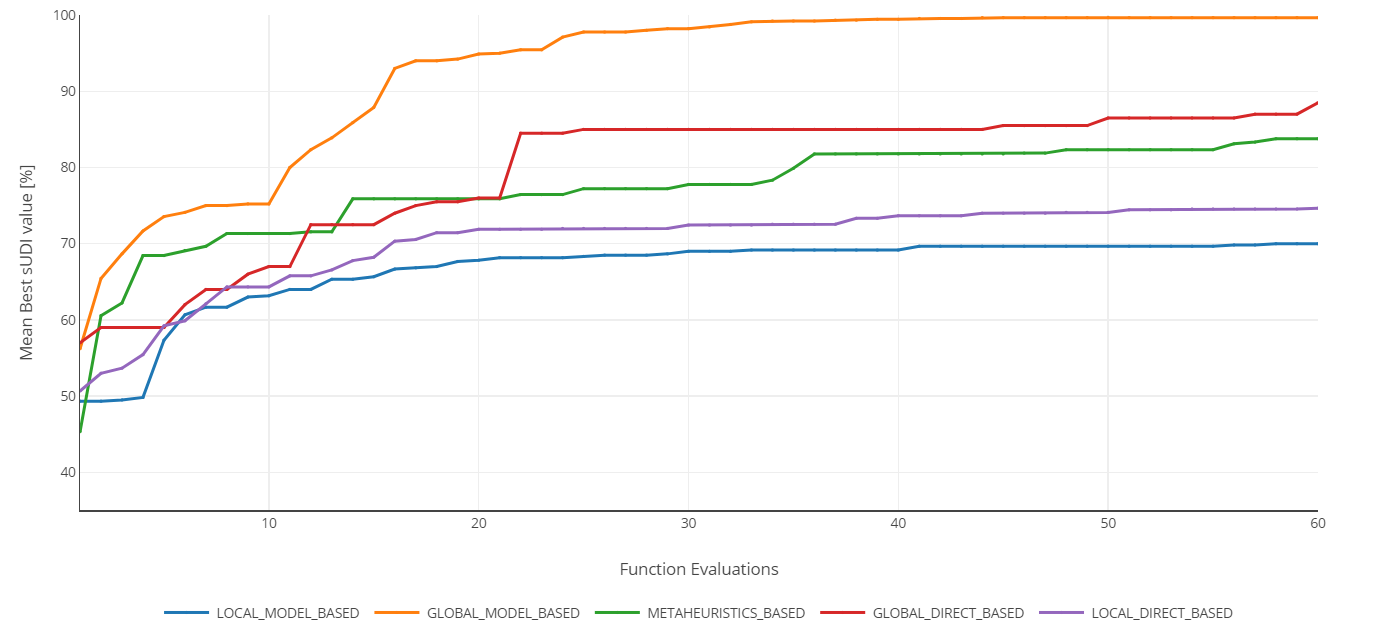
\includegraphics[width=1\textwidth]{Images/Evaluation/Ericeira_results_ph1_per_class.PNG}
	\caption[Ericeira Solarium: Mean best daylight results in function of the number of evaluations, discriminated per class of algorithms]{Ericeira Solarium: Mean best daylight results in function of the number of evaluations, discriminated per class of algorithms.}
	\label{fig:phase1results}
\end{figure}

Given the overall bad performance of local algorithms, we decided to assess their performance when submitted to different initial solutions. Notwithstanding their ability to quickly converge to locally optimal solutions, the quality of the found solutions highly depends on the solution used to initialize the search. As a consequence, we have also studied the impact of different initial solutions in the performance of these algorithms. To this end, we tested all $5$ local algorithms with two different initial solutions: a bad solution, with a $7\%$ value of \ac{sUDI}, and a reasonable solution with a $78\%$ value of \ac{sUDI}. Moreover, we decided to further restrict the number of evaluations to $15$, thus emulating an hypothetical scenario, where users lack knowledge about different optimization algorithms and, as a consequence, opt for testing several algorithms. Ideally, this test would allow them to infer the most promising algorithm and obtain a reasonable solution to hot-start other algorithms and, potentially, improve the overall optimization time.

\Cref{fig:phase2results} presents the mean best daylight results found by each local optimization algorithm. As expected, no local algorithm was able to obtain a good solution when provided with a bad starting solution. On the one hand, when provided with a mild initial design, both $COBYLA$ and $NMS$ found the best designs achieving a \ac{sUDI} value of $99\%$. On the contrary, $PRAXIS$ found the worse, and showed no relevant improvement over the initial design in terms of daylight illuminance. Nevertheless, it initially managed to outperform other methods, achieving values of \ac{sUDI} of $80\%$. After $8$ evaluations, $COBYLA$ and $NMS$ quickly converged to near optimal designs, with \ac{sUDI} values of $99\%$ and $98\%$, respectively. $BOBYQA$ and $SUBPLEX$ struggled to improve from the initial design.

On the other hand, when provided with a bad initial design, the best daylight result has an \ac{sUDI} value of $15\%$ and was found by $NMS$ after $9$ evaluations. $NMS$, $COBYLA$, and $SUBPLEX$ exhibit similar performance, stagnating in a design with an \ac{sUDI} value of $11\%$ after $3$ evaluations, with $NMS$ being able to further improve the design after $5$ evaluations. $PRAXIS$ exhibits the worst performance among all methods, showing no significant improvements throughout the whole optimization process.

\begin{figure}[htbp]
	\centering
	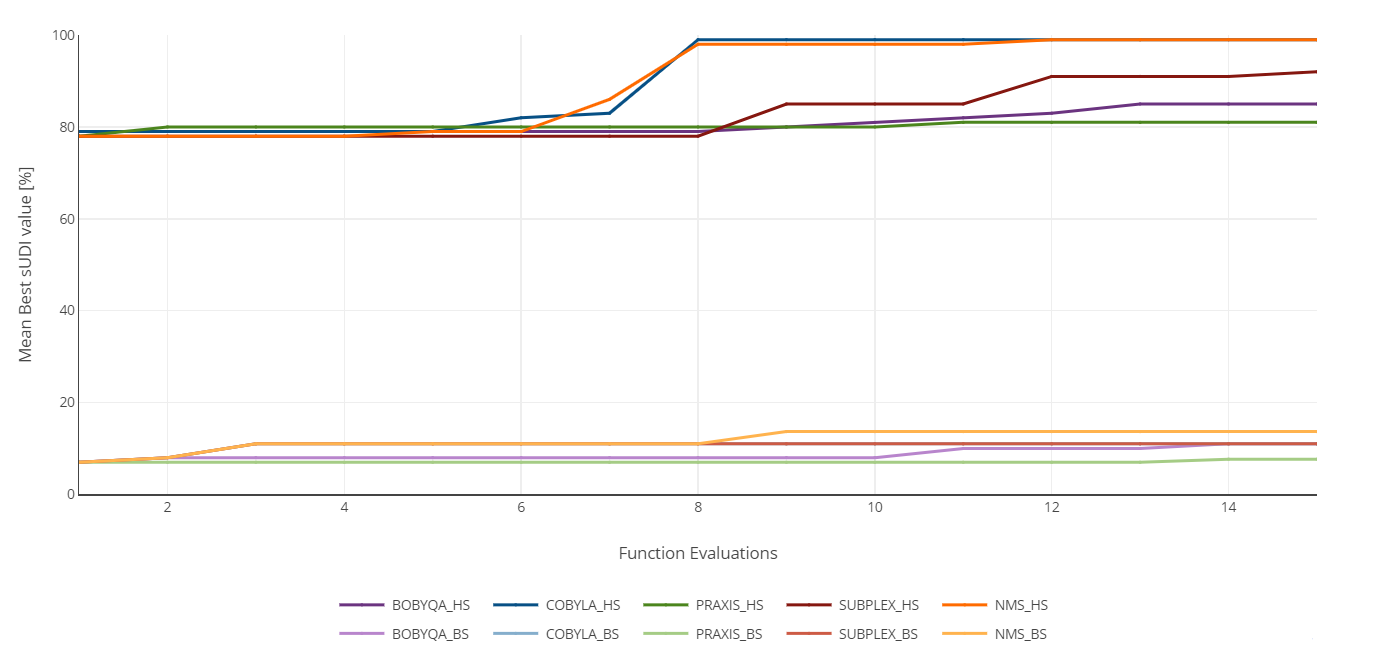
\includegraphics[width=\textwidth]{Images/Evaluation/Ericeira_results_ph2.PNG}
	\caption[Ericeira Solarium: Mean best results of daylight performance in function of the number of evaluations, discriminated per local algorithm]{Ericeira Solarium: Mean best results daylight results as a function of the number of function evaluations, discriminated per local algorithm. Algorithms suffixed with $HS$ are given an initial solution with an \ac{sUDI} value of $78\%$, whilst algorithms suffixed with $BS$ are given an initial solution with an \ac{sUDI} value of $7\%$.}
	\label{fig:phase2results}
\end{figure}


% #############################################################################
\subsection{Space Frame Optimization}

In this section, we address the first of two \ac{MOO} problems \cite{Belem2019MOO,IP2019MOO}. Motivated by the interest of architects in performing structural analysis \cite{Cichocka2017SURVEY}, the first case consisted in the optimization of both the structural behavior and an \textit{ad-hoc} measure of irregularity of an arc-shaped space frame. To instil irregularities in this space frame, we introduced three attractors that cause a deformation in the shape of the truss, each of which is defined in terms of its fixed-radius cylindrical coordinates in the arc-shaped space frame~\cite{Belem2019MOO}. To measure the goals for each design variant, we used (1) the Robot analysis tool to compute the maximum displacement of the structure, and (2) the sum of the Euclidean distances between the attractors. To increase the interest of this case study, we set out to minimize both objectives, thus promoting the conflict between them: placing the attractors near each other will weaken the structure and, thus, increase the maximum displacement of the space frame. In fact, to reduce the maximum displacement, the attractors should be scattered across the space frame but this implies larger distances among the three attractors and, thus, a less interesting shape. \Cref{fig:spaceframe} illustrates three examples of the space frame structure. 

\begin{figure}[htbp]
	\centering
	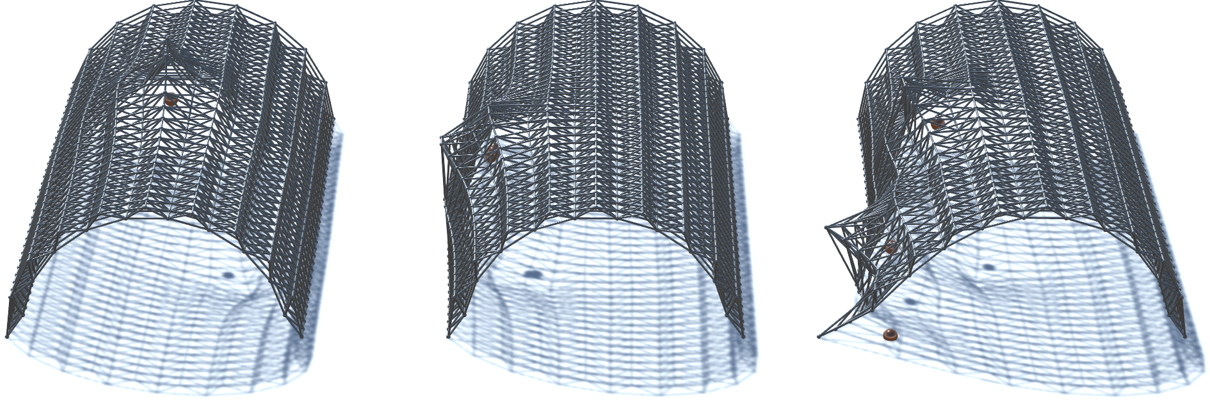
\includegraphics[width=1\textwidth]{Images/Evaluation/truss-kat-small.png}
	\caption[Space Frame: Representation of three space frame design variants]{Space Frame: Representation of three design variations of the arc-shaped space frame, with copper balls representing the three attractors.}
	\label{fig:spaceframe}
\end{figure}

To optimize the space frame, we decided to test $10$ metaheuristics and $9$ model-based algorithms. On the one hand, each metaheuristic algorithm comprised a total of $15$ individuals/particles per iteration, which were evolved for $15$ iterations. On the other hand, model-based algorithms derived $100$ initial samples using the latin hypercube sampling algorithm, which were then used to create the initial approximation to the expensive evaluation function, upon which another $125$ evaluations were completed. Overall, every algorithm was limited to a total of $225$ function evaluations, each taking approximately $40$ seconds to complete on dual \textit{Intel Xeon CPU E5-2670 @ 2.60GHz, 64GB RAM}. 

The evaluation of these algorithms consisted in the computation of different performance indicators discussed in \cref{ssec:performance}, some of which required a reference set to be compared with. Ideally, this reference set would represent the true Pareto front in order to obtain a more fine-grained measure of each algorithm's performance. However this is not possible and, to better approximate the true Pareto front, we determined for each run the set of optimal solutions, which we named the combined Pareto front. Each run is composed of $4275$ candidate solutions. Afterwards, in an attempt to measure the average performance of each algorithm, we computed several performance indicators for each run, using as reference set the combined Pareto front of each run. Although this does not represent an accurate approximation to true Pareto front, we aim at measuring the average performance of each algorithm. To overcome this limitation, the algorithms should be allowed to run for thousands of iterations instead of a few hundreds. Unfortunately, time is frequently a limiting factor in \ac{BPO} problems, and, as a consequence, in the absence of the information about the true Pareto front, we have adopted a methodology similar to the one used for \ac{SOO}, which quantifies the performance of each algorithm in terms of the average of the different runs. 

\Cref{table:spaceframe,table:spaceframestd} show the mean results of the performance indicators and corresponding standard deviations for the three runs, discriminated by class and subclass. Since we are addressing a \ac{MOO} problem, we measured each algorithm's results in terms of several performance indicators. These indicators provide information about the three different relevant aspects of Pareto fronts: (1) the cardinality, measured by \ac{ONVGR} and \ac{ER}; (2) the diversity, measured with Spacing and Maximum Spread (named \textit{Max Spread} in the tables); and (3) accuracy/convergence, measured with \ac{MPFE} and \ac{GD}. Moreover, we a Pareto-compliant indicator, the \ac{HV}, to obtain a combined measure of all the three aspects mentioned. % To simplify the performance comparison among the different algorithms, we restrained the set of indicators to the unary ones. 
% 1 - Two set coverage não ia dar medidas relevantes porque raramente as diferentes frentes se tocam. 
% 2 - Epsilon indicators poderia ser interessante, mas não foi testada a implementação
% 3 - R-metrics requer funções de utilidade que não temos e que requer alguma sensibilidade em relação ao problema...

% The overall cardinality of each combined Pareto front is 14, 24, and 19, respectively.
When considering the cardinality aspect, the \ac{ONVGR} column of \cref{table:spaceframe} presents the optimal solutions ratio between each algorithm and the combined Pareto fronts. In general, metaheuristics seem to retrieve the most nondominated solutions within each run, whereas model-based algorithms seem to retrieve the least. In fact, among the model-based algorithms, the algorithms exploring random search strategies, i.e., the algorithms suffixed with $Random$, yield fewer nondominated solutions, which may result from a poor exploration of the solution space. On average, the best performing algorithm, $PAES$, is able to find twice the number of solutions that compose each combined Pareto front, whereas model-based algorithms, including $GPR$+$Random$ and \acp{MLP} algorithms, struggled to find a set of optimal solutions with at least half of the size of the combined Pareto fronts. 

%http://papers.cumincad.org/data/works/att/caadria2018\_278.pdf
\begin{table}[h!]
	\centering
	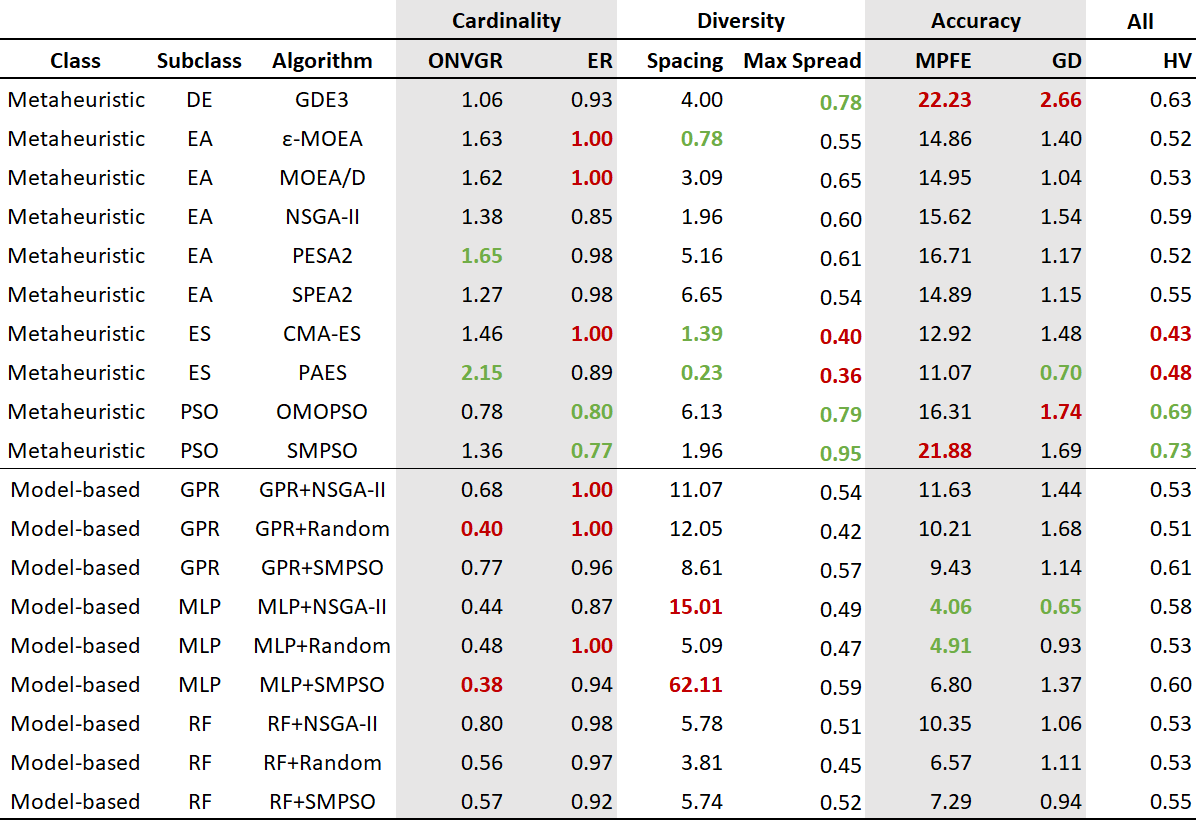
\includegraphics[width=\textwidth]{Images/Evaluation/caadria/Results_Mean_20190428.PNG}
	\caption[Space Frame: Mean values for the performance indicators results, discriminated per algorithms]{Space Frame: Mean values for the performance indicators results, discriminated by algorithm. Results are averaged over $3$ runs, each with $225$ evaluations.}
	\label{table:spaceframe}
\end{table}

While the \ac{ONVGR} indicator provides an intuition about the richness of the algorithms' Pareto fronts, many of the identified solutions might not be truly optimal, i.e., despite being optimal among all the evaluated solutions, these solutions might not belong to the true Pareto front or, in this case, to the combined Pareto front of the corresponding run. To this end, \ac{ER} is used to measure the percentage of false-optimal solutions for each algorithm. In this case, it becomes clear that even though $PAES$ retrieves twice as many optimal solutions as the combined fronts, most of them are not truly optimal. Moreover, none of the solutions found by the $\epsilon$-$MOEA$, $MOEA$/$D$, and $CMA$-$ES$ metaheuristics algorithms belong to the combined front. The same happens with some of the model-based algorithms, particularly, $GPR$+$NSGA$-$II$, $GPR$+$Random$, and $MLP$+$Random$. On the other hand, \ac{PSO}-based metaheuristics algorithms, $SMPSO$ and $OMOPSO$, exhibit the lowest \ac{ER} value, having found at least one true optimal solution in each run (see \cref{appendix:appendixB} for a more detailed view over the results of the three runs).

The diversity aspect consists in the analysis of the distribution of the nondominated solutions across the objective space. The Spacing indicator measures the uniformity of the set of optimal solutions retrieved by each algorithm, regardless of the combined Pareto front. Considering this indicator, the two \ac{ES}-based metaheuristic algorithms, $PAES$ and $CMA$-$ES$, and one \ac{EA}-based metaheuristic algorithm, $\epsilon$-$MOEA$, achieved the most uniform Pareto fronts. Conversely, model-based algorithms seem to yield more irregular Pareto fronts, namely, $MLP+NSGA-II$ and $MLP+SMPSO$ achieved the worst values of the Spacing indicator. Note, however, that this indicator merely provides an idea of the regularity of distribution of the solutions. Ideally, this indicator would also suggest a good coverage of the combined Pareto front, i.e., that the Pareto front found by each algorithm covers the same regions as the combined Pareto front, instead of focusing on a single smaller region. However, most of the algorithms which present the best scores in the Spacing indicator achieve such values because most of the identified optimal solutions lie within the same small region in the solution space, thus yielding a more uniform distribution. Additionally, these indicators are highly sensitive to outliers and to the number of retrieved solutions. % number of solutions also indirectly contributes to these scores of each indicators, since these indicators measure the distances between consecutive optimal solutions and the weight each outlier has in smaller or larger sets can greatly influence the final result.

Besides having an uniform distribution, when applicable, a good Pareto front should also cover large extents of the objective space in order to provide more relevant trade-offs. The \textit{Max Spread} indicator measures the extent of the Pareto fronts retrieved by each algorithm. On average, $SMPSO$, $GDE3$, and $OMOPSO$ are able to explore wider extents of the solution space. Observing \cref{table:spaceframe}, we conclude that, on average, $SMPSO$, $GDE3$, and $OMOPSO$ were able to cover the objective space better. Contrastingly, the \ac{ES}-based algorithms were the worst algorithms in this aspect, having explored smaller regions of the objective space. Regarding model-based algorithms, it is possible to observe that the ones based on $SMPSO$ were able to explore broader regions of the objective space than the ones based on $NSGA$-$II$ or $Random$ strategies. 

\begin{table}[]
	\centering
	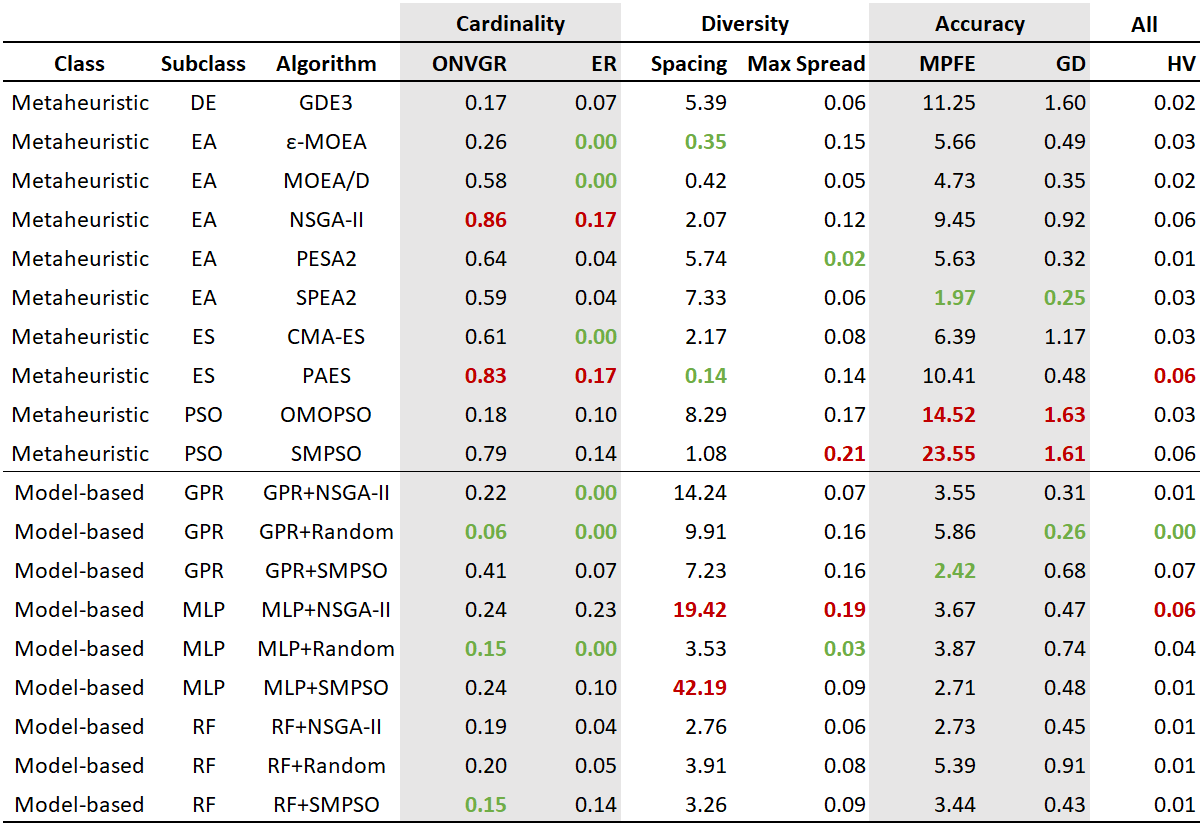
\includegraphics[width=\textwidth]{Images/Evaluation/caadria/Results_Std_20190428.PNG}
	\caption[Space Frame: Standard deviation values for the performance indicators results, discriminated by each algorithm]{Space Frame: Standard deviation values for the performance indicators results, discriminated by algorithm. Results are averaged over $3$ runs, each with $225$ evaluations.}
	\label{table:spaceframestd}
\end{table}

Another important aspect of Pareto fronts is their accuracy and how close their solutions are from the true Pareto front. As previously mentioned, in this dissertation, we consider the true Pareto front to be the result of the best solutions found in each run. This decision aims at measuring the average performance of each algorithm even when the real true Pareto front is unknown. In this case study, we used two accuracy indicators, \ac{MPFE} and \ac{GD}. On average, when considering \ac{MPFE}, every model-based algorithm retrieved Pareto fronts, whose \ac{MPFE} values were always better than the ones obtained by any metaheuristic. In particular, $MLP$+$NSGA$-$II$ and $MLP$+$Random$ have the smallest maximum error which means that all the points are at most at that distance from an optimal solution. Furthermore, the algorithms exploring a larger extent of the objective space, i.e., with higher values of Max Spread, have worse \ac{MPFE} values. This can be explained due to the lack of information about the true Pareto front, which is only approximated by the best solutions found in each run. 

Notwithstanding the fact that \ac{MPFE} provides an estimate of the maximum error of the algorithms' results, this indicator does not provide a real measure of how close the results are to the combined Pareto front. To this end, we use the \ac{GD} indicator, which measures the average approximation of the Pareto fronts retrieved by each algorithm to the closest solutions in the combined Pareto front. \Cref{table:spaceframe} shows that, on average, $MLP$+$NSGA$-$II$ and $PAES$ present the best convergence towards the combined Pareto front, and that $GDE3$ and $OMOPSO$ present the worst convergence values. These can be explained by the number of the nondominated solutions retrieved by each algorithm, as well as by the creation of clusters of optimal solutions near the combined Pareto fronts that were discovered by $PAES$ and $MOEA$/$D$, as is visible in \cref{sec:spaceframeoptimizationextra}. In general, other model-based algorithms also present reasonable scores, like the $MLP$+$Random$ or all the \ac{RF}-based algorithms even surpassing many metaheuristics algorithms, including $CMA$-$ES$, $\epsilon$-$MOEA$, $NSGA$-$II$, and $SPEA2$, thus suggesting better approximations.

In the end, we also used the \ac{HV} indicator, as it provides a general view over the quality of a Pareto front with regards to all three aspects simultaneously. The best performing algorithms were the \ac{PSO}-based algorithms, $SMPSO$ and $OMOPSO$, followed by $GDE3$. Surprisingly, the \ac{PSO} model-based algorithms also present a good performance, when compared to other metaheuristics, and even to other model-based algorithms that explore $Random$ or \ac{EA} strategies during the search for optimal solutions. On the other hand, the worst performing algorithms were the \ac{ES}-based ones, $CMA$-$ES$ and $PAES$, followed by $GPR$+$Random$. % Finally, comparing different algorithms regarding \ac{IGD}, the \ac{PSO}-based metaheuristic algorithms still yielded the best results, whilst \ac{ES}-based metaheuristic algorithms yielded the worst. However, $MOEA$/$D$ unexpectedly reveals itself as the third best performing algorithm when considering the \ac{IGD} indicator. Although this seems odd, this value can be explained by the difference in the scales of both axis and to the higher density of Pareto optimal solutions in the $x$-axis for values between $1.2$ and $1.3$.

\begin{figure}[htbp]
	\centering
	\includegraphics[width=\textwidth]{Images/Evaluation/caadria/All_Algorithms_all_runs-2019-04-13_1000dpi.png}
	\caption[Space Frame: Pareto front plot]{Space Frame: Line plot of the Pareto fronts retrieved by each algorithm measuring the Attractors distance in function of the Maximum displacement. These fronts are obtained by combining the values of the $3$ runs for each algorithm. The combined Pareto front is formed by finding the nondominated solutions from all the evaluated solutions.}
	\label{fig:allruns}
\end{figure}

Overall, no single algorithm was able to outperform the others in terms of all the indicators. Nevertheless, the \ac{PSO}-based metaheuristics algorithms, $OMOPSO$ and $SMPSO$, exhibited the overall best performance. Moreover, even though none of the model-based algorithms was able to surpass the $SMPSO$ and $OMOPSO$, the model-based algorithms that use $SMPSO$ also exhibited a reasonable performance, better than several well-known metaheuristics, including $\epsilon$-$MOEA$, $MOEA$/$D$, $CMA$-$ES$, and $SPEA2$. \Cref{fig:allruns} presents a combined view of all the algorithms for every run, where it is possible to visualize the extent of \ac{PSO}-based algorithms and the high density region to which several \acp{EA} and \acp{ES} algorithms converged.


\subsection{Black Pavilion: Skylights Optimization}
This case study addresses a real design problem where a two floor service building, called black pavilion, located in an urban context, is intended to work as a museum~\cite{Caetano2018,IP2019MOO}. Proposed by an architectural studio, the goal of this case study is to incorporate a skylight in the second floor of the building to improve the daylight conditions of an art exhibition space. Besides improving the daylight conditions of the exhibition space, the architects also intended to reduce the corresponding costs, thus prompting the optimization of two conflicting goals. Initially, the problem was to find the height, the width, the length, and the material of the skylight that maximized the daylight conditions and minimized the cost of the skylight, measured using the \ac{sUDI} metric~\cite{Nabil2006} and \cref{eq:costanalysis}, respectively. In \cref{fig:blackpavilion}, we present an example of the exhibition space and the daylight incidence that results from placing the skylight in the ceiling.

\begin{equation} \label{eq:costanalysis}
cost\_function(width, length, height) = (width * length * 185) + ((width + length) * ( 2 * height) * 80)
\end{equation}

Architects' previous knowledge did not suffice to determine the optimal configurations for the skylight. In general, it is known that the creation of higher skylights incur more costs and worse daylight conditions, as, in this case, higher skylights imply more direct light towards smaller areas in the exhibition space. Therefore, the team of architects fixed the height to be $1.5$\metre. Also, taking into account the fabrication costs, the team constrained the width and length to vary in multiples of $0.1$\metre. As a result, instead of modeling continuous variables, these were modeled as discrete variables.

\begin{figure}[htbp]
	\centering
	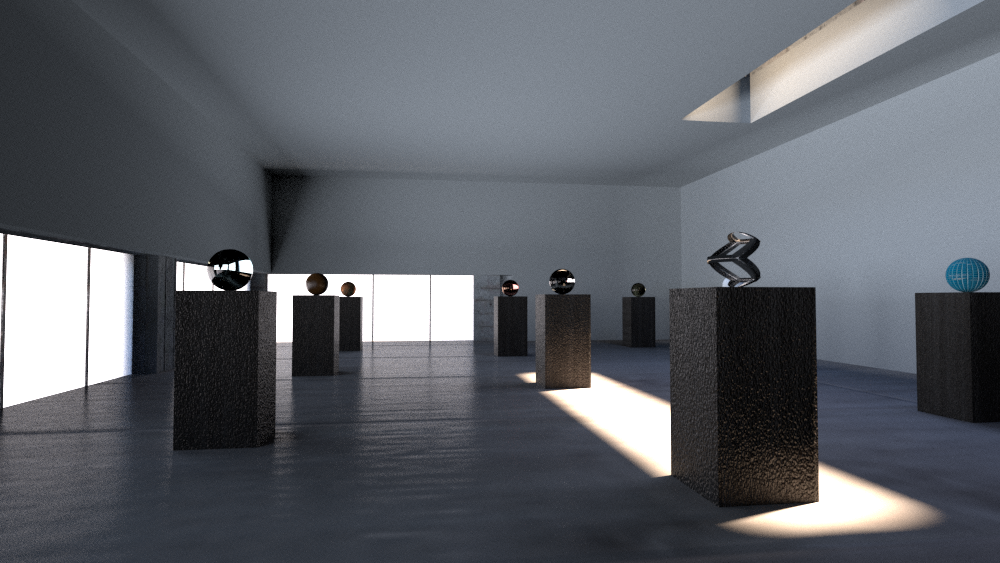
\includegraphics[width=\textwidth]{Images/Evaluation/BlackPavilion/PavPretoExample116x7204.png}
	\caption[Black Pavilion: Representation of the arts exhibition space with a skylight]{Black Pavilion: Representation of the arts exhibition space with the skylight in the top right corner.}
	\label{fig:blackpavilion}
\end{figure}

To this end, we conceived an algorithmic description of the building using the Khepri \ac{AD} tool and we used the Radiance lighting analysis tool to measure the \ac{sUDI} of different designs. Regarding the optimization, we decided to measure the performance of $10$ \acp{MOOA} regarding several indicators. Similarly to the previous case study, we aim at providing an average prediction of the behavior of each algorithm in this specific problem. As a result, we derived the combined Pareto fronts for each run and used them to compare the different algorithms. Each run comprises $200$ function evaluations, each of which takes on average $13.33$ minutes on dual \textit{Intel Xeon CPU E5-2670 @ 2.60GHz, 64GB RAM}.

Among the available algorithms and due to time constraints, we have selected $4$ metaheuristics, due to their acknowledged performance in other engineering applications: two \ac{EA}, $SPEA2$ and $NSGA$-$II$, and two \ac{PSO}, $SMPSO$ and $OMOPSO$. Additionally, we tested $6$ model-based algorithms, including $RF$+$Random$, $RF$+$NSGA$-$II$, $RF$+$SPEA2$, $GPR$+$Random$, $GPR$+$NSGA$-$II$, and $GPR$+$SPEA2$. \Cref{table:blackpavilion} shows the mean results of each algorithm for each of the evaluated performance indicators. 

\begin{table}[htbp]
	\centering
	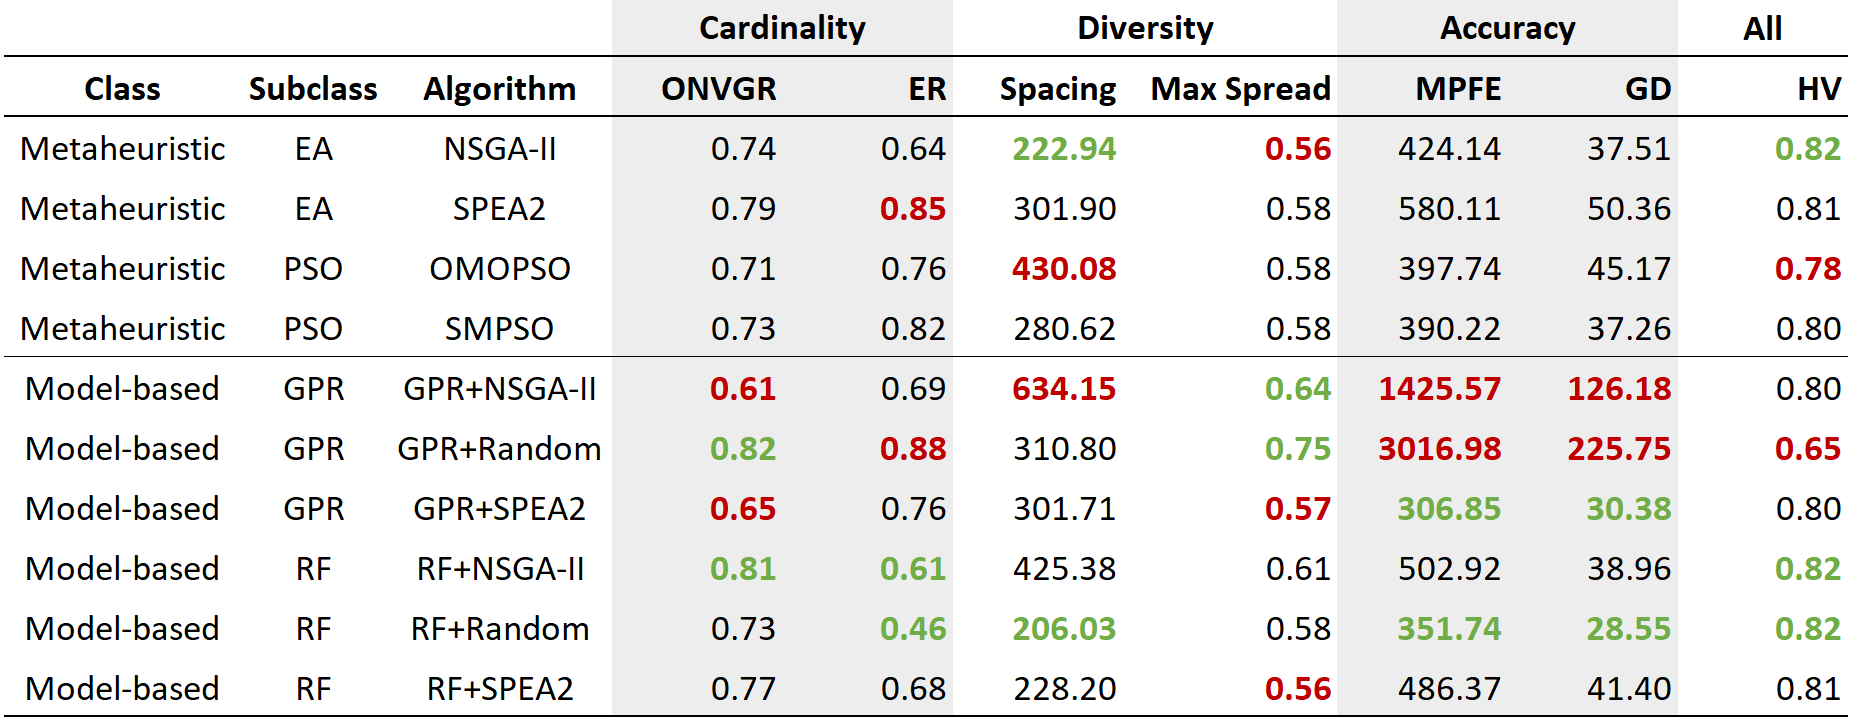
\includegraphics[width=\textwidth]{Images/Evaluation/BlackPavilion/Results_Mean_20190428.PNG}
	\caption[Black Pavilion: Mean values for the performance indicators results, discriminated by algorithm]{Black Pavilion: Mean values for the performance indicators results, discriminated by algorithm. Results are averaged over $3$ runs, each with $200$ evaluations.}
	\label{table:blackpavilion}
\end{table}

\todo{REVIEW}
Firstly, regarding the cardinality aspect of the results, all algorithms exhibit a \ac{ONVGR} value inferior to $1$, which means that no algorithm was able to retrieve as many optimal solutions as the combined Pareto front. Nevertheless, $GPR$+$Random$ and $RF$+$NSGA$-$II$ achieved the best results, attaining, on average, more solutions than all other algorithms. Conversely, $GPR$+$NSGA$-$II$ and $GPR$+$SPEA2$ obtained fewer solutions and were, therefore, the worst algorithms. Even though $GPR$+$Random$ retrieved the mean highest number of solutions, note that this value is subject to large variations, as evidenced in \cref{table:blackpavilionstd}, and, in fact, when examining the results per run, $GPR$+$Random$ retrieved $13$, $14$, and $24$ solutions. Regarding metaheuristic algorithms, \acp{EA} have achieved relatively higher cardinalities than \acp{PSO}. 

Notwithstanding the cardinality of the retrieved Pareto fronts, it is important to determine how many of these solutions actually lie in the combined Pareto front, which is measured by the \ac{ER} indicator. In this case, $RF$+$Random$ presents an \ac{ER} value less than $0.5$, which means that, on average, more than half of the retrieved solutions lie in the combined Pareto front. The second and third best performing algorithms were $RF$+$NSGA$-$II$ and $NSGA$-$II$ with values of $0.61$ and $0.64$, respectively. Conversely, $SPEA2$ and $GPR$+$Random$ presented the worst \ac{ER} values. Interestingly, even though $GPR$+$Random$ returned on average more solutions than all other algorithms, it barely succeeds in retrieving one optimal solution lying in the combined Pareto Front.

Secondly, when considering the dispersion of the solutions found by the algorithms in the objective space, $RF$+$Random$ and $NSGA$-$II$ exhibit the first and second best results. On the other hand, $GPR$+$NSGA$-$II$ presents the mean worst Spacing value, hence suggesting that the solutions retrieved by this algorithm are not evenly spread across the objective space. While $OMOPSO$ presents the mean second worse performance in terms of the Spacing indicator, this result is associated to a large deviation, which derives from the fact that in the third run the algorithm was able to retrieve a more uniform distribution (see \cref{sec:blackpavilionextra}). Interestingly, $RF$+$NSGA$-$II$, presenting the third worse Spacing value, also presents a large standard deviation. Upon a careful review over this algorithm's Pareto fronts for each run, this variation is explained due to a single solution in the second run that is offly distant from all others, which highly influences the results. 

When considering the maximum extent of the Pareto fronts discovered by each algorithm, i.e., the \textit{Max Spread}, $GPR$+$Random$ and $GPR$+$NSGA$-$II$ are the most performing algorithms, achieving values of $0.64$ and $0.75$, respectively. Conversely, the other \ac{GPR}-based algorithm, $GPR$+$SPEA2$, achieved the second worse performance with a value of $0.57$, only surpassing the performance of $NSGA$-$II$ and $RF$+$SPEA2$, whose value was $0.56$. 

Thirdly, we measured the mean accuracy of the Pareto fronts retrieved by each algorithm. In terms of the \ac{MPFE} indicator, $GPR$+$SPEA2$ deviates the least from the combined Pareto front, with a value of $306.85$ for the furthest solution. The second best algorithm is also a model-based algorithm, $RF$+$Random$, whose furthest found solution lies on average within $351.74$ from the combined Pareto front. The third and fourth best performing algorithms were \ac{PSO}-based algorithms, which achieved close to optimal solutions as well. Conversely, $GPR$+$NSGA$-$II$ and $GPR$+$Random$ achieved the worst results in terms of \ac{MPFE}, identifying nondominated solutions at a distance of $1425.57$ and $3016.98$ from the closest solution in the corresponding combined Pareto fronts. A noteworthy observation is that while the worse performance of $GPR$+$Random$ results mainly from its poorer performance during the second run (see \cref{sec:blackpavilionextra}), the same does not happen with $GPR$+$NSGA$-$II$, whose \ac{MPFE} results for the first and third run remain approximately on $1600$. 

\begin{table}[htbp]
	\centering
	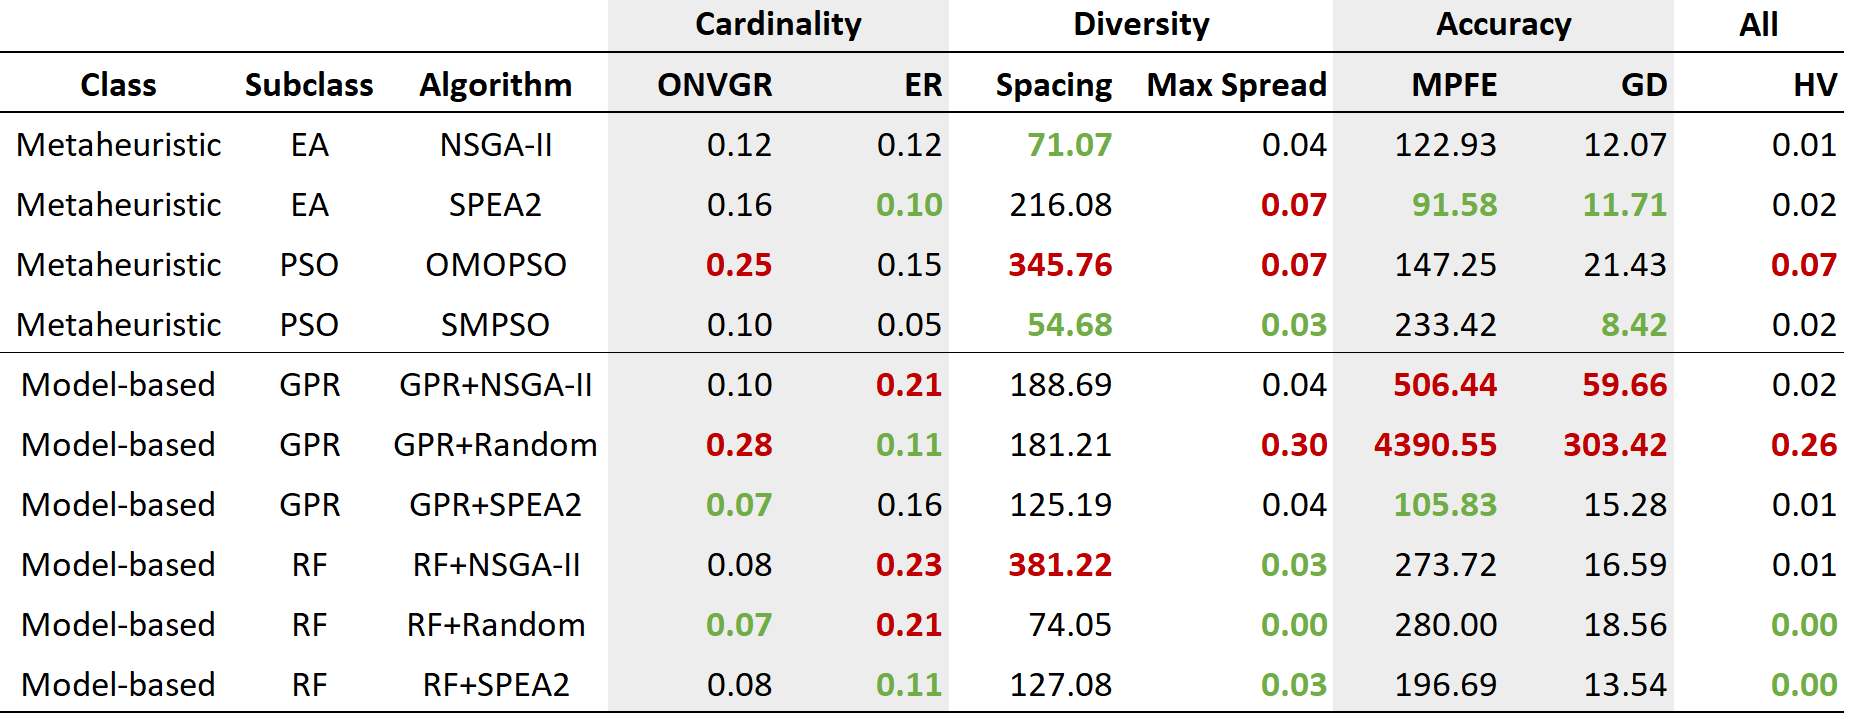
\includegraphics[width=\textwidth]{Images/Evaluation/BlackPavilion/Results_Std_20190428.PNG}
	\caption[Black Pavilion: Standard deviation values for the performance indicators results, discriminated by algorithm]{Black Pavilion: Standard deviation values for the performance indicators results, discriminated by algorithm. Results are averaged over $3$ runs, each with $200$ evaluations.}
	\label{table:blackpavilionstd}
\end{table}

In addition to \ac{MPFE}, we measured the \ac{GD} of each Pareto front. Although the results for this metric resemble the ones obtained with \ac{MPFE}, there are a few differences, namely, in terms of the best performing algorithm. In this case, $RF$+$Random$ is the best algorithm, followed closely by another model-based algorithm, the $GPR$+$SPEA2$. The third and fourth best results correspond to two metaheuristic algorithms, namely, $NSGA$-$II$ and $OMOPSO$, respectively. Other model-based algorithms, like $RF$+$NSGA$-$II$ and $RF$+$SPEA2$ exhibit the fifth and sixth best performance. The two worse algorithms are $GPR$+$NSGA$-$II$ and $GPR$+$Random$. Note, however, that $GPR$+$Random$'s high variance is, once again, mainly due to its poorer performance on the second run. Conversely, the results obtained by $GPR$+$NSGA$-$II$ are relatively distant in the first and third runs (see \cref{sec:blackpavilionextra}).

Finally, we used \ac{HV} to circumvent some of the limitations inherent to other performance indicators, namely, the fact that other indicators exclusively rely on a unique aspect. Contrastingly, \ac{HV} provides a measure of all three aspects. Regarding the \ac{HV}, three algorithms achieved the best result, including a metaheuristic, $NSGA$-$II$, and two model-based algorithms, $RF$+$NSGA$-$II$ and $RF$+$Random$. By observing the \ac{HV} column in \cref{table:blackpavilion}, it is possible to observe that all algorithms with the exception of $OMOPSO$ and $GPR$+$Random$ achieved similar results of \ac{HV}. Once more, the poor performance of $GPR$+$Random$ and $OMOPSO$ during the second run severely hindered their average performance.

%The analysis of the \ac{IGD} indicator revealed that the $RF$+$Random$ was the best algorithm. Surprisingly, the second, third, and fourth best algorithms belong to the metaheuristic class, namely, $SMPSO$, $NSGA$-$II$, and $SPEA2$. These results can be explained by the overall spread of the associated Pareto fronts over the objective space covered by the combined Pareto front, as well as with a more uniform distribution across the objective space. In other words, while $SPEA2$ yields a reasonable number of optimal solutions, each covering regions close to the Pareto solutions' clusters in the combined Pareto front, $GPR$+$SPEA2$ yields a lower number of optimal solutions that fail to cover the different optimal regions identified in the combined Pareto front. Therefore, its \ac{IGD} value will be inherently lower, as \ac{IGD} measures how close the combined Pareto front is to the Pareto fronts identified by each algorithm. When considering the worst algorithms, $GPR$+$NSGA$-$II$ presented the worst performance, followed by $GPR$+$Random$. Their lower performance resulted from the poor distribution of optimal solutions in the objective space, as well as from their generalized inability to discover solutions belonging to the combined Pareto front. 

\begin{figure}[htbp]
	\centering
	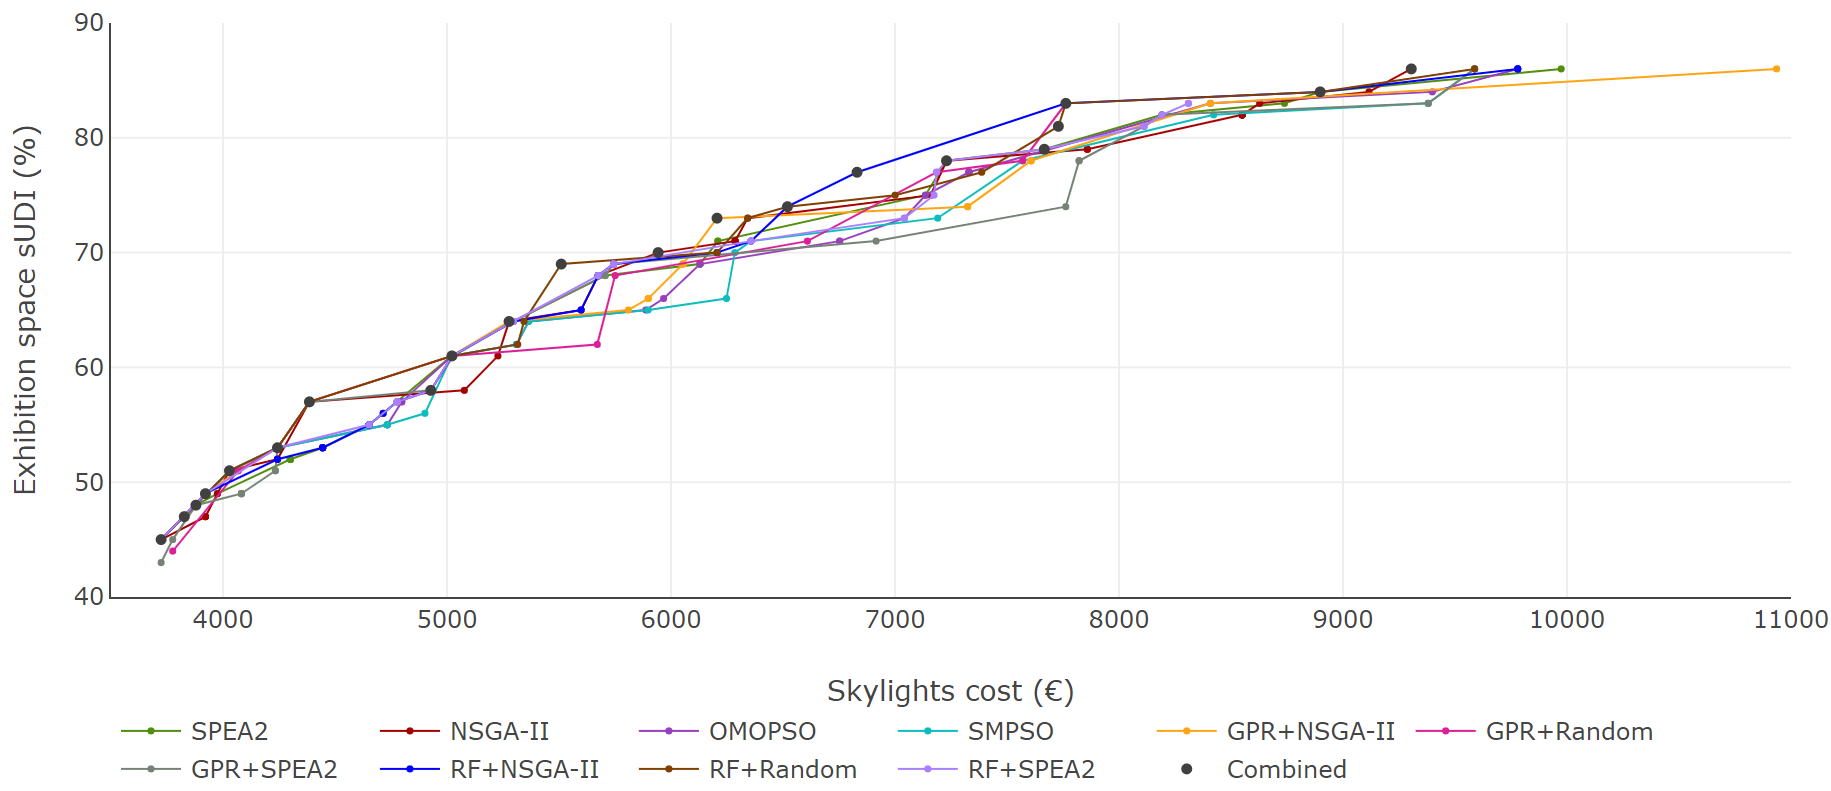
\includegraphics[width=\textwidth]{Images/Evaluation/BlackPavilion/All_Algorithms_all_runs-2019-04-16.png}
	\caption[Black Pavilion: Pareto front plot]{Black Pavilion: Line plot of the Pareto fronts retrieved by each algorithm measuring the daylight conditions of the exhibition space in function of the skylights cost. These fronts are obtained by combining the values of the $3$ runs for each algorithm. The combined Pareto front is formed by finding the nondominated solutions from all the evaluated solutions.}
	\label{fig:blackpavilionallruns}
\end{figure}

\Cref{fig:blackpavilionallruns} presents the overall performance of all the tested algorithms after combining the results of the $3$ runs. We can observe that in general, all algorithms converged towards the combined Pareto front, represented by the black points. Moreover, it is possible to observe that, overall, $RF+Random$, $RF+NSGA$-$II$, and $NSGA$-$II$ converged towards the combined Pareto front with only a few solutions missing the combined Pareto front. On the other hand, algorithms, like $SPEA2$, $SMPSO$, and $GPR+Random$ partially converged to the combined Pareto front, however, for values of cost above $5500$€ these algorithms begin to deviate from the combined Pareto front.

\subsection{Final Remarks}

In this chapter, we have studied the application of different optimization algorithms to three \ac{BPO} case studies. To that end, we have applied the optimization methodology described in \cref{chap:implement}, which uses the Khepri \ac{AD} tool and the optimization framework discussed in \cref{chap:architecture}. We have also used the analytical tools Radiance and Robot to measure the daylight and structural aspects of the different designs generated during the optimization.

The first case study belongs to an unconstrained \ac{SOO} problem, which involved the optimization of the daylight performance of a private house. We tackled this problem in two different ways. On the first stage, we followed a simple design of experiments approach, where we applied two sampling algorithms. On the second stage, we followed an \ac{SOO} approach, for which we have tested $13$ \acp{SOO} derivative-free algorithms, including $5$ direct-search, $5$ model-based, and $3$ metaheuristics. Results showed that, on average, global model-based algorithms exhibit best performance both in earlier and final stages of the optimization process. The same does not happen with metaheuristics that, although exhibiting a reasonable performance in earlier stages of the design, even surpassing the performance of global direct-search algorithms, stagnate shortly after. Conversely, global direct-search algorithms performed reasonably well, excelling metaheuristics shortly after $20$ evaluations. Moreover, we proved that both local direct-search and model-based algorithms can be fast solvers, when provided with reasonable initial solutions. Indeed, two local algorithms converged towards optimal solutions after just $8$ evaluations. Given that each function evaluation took approximately $7$ minutes to complete, this evaluation difference becomes crucial for more complex optimization processes.

The second case study comprises an unconstrained bi-objective optimization problem of an arc-shaped space frame, whose objectives were the structural and the aesthetic aspects of the space frame. To that end, we evaluated the performance of $19$ \acp{MOOA}, $10$ metaheuristics, and $9$ model-based. Given the higher dimensionality of the algorithms' results, we measured the algorithms' performance in terms of the cardinality, diversity, and convergence of the retrieved results. The difficulties underlying \acp{MOOA} quality measurements prevailed during this case study. To circumvent this limitation, we evaluated the algorithms performance through a combination of \ac{MOO} indicators (see \cref{ssec:performance}) and line plots of the Pareto fronts returned by each algorithm. The results showed that \ac{PSO}-based metaheuristics algorithms achieved the overall best performance, whereas \ac{ES}-based metaheuristics algorithms achieved the overall worst performance. Moreover, while model-based algorithms did not outperform any of the metaheuristics algorithms, results suggest that model-based algorithms exploiting \ac{PSO} search strategy outperform other model-based variants, involving $NSGA$-$II$ or $Random$ strategies. Additionally, model-based algorithms depending on $Random$ search strategies seem to perform worse than other variants. 

The third and final case study also comprised an unconstrained bi-objective optimization of the cost and daylight aspects of an art exhibition space. To that end, we tested $10$ \acp{MOOA}, $4$ metaheuristics and $6$ model-based. Similarly to the previous case study, we also used a combination of Pareto front line plots with a set of \ac{MOOA} performance indicators to measure the quality of the optimization results. Results show that, contrastingly to the previous problem, \ac{PSO}-based algorithms fell short in terms of performance. Instead, $RF+Random$, a model-based algorithm, was one of the top performing algorithms, followed by $NSGA$-$II$, a metaheuristic algorithm. 

In conclusion, a thorough analysis of the case studies evidences that there is no single class, subclass, or algorithm that outperforms all others. This corroborates the ideas of Wolpert's optimization \ac{NFLT} \cite{Wolpert1997NFLT}. In the first problem, although global model-based algorithms achieve better results when no information is known, direct-search local algorithms are also able to achieve close to optimal results in fewer iterations. Moreover, while we did not test direct-search algorithms in a \ac{MOO} context problem, it is possible to visualize that even between each category of derivative-free algorithms, either metaheuristic or model-based, different subclasses present significantly different outcomes according to each problem's characteristics. For this reason, we conclude that prior to the selection of an optimization algorithm, users should test different algorithms for a fixed number of evaluations or a fixed amount of time. The proper algorithm selection can have beneficial impacts on the performance of an optimization process, namely in the time and quality of obtained results. In fact, not only do users select the most promising algorithm, but they can also explore the already evaluated solutions to hot-start local algorithms or to create an initial surrogate model. This surrogate model can be explored to determine an approximated behavior of the objective function or to perform optimization. 

Another interesting conclusion is related to the impact of model-based algorithms in \ac{MOO} problems. Although model-based algorithms were not particularly successful in the second case study, they attained relatively better performance in the third case. More comparative \ac{MOO} studies are necessary, especially in \ac{BPO} problems, where studies combining model-based algorithms with Pareto-based optimization approaches are rare. In this vein, this dissertation contributes to bridge this gap and, in the next chapter, we outline future paths of research to further enrich these studies.

Finally, we conclude that there is no consensus regarding the best way to assess the quality of these algorithms and that this comparison should involve the computation of different \ac{MOO} indicators, the visualization of the Pareto front plots, and some critical thinking. 
% If Printing on DOUBLE SIDED pages, the second page should be white.
% Otherwise, comment the following command:
\cleardoublepage
%
%Chapter 6
% #############################################################################
% This is Chapter 6
% !TEX root = ../main.tex
% #############################################################################
% Change the Name of the Chapter i the following line
\fancychapter{Conclusion}
%\cleardoublepage
% The following line allows to ref this chapter
\label{chap:conclusion}

In this chapter, we reflect on the developed work and the obtained results. We draw some general conclusions about the applicability of the solution, including its potential for the architectural practice. We end by outlining some guidelines for future work. 

% #############################################################################
\section{Conclusions}
Nowadays, with the threat of climate change, resource depletion, and worldwide urbanization, it is not enough to construct well-designed buildings, it is also necessary to optimize them \cite{Wortmann2015AdvSBO}. Architectural practices have, therefore, grown to incorporate considerations about the building's performance in various aspects, including energy consumption, comfort, and costs, among others. For the past few decades, the development of computational simulation tools empowered designers with the ability to simulate and estimate a building’s performance, prior to its construction. The emergence of these tools and the raising concerns about the environmental and economic impact of buildings led to the development of new design approaches, such as Performance-Based Design (\ac{PBD}), which seek more efficient design solutions by considering the designs’ performance. Taking design’s performance a step further, optimization has unveilled a new performance-based approach called Building Performance Optimization (\ac{BPO}). 

Unfortunately, traditional \ac{BPO} methodologies require the evaluation of different design variations, which, in turn, implies spending a large amount of time with the manual application of changes to the design and often leading to difficulties when manually modeling complex geometry. Moreover, in order to evaluate a design's performance, the corresponding analytical models must be produced, which also comprises a time-consuming and tiresome task. The emergence of algorithmic-based paradigms, like Algorithmic Design (\ac{AD}) and Algorithmic Analysis (\ac{AA}), enabled the implementation of automated optimization processes, as they allow architects to generate multiple design variants with little effort, to automatically produce the corresponding analytical models, and to automatically evaluate their performance. Notwithstanding the benefits attained with algorithmic approaches, the exploration of more efficient designs still comprises a tiresome and time-consuming task. To overcome this limitation, one can exploit optimization algorithms to more efficiently seek for optimal (or near optimal) design solutions.

Notwithstanding the automation of optimization processes, most \ac{BPO} problems require expensive simulation-based objective functions, for which a single evaluation may take a considerable amount of time to complete. In order to speed up the optimization process, it becomes necessary to identify different optimization algorithms capable of handling the computationally complex problems that characterize \ac{BPO}, and to devise strategies for its efficient application in architecture. Often disregarded, the selection of the appropriate optimization algorithm might have a significant impact in the overall efficiency of optimization processes, and also on the quality of the results \cite{Wolpert1997NFLT}. 

Despite the benefits associated with a more targeted selection of optimization algorithms, most \ac{BPO} practitioners tend to adopt evolutionary-based algorithms \cite{Evins2013, Nguyen2014}. Such algorithms typically require several hundreds or thousands of evaluations, which is an infeasible scenario for most \ac{BPO} problems. Conversely, direct-search methods and model-based algorithms are more promising, typically yielding better results in fewer evaluations \cite{Waibel2018}. One of the main advantages of model-based algorithms is their potential for reducing the overall optimization time \cite{Wortmann2017GABESTCHOICE}, as it was visible in \cref{ssec:soocasestudy}, where the application of global model-based algorithms reduced the overall optimization time, on average, by about $50\%$. 

% What we did, how we tested, what were the conclusions
Along these lines, we studied different optimization approaches and algorithms to measure their affinity for problems involving expensive objective functions, where the number of function evaluations is frequently restricted to a few hundreds \cite{Caetano2018,Belem2018optimizeddesign,Belem2019MOO,IP2019MOO}. We introduced an extension to the \ac{AD} and \ac{AA} approaches, called Algorithmic Optimization (\ac{AO}), which combines an optimization framework with an \ac{AD} tool to allow users to address various design optimization problems, including \ac{BPO}. In general, we conclude that no single class, subclass, or algorithm excels at every problem, thus corroborating the No Free Lunch Theorems (\acp{NFLT}) for optimization \cite{Wolpert1997NFLT}.  

Most tools and, in particular, \ac{MOO} tools, still rely on evolutionary-based algorithms. However, in the evaluated case studies, metaheuristics, especially the evolutionary ones, rarely achieved the best performance. In fact, other categories, such as global model-based or global direct-search algorithms yielded better results. Different factors could change the obtained results (e.g., a different configuration for the algorithms or a lucky random step). Therefore, and contrarily to current architectural practices, we conclude that distinct algorithms behave differently according to the problems' characteristics and that users should test various algorithms for a small number of evaluations or for a short amount of time. 

Furthermore, we conclude that while global optimization algorithms are quicker to converge towards optimal solutions when no additional information is known, local algorithms can be quicker if provided with good starting points and, therefore, should be considered as potential candidates when such information is available.

Regarding the evaluation of different \acp{MOOA}, the lack of consensus regarding the more appropriate way to measure their quality makes it difficult to quantify the suitability of each algorithm for \ac{MOO} problems. In this study, we conclude that algorithms' quality should be measured through the combination of Pareto front plots and multiple performance indicators, namely the cardinality, diversity, and accuracy of the Pareto fronts. %In this way, the real impact of model-based algorithms in the overall optimization time is not quantifiable. To circumvent this limitation, one can measure these indicators per evaluation, similarly to what is done in \ac{SOO} contexts. However, this increases the complexity of the evaluation and requires more standardized ways to measure these algorithms' performance.
 
% Overall conclusion
Based on the conclusions regarding algorithmic efficiency, we believe architects should use several optimization algorithms in their workflow and use the optimization approach that better fits their needs and expertise. This conclusion contradicts the approach taken in some architectural optimization plug-ins, which are often limited to a unique optimization approach and to a small subset of algorithms, namely, the \acp{EA}. Unfortunately, as demonstrated, \acp{EA} are not the best choice for \ac{BPO}. To bypass this limitation, the optimization framework proposed in this dissertation includes different categories of optimization algorithms and facilitates their application by abstracting them under a common interface, thus promoting automated optimization processes. To further facilitate the selection of the most appropriate algorithm, it also includes mechanisms to test multiple optimization algorithms effortlessly. The suitability and capabilities of the framework were evaluated in the context of three \ac{BPO} problems, which demonstrated its ability to solve real architectural problems characterized by computationally complex objective functions.

Overall, as discussed in this dissertation, optimization can be very beneficial for architecture. The combination of simulation tools, algorithmic-based approaches, and optimization algorithms enables the automation of optimization processes within architectural practices. Despite its benefits, the incorrect application of these optimization processes can lead to poor results. Moreover, different architectural design problems benefit most from different optimization algorithms, capable of handling them more efficiently. However, most architectural optimization tools focus on the same subset of algorithms, which are rarely the most adequate algorithms for most problems. The framework proposed in \cref{chap:architecture} overcomes these limitations by providing several optimization algorithms with different characteristics, thus fostering better optimization practices. Finally, the optimization methodology proposed in \cref{chap:implement} was shown to benefit the architectural practice, as was demonstrated by the three \ac{BPO} case studies.
	
% #############################################################################
\section{Limitations and Future Work}
This dissertation proposes a general-purpose optimization framework providing different optimization approaches and optimization algorithms particularly tailored for optimization problems including simulation-based objective functions. Although the current framework already proved valuable to address architectural problems, it can be further improved. In this section, we describe the limitations found and we suggest future lines of research.

% System Limitations
%\subsection{Limitations}
Despite providing the base functionality for addressing optimization problems, the current framework presents some limitations regarding the key aspects mentioned in \cref{ssec:AOW}, namely in terms of (1) flexibility/automation of specific optimization approaches, (2) interactivity, (3) visualization capabilities, and (4) intelligibility of results.

Firstly, notwithstanding the framework support for different optimization approaches (e.g., experimental, Pareto-based), users could also benefit from additional ones, like the prioritization of the optimization of different objectives (e.g., in a bi-objective optimization problem, optimize one objective first and only then proceed to optimize the second). 

Secondly, the current framework does not provide the mechanisms to follow a human-in-the-loop approach, where the user is able to interact and influence the optimization process. The ability to influence the course of an optimization approach would be particularly interesting in the architectural field, where architects can use recently acquired knowledge or intuitions to explore more promising regions of the design space or even to speed up the optimization process. A possible research path includes the ability to change or add constraints in real time or to specify different design variants to be explored, and to influence the search to focus in regions near selected design variants. % The idea is that the user selects a few designs and the optimization will focus on regions near the selected design variants

Thirdly, although the current visualization mechanisms provide a fair and general understanding of the results obtained in optimization processes, they present limitations concerning the visualization of Pareto fronts for problems involving more than three objectives. An important research path is how to represent the information regarding different runs of \ac{MOO} algorithms, for which users have a limited evaluation budget and cannot afford to let the algorithms run indefinitely until they converge towards an ideal Pareto front. %\todo{Referenciar trabalho do Edward Tufte?} 

% Interesting future work
The fourth framework limitation concerns the intelligibility of the produced results. Currently available optimization tools rarely provide information regarding the optimization results, which hinders users' ability to understand them. Besides visual mechanisms and textual logs, our framework does not currently provide additional feedback to aid the user with the interpretation of the optimization results. Therefore, an interesting research path is to explore mechanisms that provide an explanation regarding the quality of the obtained results, especially when using opaque algorithms, i.e., whose non-linearity severely hinders the inteligibility of the optimization process itself. Recent advances in the field of \ac{ML} related to the algorithms' explainability are promising and can be explored to provide explanations about the different optimization algorithms. A starting point to investigate will be to exploit the log files currently produced by the framework and use one of the available model-based methods to approximate the problem and extract information about it using, for example, Layer-wise Relevance Propagation (LRP) or sensitivity analysis techniques \cite{Bach2015,Tripathy2018}.

% Transition
Besides improvements to the framework itself, we also envision other interesting research paths, namely in what concerns the tests and studies of model-based algorithms. 

% \subsection{Future Work}
% Case studies
In fact, although the developed framework was tested in a single-objective daylight optimization case study and two bi-objective optimization case studies, one including the optimization of structural and aesthetics aspects and other incorporating the optimization of daylight and cost aspects, all three case studies involved the optimization of less than six variables with the corresponding bound constraints and at most two objectives. In the future, the proposed framework could be used to test optimization problems with higher complexity, not only in terms of variables and objectives, but also by adding other constraints. Moreover, it would be interesting to assess the performance of optimization algorithms when subject to problems involving other design aspects, including, among others, thermal comfort, energy consumption, and acoustics. 
 
% Optimization algorithms
One other relevant research path is the evaluation of more optimization algorithms, involving different mechanisms and strategies, in order to assess their suitability for optimization problems and its impact on the overall performance of optimization processes. Additionally, as it has been partially demonstrated with the Ericeira's case study, fine-tuning and providing initial information to certain algorithms may drastically improve their performance. For this reason, evaluating the impact of different algorithm's parameters for certain optimization problems would be another relevant case study, particularly, for complex building design problems involving expensive evaluation functions. 

Furthermore, it would be interesting to study the impact of pre-training surrogate-based optimization models based on data obtained from standard optimization test functions~\cite{Zhang2009TEST}. Particularly, users could use previous knowledge about the objectives' behavior (e.g., discontinuous, multimodal, convex) and pre-train the surrogate models in similar standardized test functions, thus, potentially, accelerating optimization processes. In the same vein, testing the impact of approximating the costly evaluation functions using an ensemble of different algorithms could also be exploited to find its impact on the efficiency of the optimization process. %Despite the increased complexity of ensemble techniques, this is can, in general, be neglected in the context of \ac{BPO}, as the overall optimization time tends to be completely dominated by the costly evaluation functions. 
Another interesting study would be to evaluate the impact of using a surrogate model for each objective, instead of using a single one for all objectives. 

% If Printing on DOUBLE SIDED pages, the second page should be white.
% Otherwise, comment the following command:
\cleardoublepage
%
% -----------------------------------------------------------------------------
% BIBLIOGRAPHY
% Add the Bibliography to the PDF table of contents (not the document table of contents)
\pdfbookmark[0]{Bibliography}{bib}
% The bibliography style sheet
% Chose your preferences on the format of the entries and the Labels:
% IEEEtran: Used in general (recommended for IST Thesis)
%           Entries are labelled and sorted by appearance in the document
%           Labels are Numeric inside square brackets
\bibliographystyle{IEEEtran}
%
% Apalike:  Entries formatted alphabetically, last name first, with identation
%           Labels with Autor's Name and Year inside square brackets
%\bibliographystyle{apalike}
%
% Alpha:    Entries formatted with Autor's Name and Year, hanging identation
%           Labels with Autor's abbr. Names and Year inside square brackets
%\bibliographystyle{alpha}
%
% Acm:     Entries formatted with Autor's Name (small Caps), hanging identation
%          Labels are Numeric inside square brackets
%\bibliographystyle{acm}
% The following command resets the 'emphasis' style for bibliography entries
\normalem
% Name of your BiBTeX file
\bibliography{./Thesis-MSc-Bibliography} % Put here your own filename
%
% The following command modifies the 'emphasis' style for bibliography entries
\ULforem
% If Printing on DOUBLE SIDED pages, the second page should be white.
% Otherwise, comment the following command:
\cleardoublepage
%
% -----------------------------------------------------------------------------
% HERE GO THE APPENDIXES IF REQUIRED
% If not required just comment the blocks
\appendix
%% First Appendix
\pdfbookmark[1]{Appendix A}{appendix}
% #############################################################################
% This is Appendix A
% !TEX root = ../main.tex
% #############################################################################
\chapter{Algorithms' Definitions}
\label{appendix:AlgorithmsDefinitions}

A very summarized explanation will be provided for the optimization algorithms studied during this dissertation. Therefore, we suggest \cite{BlumRoli2003Metaheuristics,Glover2003Metaheuristics,Zhou2011} for more complete explanations on metaheuristic algorithms, \cite{Koziel2011} for model-based algorithms, and \cite{Conn2009,Custodio2010,Custodio2018} for direct-search algorithms.

\section{Sampling Algorithms} 
\begin{itemize}
\item \textbf{Full-factorial} generates a complete set of design solutions. Each dimension is described by a discrete set of values, called \textit{levels}. All possible combinations of these levels are generated and used to represent the design space and, thus, minimize errors when running full-factorial techniques multiple times. The number of generated samples scales exponentially with the number of dimensions. 
	
\item \textbf{Monte Carlo Sampling} (or Random Sampling)~\cite{Giunta2003DOE}, originally known as pseudo-Monte Carlo sampling or pseudo-pandom sampling, generates designs randomly. It frequently yields large unexplored regions of the design space. To circunvent this limitation, users should generate several hundreds or thousands of solutions.

\item \textbf{Stratified Monte Carlo Sampling}~\cite{Giunta2003DOE} yields a more uniform sampling of the design space. Each dimension of the design space is subdivided into bins of equal probability and, then, a sample is randomly selected from each bin. Provides better coverage of the design space and allows the user to select the number of bins to create in each dimension. However, the number of generatesd samples scales exponentially with the number of dimensions.

\item \textbf{Latin Hypercube Sampling} (LHS)~\cite{Giunta2003DOE} provides a better distribution of the generated samples by subdividing each dimension in equally sized bins. The generated samples are randomly placed in different bins, so that when observing the one-dimensional projections of the samples and bins, there is only one sample in each bin. The number of samples scales linearly with the number of dimensions.

\end{itemize}

\section{Direct-Search Algorithms}
\begin{itemize}
	\item \textbf{Nelder-Mead Simplex} (NMS)~\cite{Nelder1964} is a local direct-search algorithm that exploits a simplex to enforce convergence towards an optimal solution. The NMS algorithm envelopes a region of the design space using a geometric figure, called simplex, which is a generalization of a triangle or tetrahedron to arbitrary dimensions (e.g., a triangle in two dimensions or a tetrahedron in three dimensions). The simplex is then successively modified using operations, like reflection, expansion, contraction, and shrinking, that iteratively replace the simplex's worst vertex values. Unlike other direct-search algorithms, NMS requires no more than two function evaluations per iteration, except when applying the shrinking operation. The initial simplex has a high impact on the algorithm's performance, particularly, smaller initial simplices frequently lead to local searches and, consequently, to local optimum.
	
	\item \textbf{Subspace simplex} (Subplex)~\cite{Rowan1990} algorithm is an unconstrained local optimization algorithm~\cite{Rowan1990}. As a generalization of the NMS algorithm, SUBPLEX subdivides the design space in low-dimensional subspaces and then applies the NMS algorithm to the most promising subspaces, in order to seek for a better solution. In contrast to NMS, which has difficulties in high-dimensional problems, SUBPLEX reduces the limitations through the decomposition of the problem in low-dimensional subspaces which are more efficiently optimized by NMS.
	
	\item \textbf{Principal Axis} (PRAXIS)~\cite{Brent1973} moves from one region to other by iteratively applying line search algorithms to each direction. The goal of these line search algorithms is to determine a better solution along a certain dimension. It is a local algorithm, which strongly depends on a good initial point.
	
	\item \textbf{DIRECT}~\cite{Jones1993DIRECT} is an algorithm that recursively subdivides the design space into smaller multi-dimensional hyper-rectangles, estimating the quality value of each rectangle. DIRECT uses these values to focus the search on more promising regions of the design space and to further subdivide those in smaller hyper-rectangles. DIRECT is designed to fully explore the variable space, even after finding one or more local optima.
	
	\item \textbf{DIRECT-L} \cite{Gablonsky2001} is a a local variant of DIRECT claimed to be more efficient for functions with few local optima and a single global optimum. The main differences to the original DIRECT algorithm are that DIRECT-L groups the hyper-rectangles based on the size of the longest rectangle side and that there is at most one subdivision in each group, i.e., at most one hyper-rectangle of each group can be subdivided in each iteration. These modifications to the original algorithm promote the reduction of the number of divisions, which has a direct impact on the overall number of function evaluations.
	
	\item \textbf{Direct MultiSearch} DMS \cite{Custodio2010} is a global multi-objective direct-search algorithmic framework which combines the main ideas of directional direct-search algorithms with the Pareto dominance concepts. It maintains a list of feasible nondominated solutions and corresponding step size parameters, which is iteratively updated during the optimization process. From this list, it explores the vicinities of a selected nondominated solution using the associated step size and a predefined set of directions. During the local search around the selected solution, it creates a temporary list of points that contains all the solutions of the first list and the solutions evaluated during this search. The temporary list is then filtered removing any unfeasible or dominated solution. If the temporary list differs from the first list, then it means that better solutions were found and, consequently, the first list is replaced by the temporary one and the process repeats.  On the other hand, if the temporary list equals the first list, it means that the local search was not able to find a better solution and the step size associated to this solution should be reduced. The process then repeats. This algorithmic framework extends to \ac{MOO} the directional direct-search algorithms, including the generalized pattern search and mesh generating set search~\cite{Kolda2003}, among others. 
	 %https://www.mat.uc.pt/~lnv/papers/dms.pdf
	% http://ferrari.dmat.fct.unl.pt/personal/alcustodio/multiglodspaper.pdf


\end{itemize}	

\section{Metaheuristics Algorithms}
\begin{itemize}
	
	\item \textbf{Simulated Annealing} \cite{Brownlee2011} is a global optimization physical algorithm. Resemblant of hill climbing algorithms, where new candidate solutions are randomly sampled, this algorithm iteratively re-samples the solution space aiming at finding an optimal solution. During the search, the algorithm is propitious to accept the re-sampled solutions with lower performance, according to a probabilistic function that becomes more discerning of the quality of the samples over the execution of the algorithm, thus resembling the natural annealing process. 
	
	\item \textbf{Controlled Random Search 2} (CRS2) algorithm is a variant of the CRS algorithm for global optimization~\cite{Price1983}. A CRS algorithm is a population-based random search algorithm that creates an initial set of points, the population, which are then randomly evolved by means of heuristic rules. In the original CRS algorithms, heuristic rules modify a point at a time, replacing the worst point with a better one (called trial point), using a technique resemblant of the NMS algorithm \cite{Nelder1964}. Similarly to NMS, CRS algorithms use a simplex, i.e., a generalized triangle in $N$ dimensions, to envelope a region described by a random subset of points in the population. The worst point of the population is replaced with the reflection of the worst point in the simplex~\cite{Kaelo2006CRS2}. The CRS2 variant differs from the original in that it assumes that the worst population point will always be a part of the simplex. One variant of the CRS2 algorithm introduces a local mutation component in an attempt to overcome situations,  where heuristic rules constantly fail to find a trial points that actually improve the worst point. Fundamentally, this local mutation generates a second trial point that results from the exploitation of the region around the best point in the population~\cite{Kaelo2006CRS2}.  
	
	\item \textbf{Evolutionary Strategy with Cauchy Distribution} (ESCH) \cite{Santos2010} explores evolutionary strategies to seek more efficient solutions. Initially, it creates a population that is iteratively recombined during the optimization according to a non-uniform distribution function and then mutated using a combination of two different mutation operators, such as the Gaussian variation and the gene duplication.
	
	\item \textbf{Improved Stochastic Racking Evolutionary Strategy} (ISRES) \cite{Runarsson2000} is a global evolution strategy method that evolves candidate solutions by stochastically ranking and selecting the best solutions, i.e., a method that maximizes the suitability of the candidate designs given by a fitness ranking function. The candidate designs are evolved iteratively by combining the application of a mutation rule and differential variation.
			
	\item \textbf{Covariance Matrix Adaptation - Evolutionary Strategy} (CMA-ES) \cite{Hansen2006} is a descendent of the evolutionary strategies, whose candidate solutions are sampled according to normal distributions and recombination and mutation amount to selecting new mean values for the distribution and to adding perturbations with zero mean, respectively. CMA-ES maintains a covariance matrix with the pairwise dependencies between the variables in the distribution which is updated using a technique called covariance matrix adaptation (CMA) which attempts to incrementally update the likelihood of previously successful candidate solutions.
	
	\item \textbf{SPEA2} \cite{Zitzler2001SPEA2} is a \ac{MOEA} that incorporates evolutionary mechanisms to incrementally evolve a population from generation to generation. In addition to the population, SPEA2 maintains a set of optimal solutions called archive. While a stopping criteria is not met, the archive is continuously updated by ranking each individual of the population according to the solutions it dominates. Any dominated solution will be removed from the archive and, in case the archive exceeds its size, a clustering technique selects individuals in more crowded regions of the objective space for removal. Binary tournaments are then carried between elements in the archive and population to select the individuals for reproduction and to create the individuals for the next generation, i.e., the offspring. These individuals result from the recombination and mutation of the best individuals from the previous iteration. 
	
	\item \textbf{NSGA-II} \cite{Deb2002} is aa \ac{MOEA} that also incorporates evolutionary mechanisms to incrementally evolve a population. In contrast to SPEA2, NSGA-II does not maintain an archive, instead evaluating a combination of parent and children populations. Initially, a parent population is created and sorted according to its nondomination rank. The nondomination rank is determined as follows: for each individual of the population, determine the nondominated ones and assign those individuals a rank of 1, then, temporarily remove those individuals and, for the remaining individuals, determine the nondominated ones, assigning those individuals a rank of 2, repeating this process repeat until every individual is assigned a rank. After assigning these ranks, NSGA-II applies binary tournaments, based on the nondomination rank, to select the individuals to recombine and mutate in order to create the initial children population. Afterwards, both parent and children populations are combined. For each individual, NSGA-II computes the nondomination rank and a density of estimate based on the average distance of the two closest individuals. The best individuals compose, what the algorithm calls a new parent population, which is then sorted according to their rank and density estimates. Again, the parent population is subject to binary tournaments, which now consider both the nondomination rank and the density measure, to select the individuals for reproduction. These individuals are then recombined and mutated, thus producing the new children population. The process then repeats until a stopping criteria is met, combining the new parent and children populations and recomputing their nondomination rank and diversity measures and generating the new populations for the next iteration.
	
	
	\item \textbf{Epsilon-\ac{MOEA}} ($\epsilon$-MOEA) 
	
	\item \textbf{Hypervolume Estimation Algorithm for \ac{MOO}} (HypE)~\cite{Zitzler2011HypE} an algorithm that explores the \ac{HV} indicator to rank individuals. Particularly, to minimize time penalties associated with the computation of the \ac{HV}, in scenarios with more than three objectives, HypE uses Monte Carlo simulations to estimate the \ac{HV} value of each individual.
% 	Unfortunately, algorithms incorporating the Pareto dominance relation and diversity measures appear to have difficulties in optimization scenarios with more than two objectives, which spurred the development of algorithms using other quality measures, including quality indicators. To overcome the objective limitation and provide the user with the flexibility to use a more efficient algorithm, Octopus provides the option to use HypE, an algorithm that explores the \ac{HV} indicator to rank individuals. Particularly, to minimize time penalties associated with the computation of the \ac{HV}, in scenarios with more than three objectives, HypE uses Monte Carlo simulations to estimate the \ac{HV} value of each individual~\cite{Zitzler2011HypE}. 
	
	\item \textbf{\ac{MOEA} with Decomposition} (MOEA/D)
	
	\item \textbf{Pareto Archived Evolution Strategy} (PAES) is a \ac{MOEA} which explores \acp{ES} on populations composed of a single individual and maintains an archive with previously found solutions to identify the approximate dominance ranking of the current and candidate solution vectors. In every iteration, the candidate solution is compared with respect to the current solution and depending on whether the candidate dominates the current solution or not, the current solution will be updated or a new candidate solution is found through mutation. In the case where none of the solutions dominate each other, each solution is compared against an archive of the nondominated solutions and if the candidate solution dominates any of the solutions in the archive, it will be accepted as the new current solution and the dominated solutions are removed from the archive, otherwise, the selection of the new current solution will be based on how crowded each solution is, when compared to the solutions in the archive. 
		
	\item \textbf{Pareto Envelope-Based Selection Algorithm 2} (PESA2)
	
	\item \textbf{Speed-constrained Multi-objective \ac{PSO}} (SMPSO)
	
	\item \textbf{OMOPSO}
	
\end{itemize}

\section{Model-based Algorithms}
\begin{itemize}
	\item \textbf{GPR-based} algorithms rely on guassian process (GP) techniques, which generalize Gaussian probability distributions to functions. GP algorithms incorporate a measure of the similarity between points, called the kernel function, to predict the value for an unseen point from training data. Besides the prediction of the value, GPs provide a measure of the associated uncertainty.
	
	\item \textbf{MLP-based} algorithms consist on the creation of surrogate models using \acp{MLP}. \ac{MLP} is a class of feedforward neural networks that comprises at least three layers of nodes, including one input layer, one output layer, and, at least, one hidden layer. In neural networks, all nodes with the exception of the input nodes are called neurons and each node possesses a non-linear activation function. These non-linearities provide the networks the ability to approximate non-linear and extremely complex functions. These \acp{MLP} models are trained using a supervised learning technique, where the model is provided with the input variables' values and the outcome that was observed for those input values. The model is then updated using a technique called backpropagation which uses the error rates between the obtained outcome and the expected outcome to correct the neurons and improve the \ac{MLP} model. 
	
	\item \textbf{RBF-based} algorithms consist on the creation of surrogate models using \acp{RBF}. Since its invention, multiple implementations of \ac{RBF} have been proposed. RBFOpt implements two well-known versions, namely, the Gutmann's~\cite{Gutmann2001} and the Regis and Shoemaker's~\cite{Regis2007}, commonly known as MSRSM. These techniques differ in the search strategy for the next candidate solution to be evaluated using the original objective function. The former uses the solution, which is likely to yield the largest improvement in the surrogate's accuracy, whereas the latter tries to balance the surrogate's accuracy amelioration with the exploitation of promising solutions, using other search strategies, such as genetic algorithms, sampling algorithms, or other mathematical solvers~\cite{Wortmann2017Opossum}. Moreover, RBFOpt provides five different types of radial basis function: linear, multi-quadratic, cubic, thin plate spline, and automatic selection, which are also provided in the Opossum interface.
		
	\item \textbf{RF-based} algorithms consist on the creation of surrogate models using \acp{RF}, also called random decision forests~\cite{Ho1995RDF}. These algorithms incorporate an ensemble learning approach that consists on applying multiple decision trees to obtain a better performance. Given a set of input variables the result of an \ac{RF} algorithm will be given by the mean  of the results returned by each individual tree. \ac{RF} are particularly sought due to their ability to correct the decision trees propensity to overfit the data, i.e., to become too specific.
	
\end{itemize}
%% If Printing on DOUBLE SIDED pages, the second page should be white.
%% Otherwise, comment the following command:
\cleardoublepage
%% Second Appendix
\pdfbookmark[1]{Appendix B}{appendix}
% #############################################################################
% This is Appendix B
% !TEX root = ../main.tex
% #############################################################################
\appendix\chapter{Extra Case studies}
\label{appendix:appendixB}

\section{Space Frame Optimization: Algorithms' Runs}
\label{sec:spaceframeoptimizationextra}

\begin{figure}[htbp]
	\centering
	\includegraphics[width=\textwidth]{Images/Evaluation/caadria/All_Algorithms_run1-2019-04-13.png}
	\caption[Space Frame: Pareto Fronts for run 1]{Space Frame: Algorithms' Pareto fronts for the bi-objective space frame optimization problem. Pareto fronts based on the results of run 1. The combined Pareto front is composed of the optimal solutions found during run 1.}
	\label{table:spaceframerun1}
\end{figure}

\begin{figure}[htbp]
	\centering
	\includegraphics[width=\textwidth]{Images/Evaluation/caadria/All_Algorithms_run2-2019-04-13_1.png}
	\caption[Space Frame: Pareto Fronts for run 2]{Space Frame: Algorithms' Pareto fronts for the bi-objective space frame optimization problem. Pareto fronts based on the results of run 2. The combined Pareto front is composed of the optimal solutions found during run 2.}
	\label{table:spaceframesrun2}
\end{figure}

\begin{figure}[htbp]
	\centering
	\includegraphics[width=\textwidth]{Images/Evaluation/caadria/All_Algorithms_run3-2019-04-13.png}
	\caption[Space Frame: Pareto Fronts for run 3]{Space Frame: Algorithms' Pareto fronts for the bi-objective space frame optimization problem. Pareto fronts based on the results of run 3. The combined Pareto front is composed of the optimal solutions found during run 3.}
	\label{table:spaceframerun3}
\end{figure}
%% If Printing on DOUBLE SIDED pages, the second page should be white.
%% Otherwise, comment the following command:
\cleardoublepage

% -----------------------------------------------------------------------------
% And this is THE END of the IST Thesis Document
\end{document}